% ------------------------------------------------------------
% LaTeX Template für die DHBW zum Schnellstart!
% Original: https://github.wdf.sap.corp/vtgermany/LaTeX-Template-DHBW
% ------------------------------------------------------------
% ---- Präambel mit Angaben zum Dokument
\documentclass[
	fontsize=12pt,           % Leitlinien sprechen von Schriftgröße 12.
	paper=A4,
	twoside=false,
	listof=totoc,            % Tabellen- und Abbildungsverzeichnis ins Inhaltsverzeichnis
	bibliography=totoc,      % Literaturverzeichnis ins Inhaltsverzeichnis aufnehmen
	titlepage,               % Titlepage-Umgebung anstatt \maketitle
	headsepline,             % horizontale Linie unter Kolumnentitel
	abstract,              % Überschrift einschalten, Abstract muss in {abstract}-Umgebung stehen
]{scrreprt}                  % Verwendung von KOMA-Report
\usepackage[utf8]{inputenc}  % UTF8 Encoding einschalten
\usepackage[ngerman]{babel}  % Neue deutsche Rechtschreibung
\usepackage[T1]{fontenc}     % Ausgabe von westeuropäischen Zeichen (auch Umlaute)
\usepackage{microtype}       % Trennung von Wörtern wird besser umgesetzt
\usepackage{lmodern}         % Nicht-gerasterte Schriftarten (bei MikTeX erforderlich)
\usepackage{graphicx}        % Einbinden von Grafiken erlauben
\usepackage{wrapfig}         % Grafiken fließend im Text
\usepackage{setspace}        % Zeilenabstand \singlespacing, \onehalfspaceing, \doublespacing
\usepackage[
	%showframe,                % Ränder anzeigen lassen
	left=2.7cm, right=2.5cm,
	top=2.5cm,  bottom=2.5cm,
	includeheadfoot
]{geometry}                      % Seitenlayout einstellen
\usepackage{scrlayer-scrpage}    % Gestaltung von Fuß- und Kopfzeilen
\usepackage{acronym}             % Abkürzungen, Abkürzungsverzeichnis
\usepackage{titletoc}            % Anpassungen am Inhaltsverzeichnis
\contentsmargin{0.75cm}          % Abstand im Inhaltsverzeichnis zw. Punkt und Seitenzahl
\usepackage[                     % Klickbare Links (enth. auch "nameref", "url" Package)
  hidelinks,                     % Blende die "URL Boxen" aus.
  breaklinks=true                % Breche zu lange URLs am Zeilenende um
]{hyperref}
\usepackage[hypcap=true]{caption}% Anker Anpassung für Referenzen
\urlstyle{same}                  % Aktuelle Schrift auch für URLs
% Anpassung von autoref für Gleichungen (ergänzt runde Klammern) und Algorithm.
% Anstatt "Listing" kann auch z.B. "Code-Ausschnitt" verwendet werden. Dies sollte
% jedoch synchron gehalten werden mit \lstlistingname (siehe weiter unten).
\addto\extrasngerman{%
	\def\equationautorefname~#1\null{Gleichung~(#1)\null}
	\def\lstnumberautorefname{Zeile}
	\def\lstlistingautorefname{Listing}
	\def\algorithmautorefname{Algorithmus}
	% Damit einheitlich "Abschnitt 1.2[.3]" verwendet wird und nicht "Unterabschnitt 1.2.3"
	% \def\subsectionautorefname{Abschnitt}
}

% ---- Abstand verkleinern von der Überschrift 
\renewcommand*{\chapterheadstartvskip}{\vspace*{.5\baselineskip}}

% Hierdurch werden Schusterjungen und Hurenkinder vermieden, d.h. einzelne Wörter
% auf der nächsten Seite oder in einer einzigen Zeile.
% LaTeX kann diese dennoch erzeugen, falls das Layout ansonsten nicht umsetzbar ist.
% Diese Werte sind aber gute Startwerte.
\widowpenalty10000
\clubpenalty10000

% ---- Für das Quellenverzeichnis
\usepackage[
	backend = biber,                % Verweis auf biber
	language = auto,
	style = numeric,                % Nummerierung der Quellen mit Zahlen
	sorting = none,                 % none = Sortierung nach der Erscheinung im Dokument
	sortcites = true,               % Sortiert die Quellen innerhalb eines cite-Befehls
	block = space,                  % Extra Leerzeichen zwischen Blocks
	hyperref = true,                % Links sind klickbar auch in der Quelle
	%backref = true,                % Referenz, auf den Text an die zitierte Stelle
	bibencoding = auto,
	giveninits = true,              % Vornamen werden abgekürzt
	doi=false,                      % DOI nicht anzeigen
	isbn=false,                     % ISBN nicht anzeigen
    alldates=short                  % Datum immer als DD.MM.YYYY anzeigen
]{biblatex}
\addbibresource{Inhalt/literatur.bib}
\setcounter{biburlnumpenalty}{3000}     % Umbruchgrenze für Zahlen
\setcounter{biburlucpenalty}{6000}      % Umbruchgrenze für Großbuchstaben
\setcounter{biburllcpenalty}{9000}      % Umbruchgrenze für Kleinbuchstaben
\DeclareNameAlias{default}{family-given}  % Nachname vor dem Vornamen
\AtBeginBibliography{\renewcommand{\multinamedelim}{\addslash\space
}\renewcommand{\finalnamedelim}{\multinamedelim}}  % Schrägstrich zwischen den Autorennamen
\DefineBibliographyStrings{german}{
  urlseen = {Einsichtnahme:},                      % Ändern des Titels von "besucht am"
}
\usepackage[babel,german=quotes]{csquotes}         % Deutsche Anführungszeichen + Zitate


% ---- Für Mathevorlage
\usepackage{amsmath}    % Erweiterung vom Mathe-Satz
\usepackage{amssymb}    % Lädt amsfonts und weitere Symbole
\usepackage{MnSymbol}   % Für Symbole, die in amssymb nicht enthalten sind.


% ---- Für Quellcodevorlage
\usepackage{scrhack}                    % Hack zur Verw. von listings in KOMA-Script
\usepackage{listings}                   % Darstellung von Quellcode
\usepackage{xcolor}                     % Einfache Verwendung von Farben
% -- Eigene Farben für den Quellcode
\definecolor{JavaLila}{rgb}{0.4,0.1,0.4}
\definecolor{JavaGruen}{rgb}{0.3,0.5,0.4}
\definecolor{JavaBlau}{rgb}{0.0,0.0,1.0}
\definecolor{ABAPKeywordsBlue}{HTML}{6000ff}
\definecolor{ABAPCommentGrey}{HTML}{808080}
\definecolor{ABAPStringGreen}{HTML}{4da619}
\definecolor{PyKeywordsBlue}{HTML}{0000AC}
\definecolor{PyCommentGrey}{HTML}{808080}
\definecolor{PyStringGreen}{HTML}{008080}
% -- Farben für ABAP CDS
\definecolor{CDSString}{HTML}{FF8C00}
\definecolor{CDSKeywords}{HTML}{6000ff}
\definecolor{CDSAnnotation}{HTML}{00BFFF}
\definecolor{CDSComment}{HTML}{808080}
\definecolor{CDSFunc}{HTML}{FF0000}

% -- Default Listing-Styles

\lstset{
	% Das Paket "listings" kann kein UTF-8. Deswegen werden hier 
	% die häufigsten Zeichen definiert (ä,ö,ü,...)
	literate=%
		{á}{{\'a}}1 {é}{{\'e}}1 {í}{{\'i}}1 {ó}{{\'o}}1 {ú}{{\'u}}1
		{Á}{{\'A}}1 {É}{{\'E}}1 {Í}{{\'I}}1 {Ó}{{\'O}}1 {Ú}{{\'U}}1
		{à}{{\`a}}1 {è}{{\`e}}1 {ì}{{\`i}}1 {ò}{{\`o}}1 {ù}{{\`u}}1
		{À}{{\`A}}1 {È}{{\'E}}1 {Ì}{{\`I}}1 {Ò}{{\`O}}1 {Ù}{{\`U}}1
		{ä}{{\"a}}1 {ë}{{\"e}}1 {ï}{{\"i}}1 {ö}{{\"o}}1 {ü}{{\"u}}1
		{Ä}{{\"A}}1 {Ë}{{\"E}}1 {Ï}{{\"I}}1 {Ö}{{\"O}}1 {Ü}{{\"U}}1
		{â}{{\^a}}1 {ê}{{\^e}}1 {î}{{\^i}}1 {ô}{{\^o}}1 {û}{{\^u}}1
		{Â}{{\^A}}1 {Ê}{{\^E}}1 {Î}{{\^I}}1 {Ô}{{\^O}}1 {Û}{{\^U}}1
		{œ}{{\oe}}1 {Œ}{{\OE}}1 {æ}{{\ae}}1 {Æ}{{\AE}}1 {ß}{{\ss}}1
		{ű}{{\H{u}}}1 {Ű}{{\H{U}}}1 {ő}{{\H{o}}}1 {Ő}{{\H{O}}}1
		{ç}{{\c c}}1 {Ç}{{\c C}}1 {ø}{{\o}}1 {å}{{\r a}}1 {Å}{{\r A}}1
		{€}{{\euro}}1 {£}{{\pounds}}1 {«}{{\guillemotleft}}1
		{»}{{\guillemotright}}1 {ñ}{{\~n}}1 {Ñ}{{\~N}}1 {¿}{{?`}}1,
	breaklines=true,        % Breche lange Zeilen um 
	breakatwhitespace=true, % Wenn möglich, bei Leerzeichen umbrechen
	% Symbol für Zeilenumbruch einfügen
	prebreak=\raisebox{0ex}[0ex][0ex]{\ensuremath{\rhookswarrow}},
	postbreak=\raisebox{0ex}[0ex][0ex]{\ensuremath{\rcurvearrowse\space}},
	tabsize=4,                                 % Setze die Breite eines Tabs
	basicstyle=\ttfamily\small,                % Grundsätzlicher Schriftstyle
	columns=fixed,                             % Besseres Schriftbild
	numbers=left,                              % Nummerierung der Zeilen
	%frame=single,                             % Umrandung des Codes
	showstringspaces=false,                    % Keine Leerzeichen hervorheben
	keywordstyle=\color{blue},
	ndkeywordstyle=\bfseries\color{darkgray},
	identifierstyle=\color{black},
	commentstyle=\itshape\color{JavaGruen},   % Kommentare in eigener Farbe
	stringstyle=\color{JavaBlau},             % Strings in eigener Farbe,
	captionpos=b,                             % Bild*unter*schrift
	xleftmargin=5.0ex
}

% ---- Eigener JAVA-Style für den Quellcode
\renewcommand{\ttdefault}{pcr}               % Schriftart, welche auch fett beinhaltet
\lstdefinestyle{EigenerJavaStyle}{
	language=Java,                             % Syntax Highlighting für Java
	%frame=single,                             % Umrandung des Codes
	keywordstyle=\bfseries\color{JavaLila},    % Keywords in eigener Farbe und fett
	commentstyle=\itshape\color{JavaGruen},    % Kommentare in eigener Farbe und italic
	stringstyle=\color{JavaBlau}               % Strings in eigener Farbe
}

% ---- Eigener ABAP-Style für den Quellcode
\renewcommand{\ttdefault}{pcr}
\lstdefinestyle{EigenerABAPStyle}{
	language=[R/3 6.10]ABAP,
	morestring=[b]\|,                          % Für Pipe-Strings
	morestring=[b]\`,                          % für Backtick-Strings
	keywordstyle=\bfseries\color{ABAPKeywordsBlue},
	commentstyle=\itshape\color{ABAPCommentGrey},
	stringstyle=\color{ABAPStringGreen},
	tabsize=2,
	morekeywords={
		types,
		@data,
		as,
		lower,
		start,
		selection,
		order,
		by,
		inner,
		join,
		key,
		end,
		cast
	}
}

% ---- Eigener Python-Style für den Quellcode
\renewcommand{\ttdefault}{pcr}
\lstdefinestyle{EigenerPythonStyle}{
	language=Python,
	columns=flexible,
	keywordstyle=\bfseries\color{PyKeywordsBlue},
	commentstyle=\itshape\color{PyCommentGrey},
	stringstyle=\color{PyStringGreen}
}

%----- ABAP-CDS-View language
\lstdefinelanguage{ABAPCDS}{
	sensitive=false,
	%Keywords
	morekeywords={define,
		view,
		as,
		select,
		from,
		inner,
		join,
		on,
		key,
		case,
		when,
		then,
		else,
		end,
		true,
		false,
		cast,
		where,
		and,
		distinct,
		group,
		by,
		having,
		min,
		sum,
		max,
		count,
		avg
	},
	%Methoden
	morekeywords=[2]{
		div,
		currency\_conversion,
		dats\_days\_between,
		concat\_with\_space,
		dats\_add_days,
		dats\_is\_valid,
		dats\_add\_months,
		unit\_conversion,
		division,
		mod,
		abs,
		floor,
		ceil,
		round,
		concat,
		replace,
		substring,
		left,
		right,
		length
	},
	morecomment=[s][\color{CDSAnnotation}]{@}{:},
	morecomment=[l][\itshape\color{CDSComment}]{//},
	morecomment=[s][\itshape\color{CDSComment}]{/*}{*/},
	morestring=[b][\color{CDSString}]',
	keywordstyle=\bfseries\color{CDSKeywords},
	keywordstyle=[2]\color{CDSFunc}
}

  % Weitere Details sind ausgelagert

\usepackage{algorithm}                  % Für Algorithmen-Umgebung (ähnlich wie lstlistings Umgebung)
\usepackage{algpseudocode}              % Für Pseudocode. Füge "[noend]" hinzu, wenn du kein "endif",
                                        % etc. haben willst.

\makeatletter                           % Sorgt dafür, dass man @ in Namen verwenden kann.
                                        % Ansonsten gibt es in der nächsten Zeile einen Compilefehler.
\renewcommand{\ALG@name}{Algorithmus}   % Umbenennen von "Algorithm" im Header der Listings.
\makeatother                            % Zeichen wieder zurücksetzen
\renewcommand{\lstlistingname}{Listing} % Erlaubt das Umbenennen von "Listing" in anderen Titel.

% ---- Tabellen
\usepackage{booktabs}  % Für schönere Tabellen. Enthält neue Befehle wie \midrule
\usepackage{multirow}  % Mehrzeilige Tabellen
\usepackage{siunitx}   % Für SI Einheiten und das Ausrichten Nachkommastellen
\sisetup{locale=DE, range-phrase={~bis~}, output-decimal-marker={,}} % Damit ein Komma und kein Punkt verwendet wird.
\usepackage{xfrac} % Für siunitx Option "fraction-function=\sfrac"

% ---- Für Definitionsboxen in der Einleitung
\usepackage{amsthm}                     % Liefert die Grundlagen für Theoreme
\usepackage[framemethod=tikz]{mdframed} % Boxen für die Umrandung
% ---- Definition für Highlight Boxen

% ---- Grundsätzliche Definition zum Style
\newtheoremstyle{defi}
  {\topsep}         % Abstand oben
  {\topsep}         % Abstand unten
  {\normalfont}     % Schrift des Bodys
  {0pt}             % Einschub der ersten Zeile
  {\bfseries}       % Darstellung von der Schrift in der Überschrift
  {:}               % Trennzeichen zwischen Überschrift und Body
  {.5em}            % Abstand nach dem Trennzeichen zum Body Text
  {\thmname{#3}}    % Name in eckigen Klammern
\theoremstyle{defi}

% ------ Definition zum Strich vor eines Texts
\newmdtheoremenv[
  hidealllines = true,       % Rahmen komplett ausblenden
  leftline = true,           % Linie links einschalten
  innertopmargin = 0pt,      % Abstand oben
  innerbottommargin = 4pt,   % Abstand unten
  innerrightmargin = 0pt,    % Abstand rechts
  linewidth = 3pt,           % Linienbreite
  linecolor = gray!40,       % Linienfarbe
]{defStrich}{Definition}     % Name der des formats "defStrich"

% ------ Definition zum Eck-Kasten um einen Text
\newmdtheoremenv[
  hidealllines = true,
  innertopmargin = 6pt,
  linecolor = gray!40,
  singleextra={              % Eck-Markierungen für die Definition
    \draw[line width=3pt,gray!50,line cap=rect] (O|-P) -- +(1cm,0pt);
    \draw[line width=3pt,gray!50,line cap=rect] (O|-P) -- +(0pt,-1cm);
    \draw[line width=3pt,gray!50,line cap=rect] (O-|P) -- +(-1cm,0pt);
    \draw[line width=3pt,gray!50,line cap=rect] (O-|P) -- +(0pt,1cm);
  }
]{defEckKasten}{Definition}  % Name der des formats "defEckKasten"  % Weitere Details sind ausgelagert

% ---- Für Todo Notes
\usepackage{todonotes}
\setlength {\marginparwidth }{2cm}      % Abstand für Todo Notizen

\usepackage{placeins}


% ---- Elektronische Version oder Gedruckte Version?
% ---- Unterschied: Die elektronische Version enthält keinen Platzhalter für die Unterschrift
\usepackage{ifthen}
\newboolean{e-Abgabe}
\setboolean{e-Abgabe}{false}    % false=gedruckte Fassung

% ---- Persönlichen Daten:
\newcommand{\titel}{Programmentwurf \\ DnD-Character Manager}
\newcommand{\titelheader}{DnD-Character Manager}
%\newcommand{\arbeit}{Projektarbeit 1 (T3\_2000)}
%\newcommand{\studiengang}{Informatik}
%\newcommand{\studienjahr}{2015}
\newcommand{\autor}{Leon Knorr}
\newcommand{\autorReverse}{Knorr, Leon}
\newcommand{\verfassungsort}{Karlsruhe}
\newcommand{\matrikelnr}{9800840}
%\newcommand{\kurs}{TINF15B1}
%\newcommand{\bearbeitungsmonat}{Januar 2018}
\newcommand{\abgabe}{01. Februar 2018}
%\newcommand{\bearbeitungszeitraum}{01.10.2017 - 31.01.2018}
%\newcommand{\firmaName}{SAP SE}
%\newcommand{\firmaStrasse}{Dietmar-Hopp-Allee 16}
%\newcommand{\firmaPlz}{69190 Walldorf, Deutschland}
%\newcommand{\betreuerFirma}{B-Vorname B-Nachname}
%\newcommand{\betreuerDhbw}{DH-Vorname DH-Nachname}

% ---- Metainformation für das PDF Dokument
\hypersetup{
	pdftitle    = {\titel},
	pdfauthor   = {\autor},
	%pdfkeywords = {Keywords angeben},
	pdfcreator  = {LaTeX},
	%pdfproducer = {in der Regel pdfTeX}
}

% ---- Definition der Kopf- und Fußzeilen
\clearpairofpagestyles                          % Löschen von LaTeX Standard
\automark[section]{chapter}                     % Füllen von section und chapter
\renewcommand*{\chaptermarkformat}{}            % Entfernt die Kapitelnummer
\renewcommand*{\sectionmarkformat}{}            % Entfernt die Sectionnummer
% Angaben [für "plain"]{für "scrheadings"}
\ihead[]{\titelheader}                          % Kopfzeile links
\chead[]{}                                      % Kopfzeile mitte
\ohead[]{\rightmark}                            % Kopfzeile rechts
\ifoot[]{}                                      % Fußzeile links
\cfoot*{\sffamily\pagemark}                     % Fußzeile mitte
\ofoot[]{}                                      % Fußzeile rechts
\KOMAoptions{
   headsepline = 0.2pt,                         % Liniendicke Kopfzeile
   footsepline = false                          % Liniendicke Fußzeile
}


% ---- Hilfreiches
\newcommand{\zB}{z.\,B. }   % "z.B." mit kleinem Leeraum dazwischen (ohne wäre nicht korrekt)
\newcommand{\dash}{d.\,h. }

\newcommand{\code}[1]{\texttt{#1}} % Ist einfacher zu schreiben als ständig \texttt und erlaubt
                                   % Änderungen im Nachhinein, wenn man z.B. Inline-Code anders stylen möchte.

% ---- Silbentrennung (falls LaTeX defaults falsch / nicht gewünscht sind)
\hyphenation{HANA}         % anstatt HA-NA
\hyphenation{Graph-Script} % anstatt GraphS-cript

% ---- Beginn des Dokuments
\begin{document}
\setlength{\parindent}{0pt}              % Keine Paragraphen Einrückung.
                                         % Dafür haben wir den Abstand zwischen den Paragraphen.
\setcounter{secnumdepth}{2}              % Nummerierungstiefe fürs Inhaltsverzeichnis
\setcounter{tocdepth}{1}                 % Tiefe des Inhaltsverzeichnisses. Ggf. so anpassen,
                                         % dass das Verzeichnis auf eine Seite passt.
\sffamily                                % Serifenlose Schrift verwenden.

% ---- Vorspann
% ------ Titelseite
\singlespacing
\thispagestyle{empty}
\begin{titlepage}
\enlargethispage{4cm}

%\begin{figure}           % Logo vom Ausbildungsbetrieb und der DHBW
	% \vspace*{-5mm} % Sollte dein Titel zu lang werden, kannst du mit diesem "Hack" 
	%                  den Inhalt der Seite nach oben schieben.
%	\begin{minipage}{0.49\textwidth}
%		\flushleft
%		
\includegraphics[height=2.5cm]{Bilder/Logos/Logo_SAP.pdf} 
%	\end{minipage}
%	\hfill
%	\begin{minipage}{0.49\textwidth}
%		\flushright
%		
\includegraphics[height=2.5cm]{Bilder/Logos/Logo_DHBW.pdf} 
%	\end{minipage}
%\end{figure} 
%\vspace*{0.1cm}

\huge{\textbf{\titel}}\\[1.5cm]
\begin{tabular}{ll}
    Name:                            & \autor \\[0.2cm]
    Matrikelnummer:                  & \matrikelnr \\[0.2cm]
	Abgabedatum:                     & \abgabe \\[0.2cm]
\end{tabular} 
\end{titlepage}
  % Titelseite
\newcounter{savepage}
\pagenumbering{Roman}                    % Römische Seitenzahlen
\onehalfspacing

% ------ Erklärung, Sperrvermerk, Abstact
%\chapter*{Eidesstattliche Erklärung}
Ich versichere hiermit, dass ich meine \arbeit{} mit dem Thema:
\begin{quote}
	\textit{\titel}
\end{quote} 
gemäß § 5 der \enquote{Studien- und Prüfungsordnung DHBW Technik} vom 29. September 2017 selbstständig verfasst und keine anderen als die angegebenen Quellen und Hilfsmittel benutzt habe. Die Arbeit wurde bisher keiner anderen Prüfungsbehörde vorgelegt und auch nicht veröffentlicht.

\vspace{0.25cm}

Ich versichere zudem, dass die eingereichte elektronische Fassung mit der gedruckten Fassung übereinstimmt.

\vspace{1cm}

\verfassungsort, den \today \\[0.5cm]
\ifthenelse{\boolean{e-Abgabe}}
	{\underline{Gez. \autor}}
	{\makebox[6cm]{\hrulefill}}\\ 
\autorReverse

%\chapter*{Sperrvermerk}
Die nachfolgende Arbeit enthält vertrauliche Daten der:
\begin{quote}
	\firmaName \\
	\firmaStrasse \\
	\firmaPlz
\end{quote}

\vspace{0.5cm}

Der Inhalt dieser Arbeit darf weder als Ganzes noch in Auszügen Personen außerhalb des Prüfungsprozesses und des Evaluationsverfahrens zugänglich gemacht werden, sofern keine anderslautende Genehmigung vom Dualen Partner vorliegt.

%\renewcommand{\abstractname}{Abstract} % Veränderter Name für das Abstract
\begin{abstract}
\begin{addmargin}[1.5cm]{1.5cm}        % Erhöhte Ränder, für Abstract Look
\thispagestyle{plain}                  % Seitenzahl auf der Abstract Seite

\begin{center}
\small\textit{- English -}             % Angabe der Sprache für das Abstract
\end{center}

\vspace{0.25cm}

This is the starting point of the Abstract. For the final bachelor thesis, there must be an abstract included in your document. So, start now writing it in German and English. The abstract is a short summary with around 200 to 250 words.

\vspace{0.25cm}

Try to include in this abstract the main question of your work, the methods you used or the main results of your work.


\end{addmargin}
\end{abstract}
%\renewcommand{\abstractname}{Abstract} % Veränderter Name für das Abstract
\begin{abstract}
\begin{addmargin}[1.5cm]{1.5cm}        % Erhöhte Ränder, für Abstract Look
\thispagestyle{plain}                  % Seitenzahl auf der Abstract Seite

\begin{center}
\small\textit{- Deutsch -}             % Angabe der Sprache für das Abstract
\end{center}

\vspace{0.25cm}

Dies ist der Beginn des Abstracts. Für die finale Bachelorarbeit musst du ein Abstract in deinem Dokument mit einbauen. So, schreibe es am besten jetzt in Deutsch und Englisch. Das Abstract ist eine kurze Zusammenfassung mit ca. 200 bis 250 Wörtern.

\vspace{0.25cm}

Versuche in das Abstract folgende Punkte aufzunehmen: Fragestellung der Arbeit, methodische Vorgehensweise oder die Hauptergebnisse deiner Arbeit.


\end{addmargin}
\end{abstract}

% ------ Inhaltsverzeichnis
\singlespacing
\tableofcontents

% ------ Verzeichnisse
%\renewcommand*{\chapterpagestyle}{plain}
%\pagestyle{plain}
%\chapter*{Formelverzeichnis}
\addcontentsline{toc}{chapter}{Formelverzeichnis} % Hinzufügen zum Inhaltsverzeichnis 

% Definition des neuen Befehls für das Einfügen der Abkürzung der Einheit
\newcommand{\acrounit}[1]{
  \acroextra{\makebox[18mm][l]{\si[per-mode=fraction,fraction-function=\sfrac]{#1}}}
}
\begin{acronym}[dmin] % längstes Kürzel wird verw. für den Abstand zw. Kürzel u. Text

	% Alphabetisch selbst sortieren - nicht verwendete Formeln rausnehmen!
	% Allgemein: \acro{KÜRZEL}[ABKÜRZUNG]{\acrounit{SI-EINHEIT}BESCHREIBUNG}

	\acro{A}[\ensuremath{A}]{\acrounit{mm^2}Fläche}	
	\acro{D}[\ensuremath{D}]{\acrounit{mm}Werkstückdurchmesser}	
	\acro{dmin}[\ensuremath{d\textsubscript{min}}]{\acrounit{mm}kleinster Schaftdurchmesser}	
	\acro{L1}[\ensuremath{L\textsubscript{1}}]{\acrounit{mm}Länge des Werkstückes Nr. 1}	
	\acro{Fwinkel}[]{\acrounit{Grad}Freiwinkel}	
	\acro{Kwinkel}[]{\acrounit{Grad}Keilwinkel}

\end{acronym}

%\chapter*{Abkürzungsverzeichnis}
\addcontentsline{toc}{chapter}{Abkürzungsverzeichnis} % Hinzufügen zum Inhaltsverzeichnis 

\begin{acronym}[WYSISWG] % längstes Kürzel wird verw. für den Abstand zw. Kürzel u. Text

	% Alphabetisch selbst sortieren - nicht verwendete Kürzel rausnehmen!
	\acro{AIR}{Adobe Integrated Runtime}
	\acro{AJAX}{Asynchronous Javascript and XML}
	\acro{ANSI}{American National Standards Institute}
	\acro{API}{Application Programming Interface}
	\acro{AR}{Augmented Reality}
	\acro{BAPI}{Business Application Programming Interface}
	\acro{BIOS}{Basic Input Output System}
	\acro{CDMA}{Code Division Multiple Access}
	\acro{HTTPS}{Hypertext Transfer Protocol Secure}
	\acro{ISBN}{Internationale Standardbuchnummer}
	\acrodefplural{ISBN}[ISBNs]{Internationale Standardbuchnummern}
	\acro{OLAP}{Online Analytical Processing}
	\acro{ORDBMS}{Object-Relational DataBase Management System}
	\acro{SDK}{Software Development Kit}
	\acro{SEO}{Search Engine Optimization}
	\acro{SSH}{Secure Shell}
	\acro{UEFI}{Unified Extensible Firmware Interface}
	\acro{USB}{Universal Serial Bus}
	\acro{VLAN}{Virtual Local Area Network}
	\acro{WYSISWG}{What You See Is What You Get}
	\acro{XSL}{Extensible Stylesheet Language}

\end{acronym}
%\listoffigures                          % Erzeugen des Abbildungsverzeichnisses 
%\listoftables                           % Erzeugen des Tabellenverzeichnisses
%\renewcommand{\lstlistlistingname}{Quellcodeverzeichnis}
%lstlistoflistings                      % Erzeugen des Listenverzeichnisses
%\setcounter{savepage}{\value{page}}


% ---- Inhalt der Arbeit
\cleardoublepage
\pagenumbering{arabic}                  % Arabische Seitenzahlen für den Hauptteil
\setlength{\parskip}{0.5\baselineskip}  % Abstand zwischen Absätzen
\rmfamily
\renewcommand*{\chapterpagestyle}{scrheadings}
\pagestyle{scrheadings}
\onehalfspacing
\chapter{Einführung}

\section{REPO Link}
\href{https://github.com/lkno0705/DnD-CharacterManager}{https://github.com/lkno0705/DnD-CharacterManager}

\section{Übersicht über die Applikation}
Die Abgegebene Applikation, \enquote{DnD-CharacterManager}, ermöglicht das erstellen und verwalten von Dungeons \& Dragons Charakteren nach dem 5e Regelwerk. Somit soll sie den bekannten Papiercharakterbogen ablösen und durch eine digitale Version ersetzen. Neben dem persistenten Halten von Daten nach dem In-Memory Prinzip moderner Datenbanken, annulliert sie ausserdem das anstrengende Kopfrechnen bei verschiedenen Checks und stellt einen Character Creation Wizard bereit, der den Nutzer durch den Charaktererstellungsprozess führt.

\section{Wie startet man die Applikation?}
Die Applikation kann man starten, in dem man die bereitgestellte *.jar Datei in einem Terminalemulator mit dem Befehl
\\\texttt{java -jar DnDCharacterManager-jar-with-dependencies.jar} ausführt. Vorraussetzung dafür ist eine valide funktionierende Java Installation. Das Projekt wurde mittels des \texttt{openjdk-18} und einem \enquote{language level} von 17 erstellt. Bitte verwenden Sie zum ausführen eine ähnliche Version des JDKs, da es ansonsten zu Problemen und Inkompatibilität kommen kann.

\section{Wie testet man die Applikation?}
Die Unit Tests der Applikation können über Maven mit Maven test, package und install ausgeführt werden. Die Applikation selbst lässt sich in der Kommandozeile bedienen.

\chapter{Clean Architecture}

\section{Was ist Clean Architecture?}
Die Clean Architecture ist eine Richtlinie für das Programmieren von Software. Dabei wird die Codebasis in 4 Schichten aufgeteilt:
\begin{itemize}
	\item \textbf{Plugin Schicht:} Diese Schicht enthält sämtlichen Framework oder Gerät abhängigen Code
	\item \textbf{Adapter Schicht:} Diese Schicht enthält jeglichen Code, der Daten / Methoden der Plugin Schicht, zur Nutzung der Unteren Schichten umformt. Sie stellt also sicher, das die unteren Schichten fehlerfrei verwendet werden können.
	\item \textbf{Application Schicht:} Die Applikationsschicht enthält alle Use-Cases der Applikation und repräsentiert somit alle möglichen und verfügbaren Aktionen die die Applikation abbildet. Sie enthält ausschließlich Business Logik und weiß nicht wer den Code Ausführt, noch wie er am Ende präsentiert werden soll.
	\item \textbf{Domain Schicht:} Diese Schicht enthält alle Objekte die die Anwendungsdomäne repräsentieren.
\end{itemize}
Wichtig ist, das eine äußere Schicht abhängig von einer inneren Schicht sein darf, eine innere Schicht allerdings nicht von einer äußeren Schicht. Das ist die sogennante \enquote{Dependency Rule}. Damit wird der primäre Zweck der Clean Architecture sichergestellt: Das ordnen von Code nach zeitlicher Relevanz und das ermöglichen von einfachem Austauschen von kurzfristigem Code. Durch diese Architektur, lassen sich Frameworks oder Persistierungsimplementation jederzeit schnell und einfach austauschen, während der gültige Domaincode nicht verändert werden muss. Somit muss der Kern einer Applikation nur einmal geschrieben werden, während man sie auf beliebige Art und Weise bereitstellen kann.

\section{Analyse der Dependency Rule}
[(1 Klasse, die die Dependency Rule einhält und eine Klasse, die die Dependency Rule verletzt);   jeweils UML der Klasse und Analyse der Abhängigkeiten in beide Richtungen (d.h., von wem hängt die Klasse ab und wer hängt von der Klasse ab) in Bezug auf die Dependency Rule]

\subsection{Positiv-Beispiel: Dependency Rule}
\begin{figure}[H]
	\centering
	\includegraphics[width=0.9\textwidth]{Bilder/RollIniView.pdf}
	\caption{UML RollDiceService}
	\label{fig:RollDiceServiceDependencys}
\end{figure}
Abbildung \ref{fig:RollDiceServiceDependencys} zeigt das UML Diagramm der Klasse \texttt{DiceRollService}. Diese Klasse ist Teil des Application Layers der Clean Architecture und darf somit nur von unteren Layern abhängen. Wie der Abbildung zu entnehmen ist, ist dies der Fall. Die Klasse hängt ausschließlich von den Klassen \texttt{HitDie}, \texttt{HitDieException}, \texttt{Weapon}, \texttt{DiceRollException} und \texttt{RPGCharacter} ab. All diese Klassen liegen in der Domain Schicht. Abhängig von der Klasse \texttt{DiceRollService} sind die Klassen \texttt{RollSkill}, \texttt{RollSavingThrow}, \texttt{RollIniView}, \texttt{CheckView} und \texttt{RollAttack}, die in der Plugin Schicht liegen und Teil des User-Interfaces sind. Somit wird die Dependency Rule bei dieser Klasse eingehalten.


\subsection{Negativ-Beispiel: Dependency Rule}
\begin{figure}[H]
	\centering
	\includegraphics[width=0.9\textwidth]{Bilder/RepositoryService.pdf}
	\caption{UML RepositoryService}
	\label{fig:RepositoryService}
\end{figure}
Abbildung \ref{fig:RepositoryService} zeigt das UML Klassendiagramm der Klasse \texttt{RepositoryService}. Diese Klasse befindet sich in der Application Schicht der Clean Architecture und stellt verschiedene Methoden / Use Cases für höhere Schichten bereit. Wie der Abbildung zu entnehmen ist, wurde hier die Dependency Rule nicht eingehalten, denn die Klasse \texttt{RepositoryService} hängt von den Klassen \texttt{RPGCharacterGraveyardImpl} und \texttt{RPGCharacterRepositoryImpl} ab. Beide Klassen sind Teil der Plugin Schicht und stellen die Implementierung der Repositorys zur Persistierung der Daten In-Memory bereit. Somit, wird hier die Dependency Rule verletzt, da eine Klasse der Application Schicht von Klassen in der Plugin Schicht abhängt. Neben den beiden Klassen aus der Plugin Schicht, ist die Klasse \texttt{RepositoryService} noch von der Klasse \texttt{RPGCharacter} aus der Domain Schicht abhängig. Um die Dependency Rule hier einzuhalten, wäre es korrekt anstatt die Implementation, die entsprechenden Interfaces in der Domain Schicht zu referenzieren.
Ich musste dieses Beispiel aus meinem Code in einem späteren Commit entfernen, da maven aufgrund der entstehenden Circular Dependency keinen Workflow mehr zugelassen hat. Der Code ist in Commmit \href{https://github.com/lkno0705/DnD-CharacterManager/tree/05b0b375a9279b1d63f8072d4d1756f30306457b}{https://github.com/lkno0705/DnD-CharacterManager/tree/05b0b375a9279b1d63f8072d4d1756f30306457b} einsehbar.

\section{Analyse der Schichten}

\subsection{Plugin: MainMenu}
\begin{figure}[H]
	\centering
	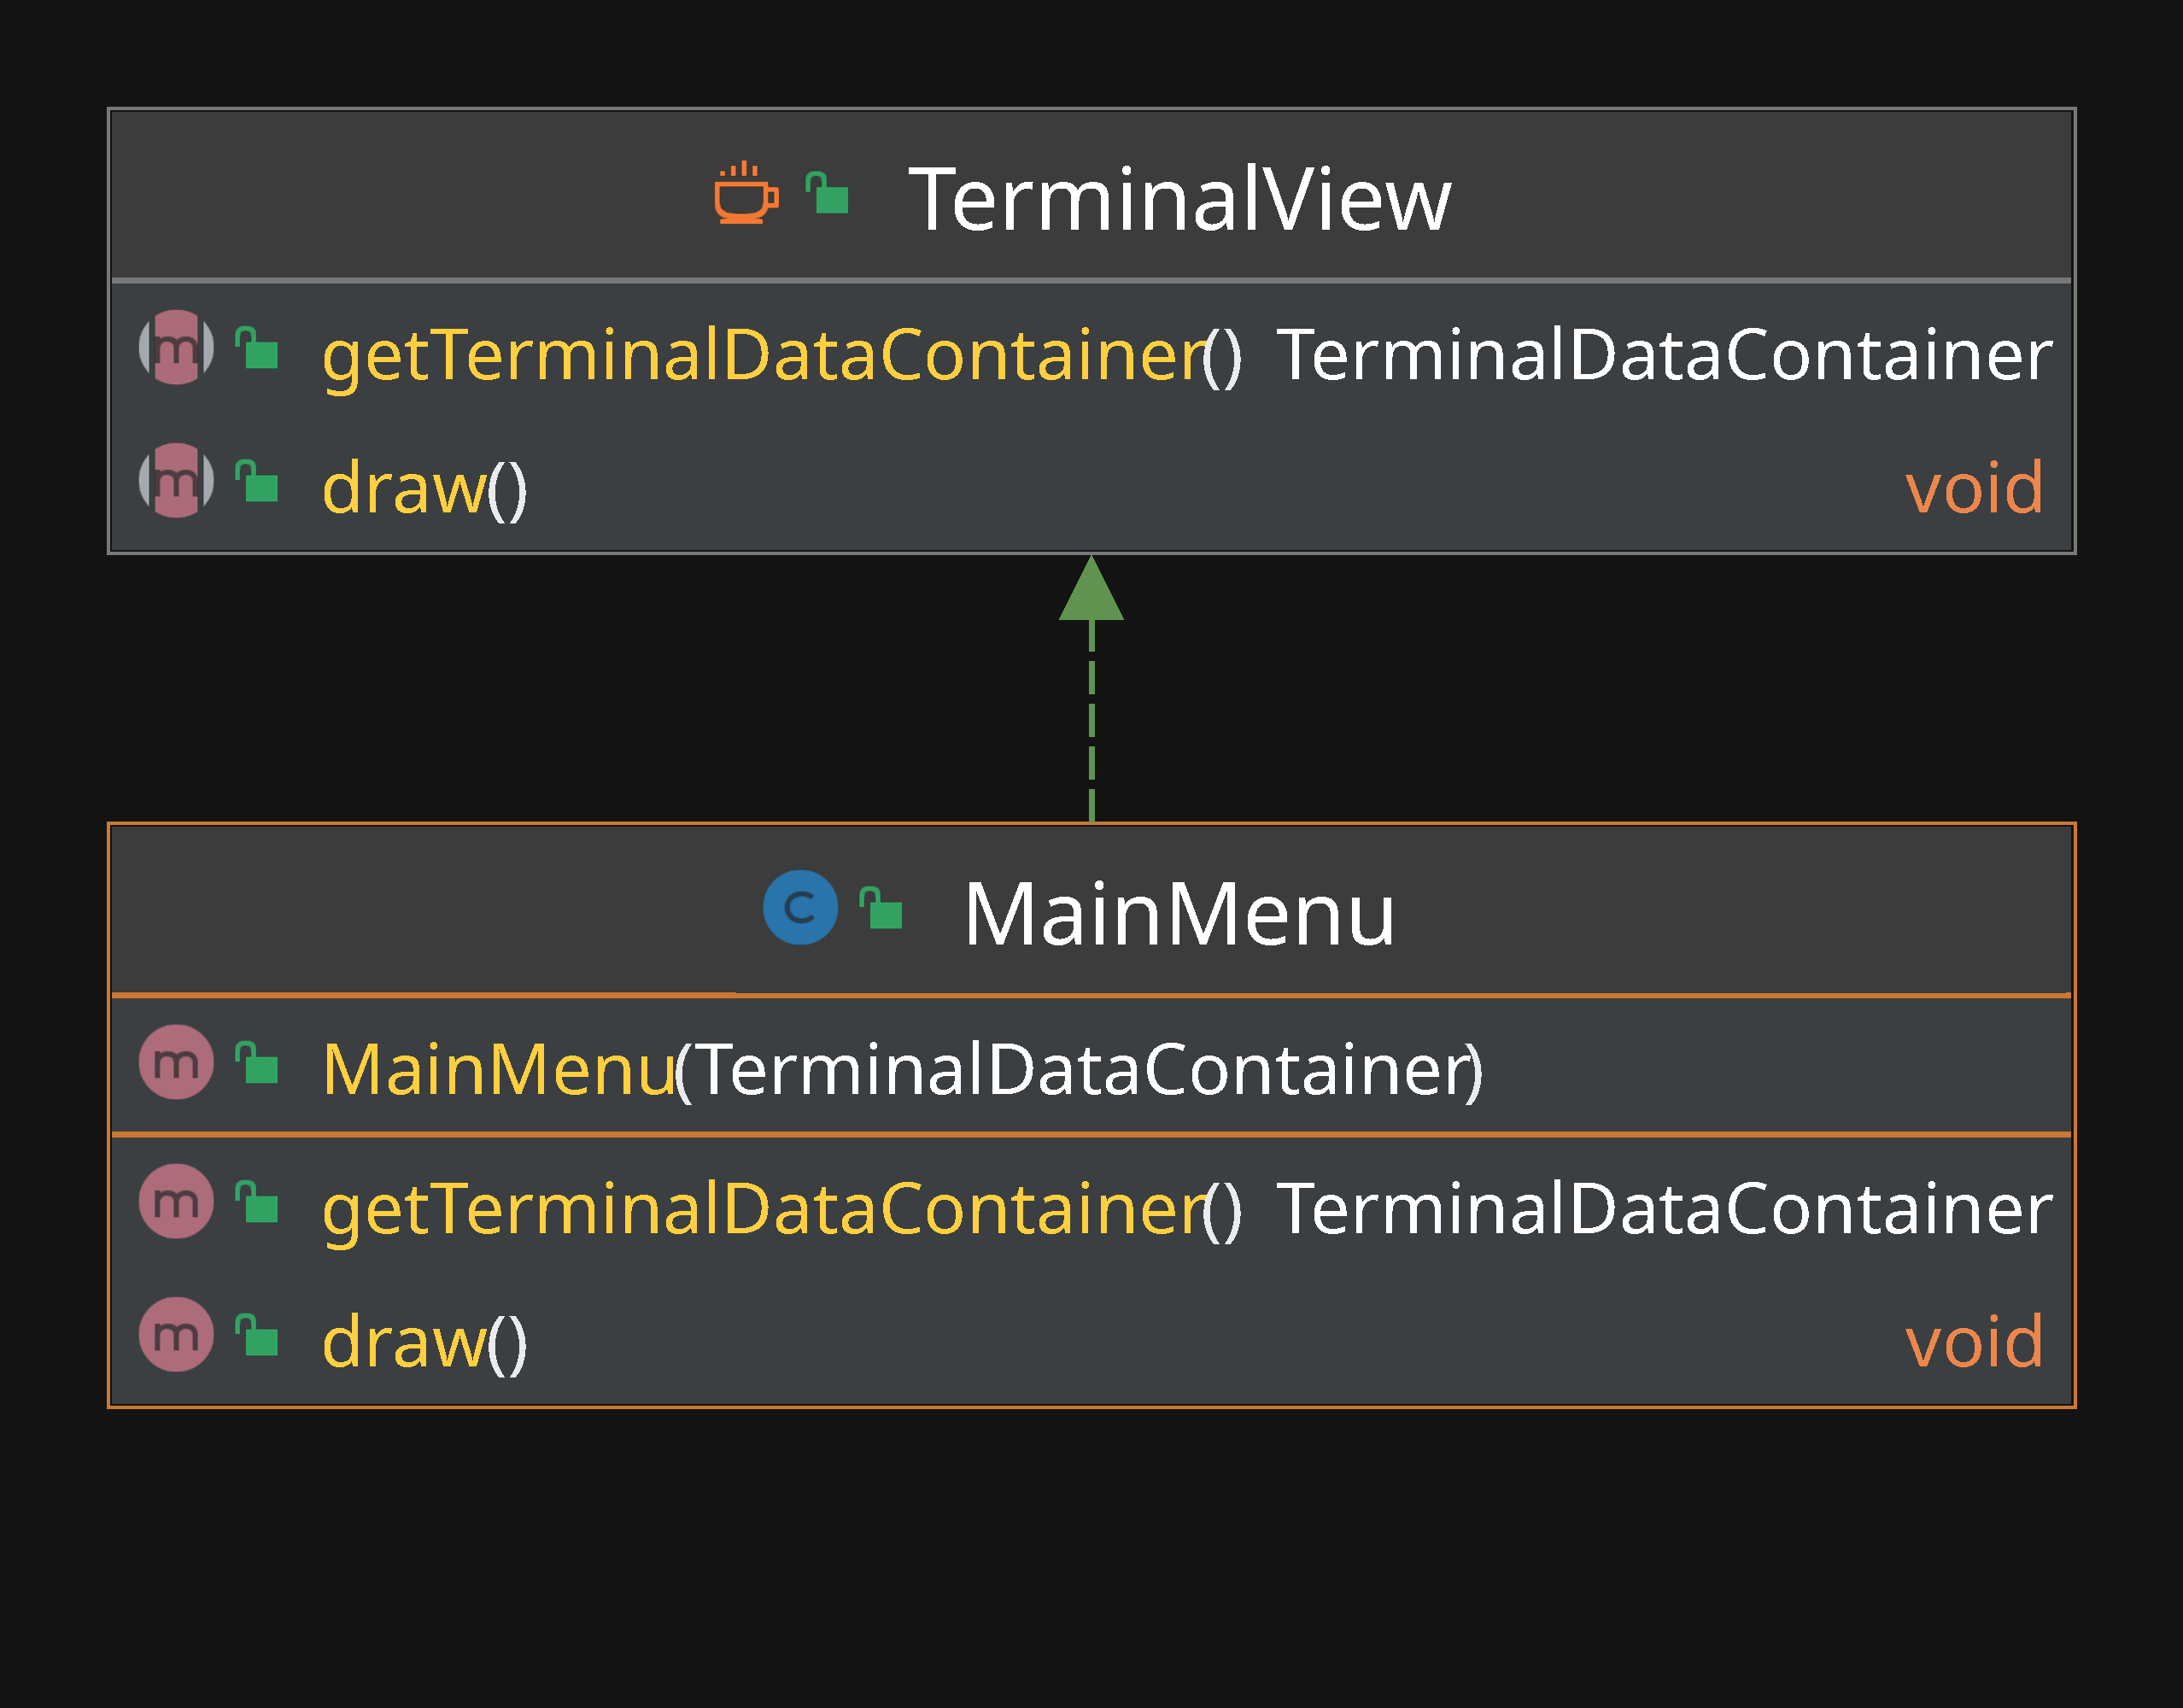
\includegraphics[width=0.5\textwidth]{Bilder/MainMenu.pdf}
	\caption{UML MainMenu}
	\label{fig:MainMenu}
\end{figure}

Die Klasse \texttt{MainMenu} liegt in der Plugin Schicht, da sie Teil des User Interfaces ist. Sie stellt den Einstiegspunkt der Nutzer Interaktion dar und stellt alle Möglichkeiten und Navigationspunkte dem User dar. Da die Implementierung des User Interfaces Framework spezifisch, bzw. Gerät spezifisch ist, gehört diese Klasse klar in die Plugin Schicht der Clean Architecture. Abbildung \ref{fig:MainMenu} zeigt das UML der Klasse.

\subsection{Domain: Weapon}
\begin{figure}[H]
	\centering
	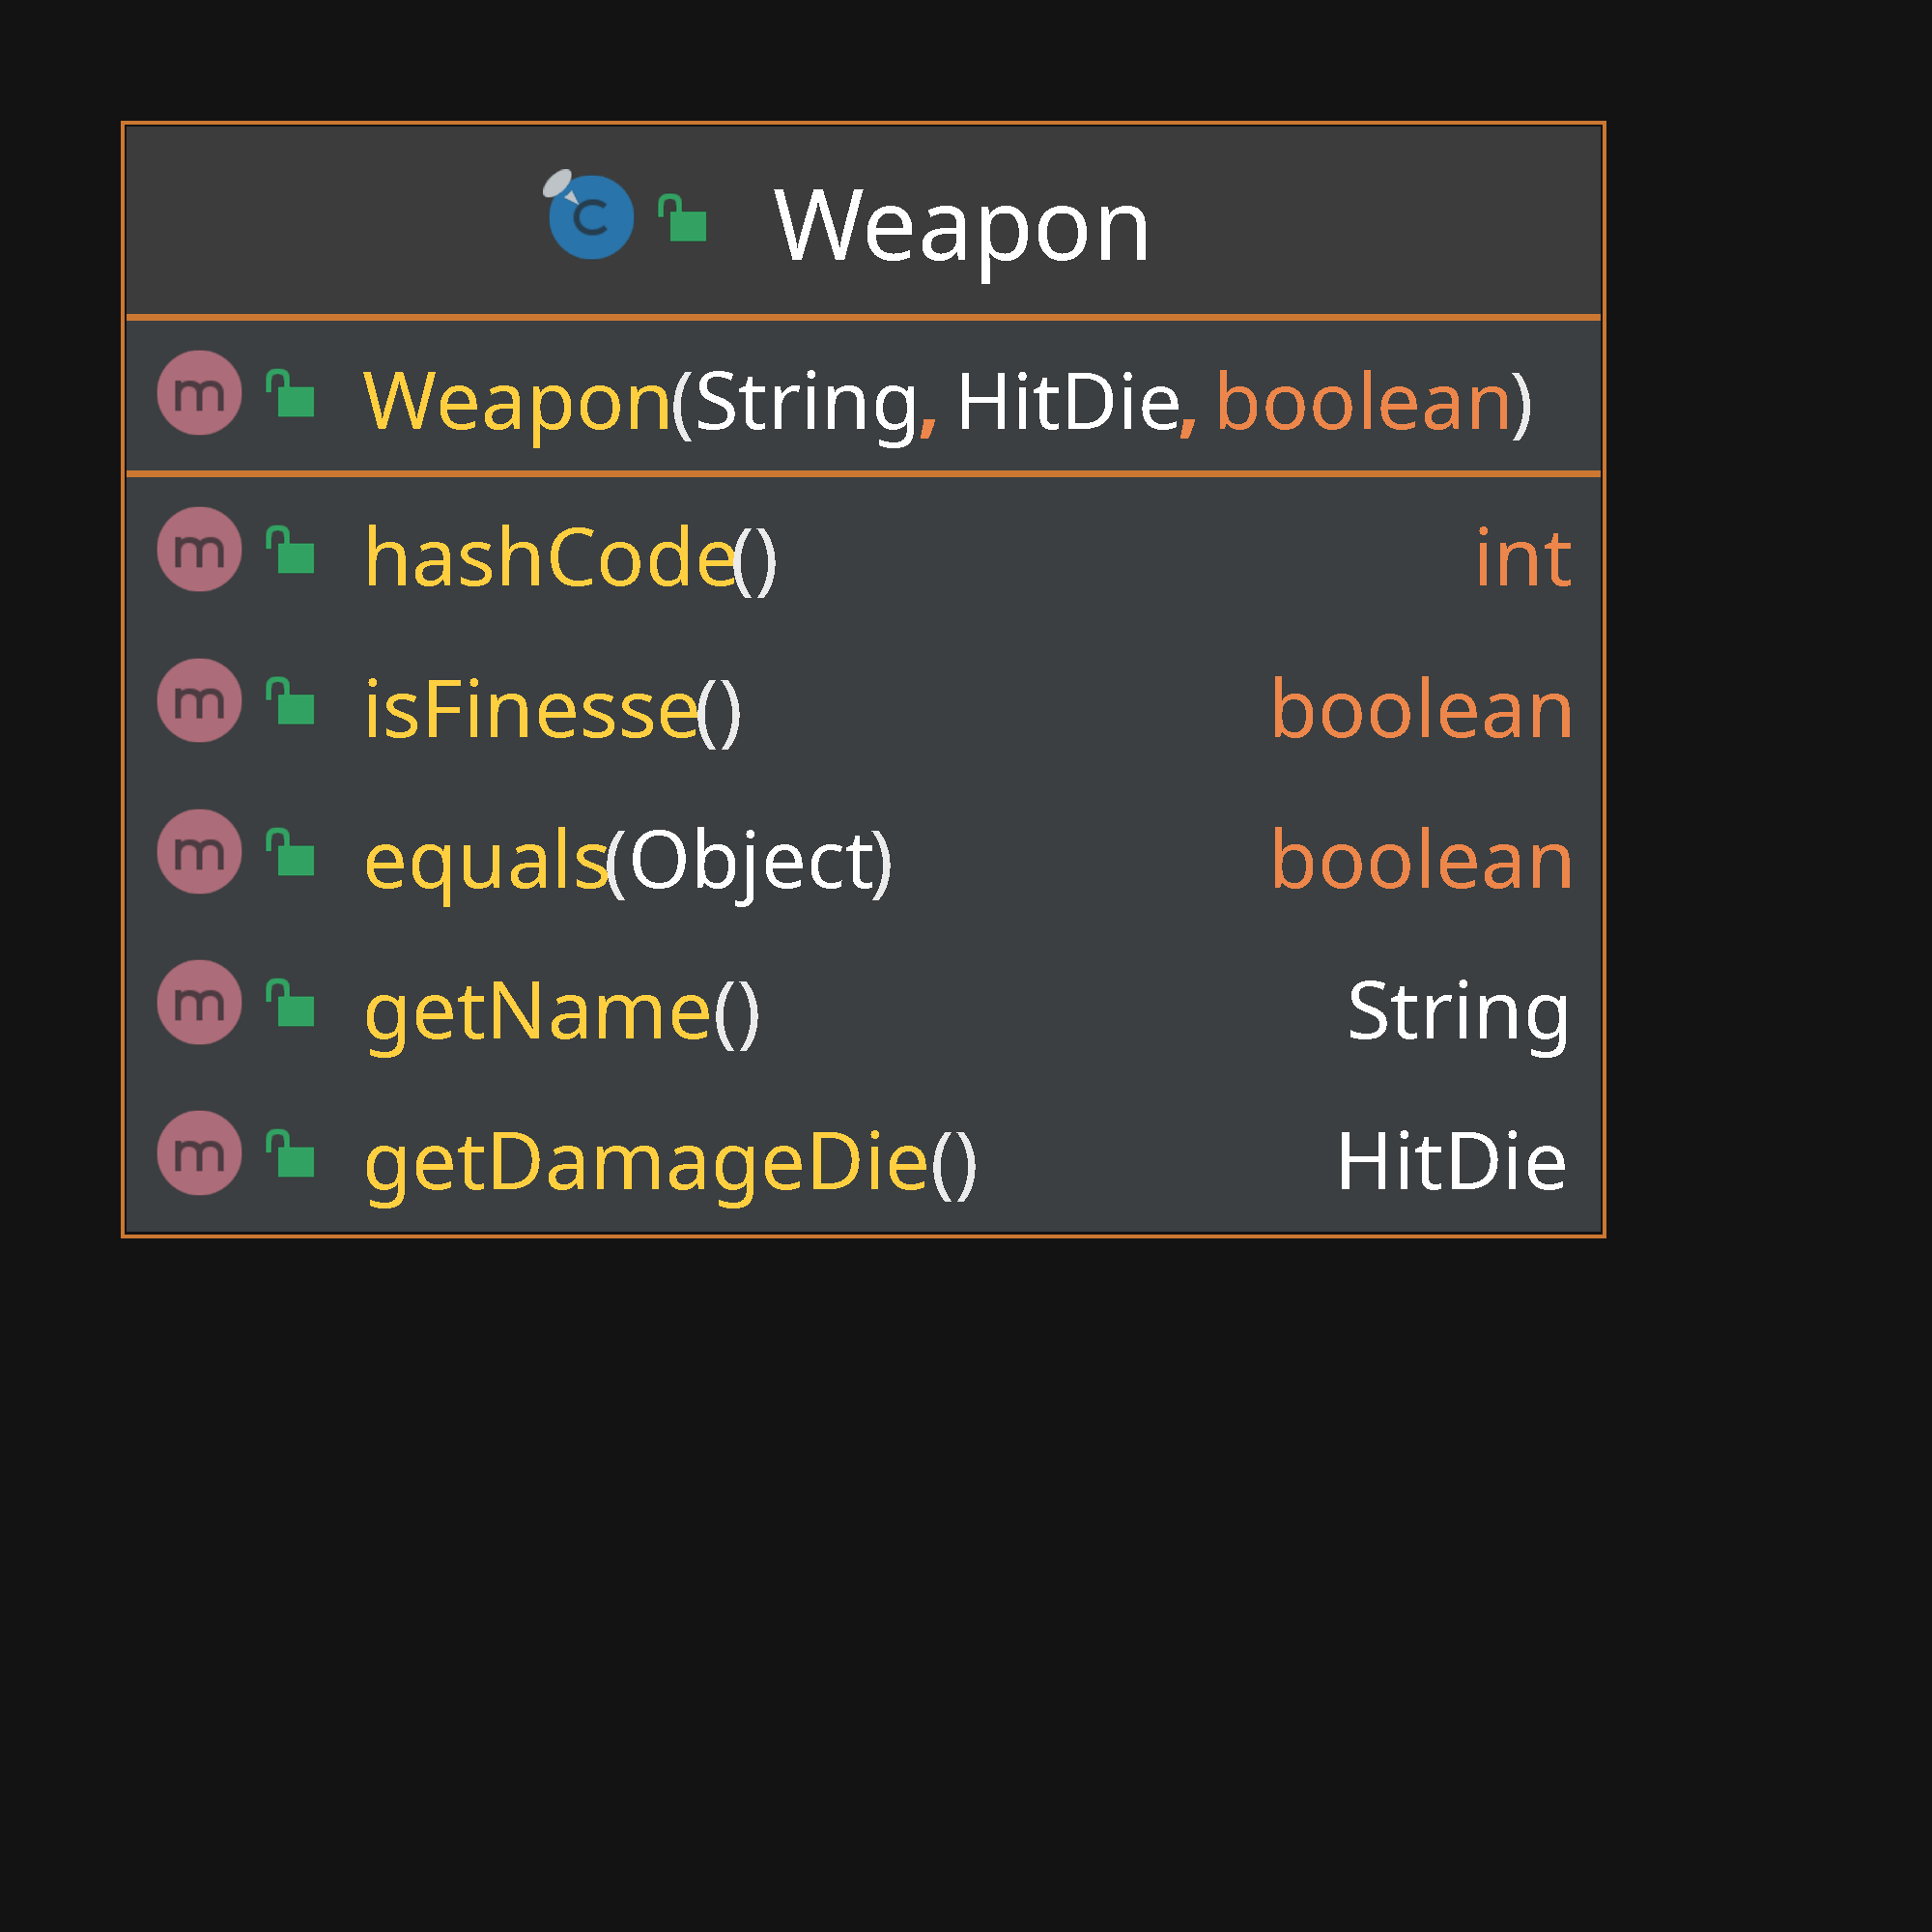
\includegraphics[width=0.5\textwidth]{Bilder/Weapon.pdf}
	\caption{UML Weapon}
	\label{fig:Weapon}
\end{figure}
Die Klasse Weapon Modelliert eine Waffe aus D\&D 5e. Sie enthält ausschließlich Daten und modelliert einen wichtigen Teil der Anwendungsdomäne. Somit ist sie klar in die Domain Schicht der Clean Architecture einzuordnen.

\chapter{SOLID}

\section{Analyse Single-Responsibility-Principle (SRP)}
[jeweils eine Klasse als positives und negatives Beispiel für SRP;  jeweils UML der Klasse und Beschreibung der Aufgabe bzw. der Aufgaben und möglicher Lösungsweg des Negativ-Beispiels (inkl. UML)]
\subsection{Positiv-Beispiel}
\begin{figure}[H]
	\centering
	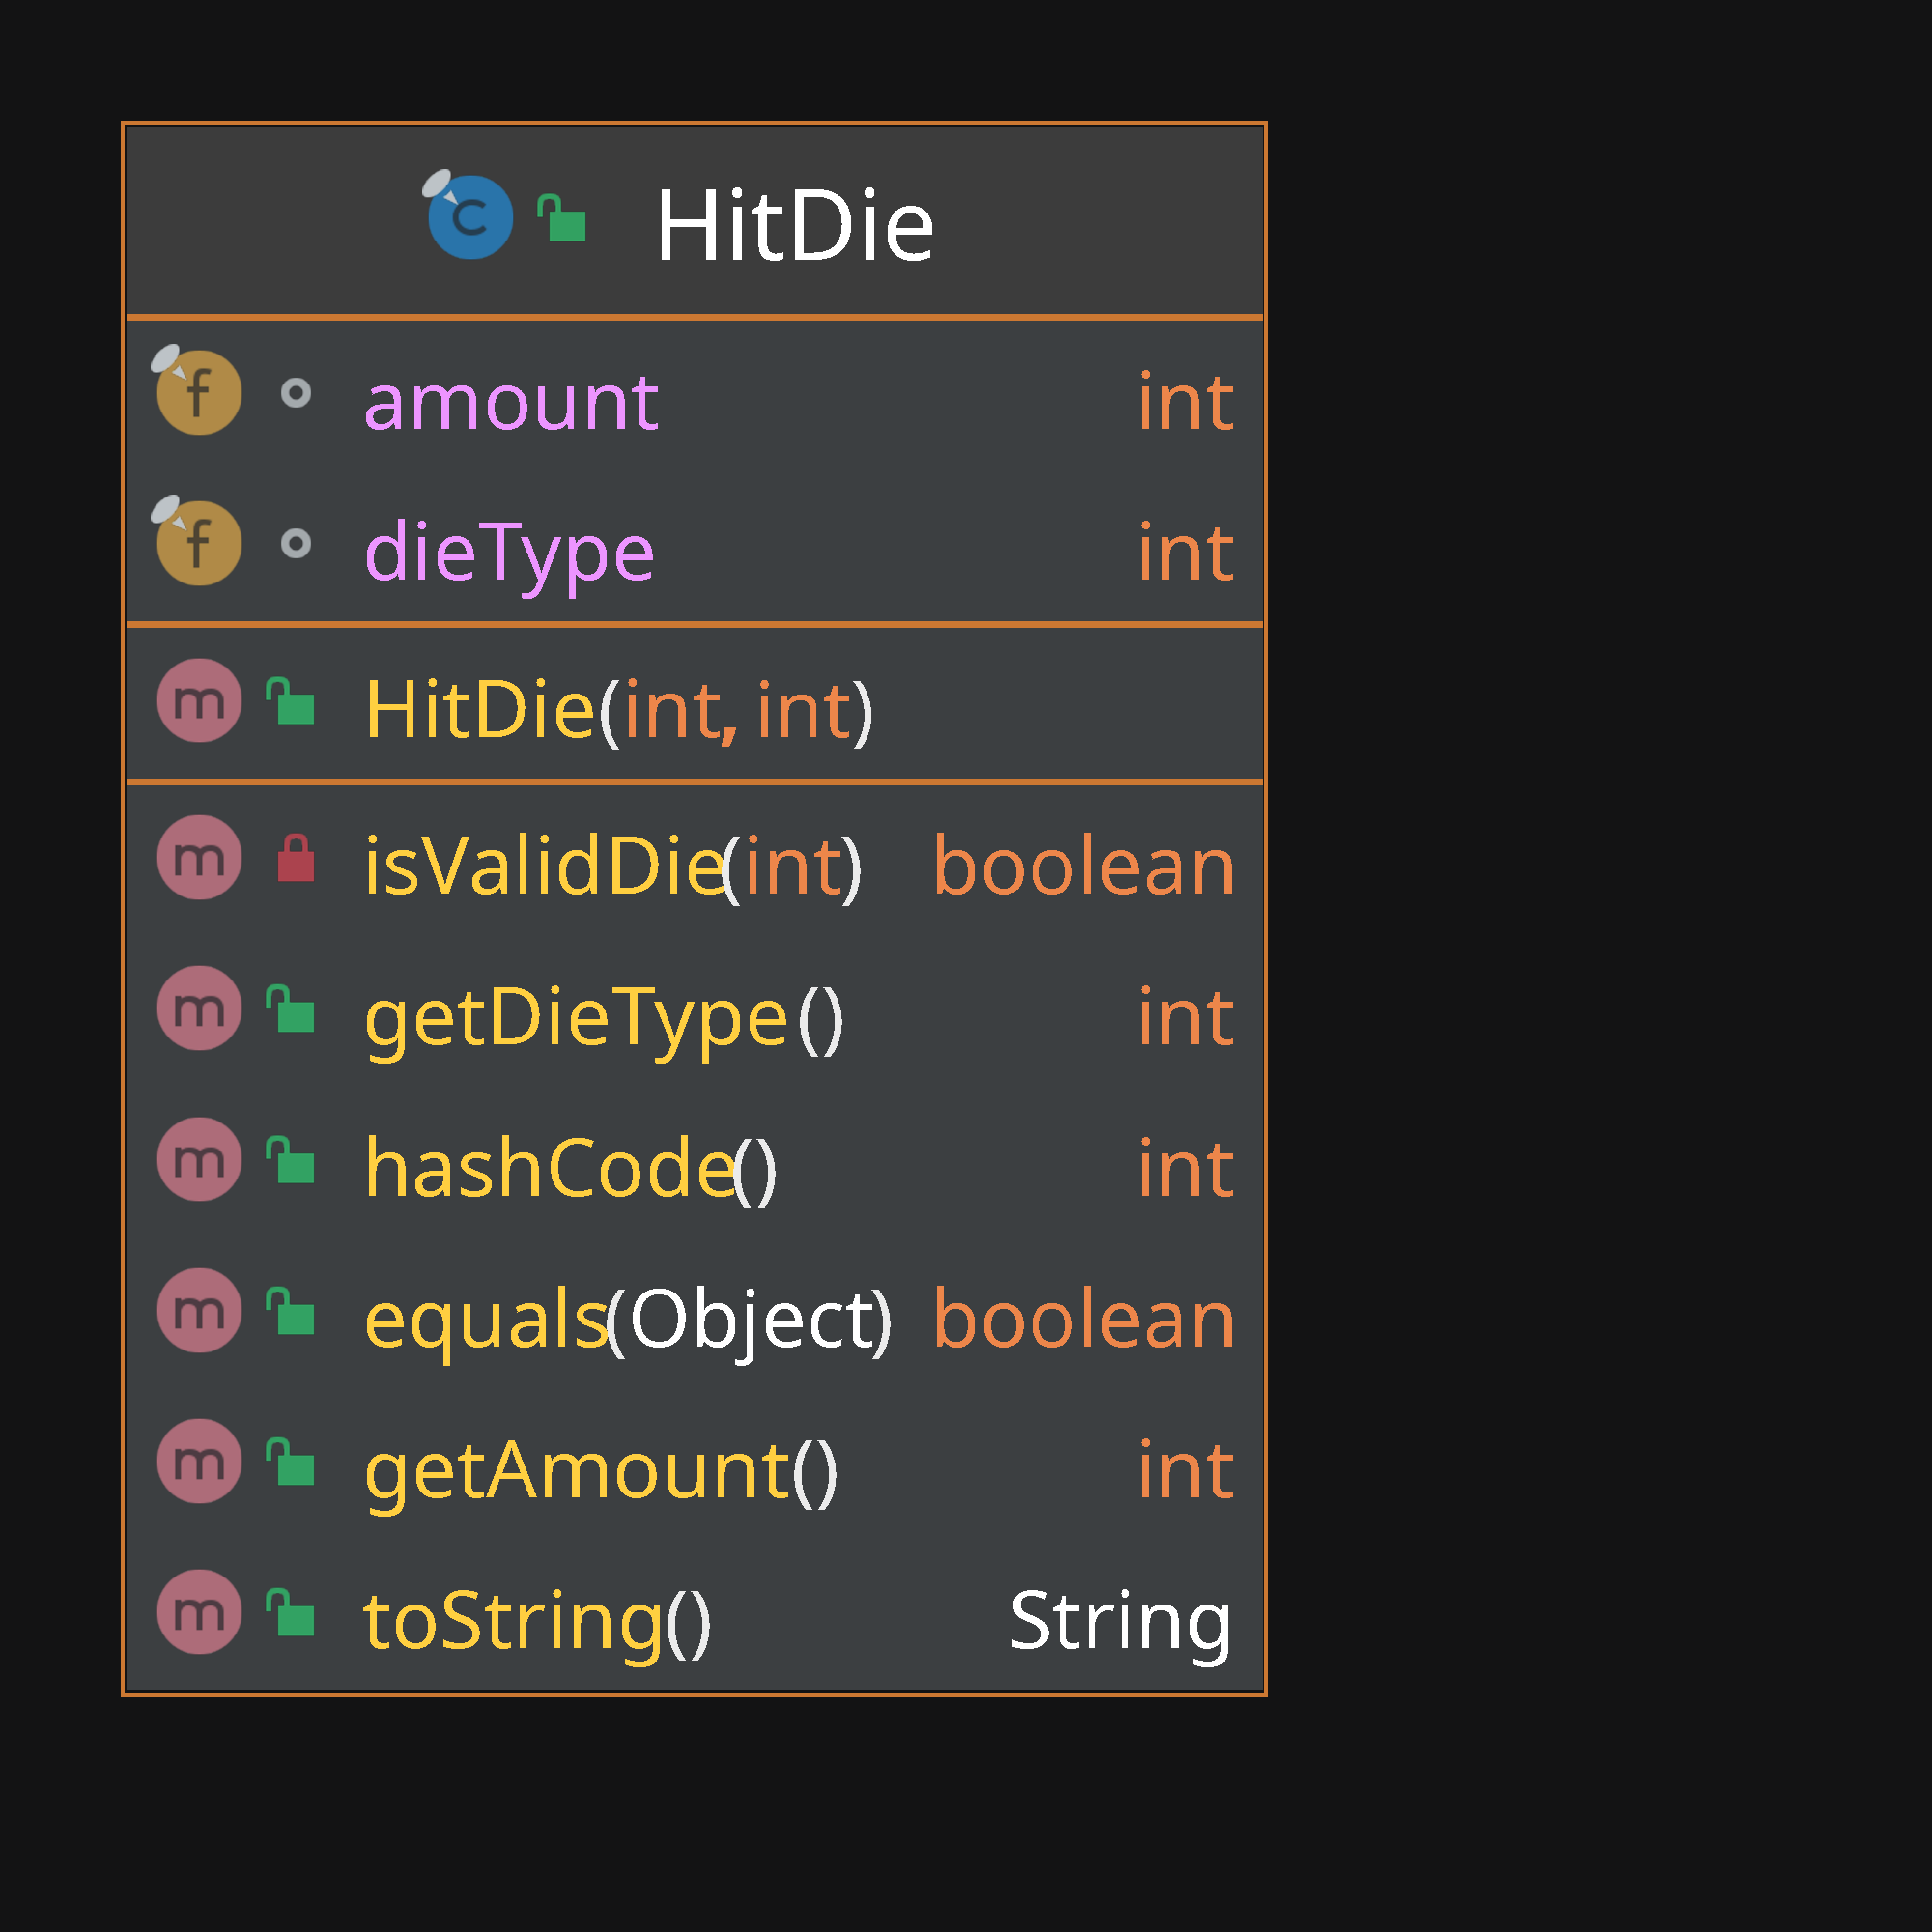
\includegraphics[width=0.4\textwidth]{Bilder/HitDie.pdf}
	\caption{UML der HitDie Klasse}
	\label{fig:HitDie-Solid}
\end{figure}
Abbildung \ref{fig:HitDie-Solid} zeigt das UML-Diagramm der \texttt{HitDie} Klasse. Sie hält das Single Responsibility Principle ein, da sie ausschließlich für die Repräsentation eines Würfels zuständig ist und keinerlei andere Funktionalität enthält.

\subsection{Negativ-Beispiel}
\begin{figure}[H]
	\centering
	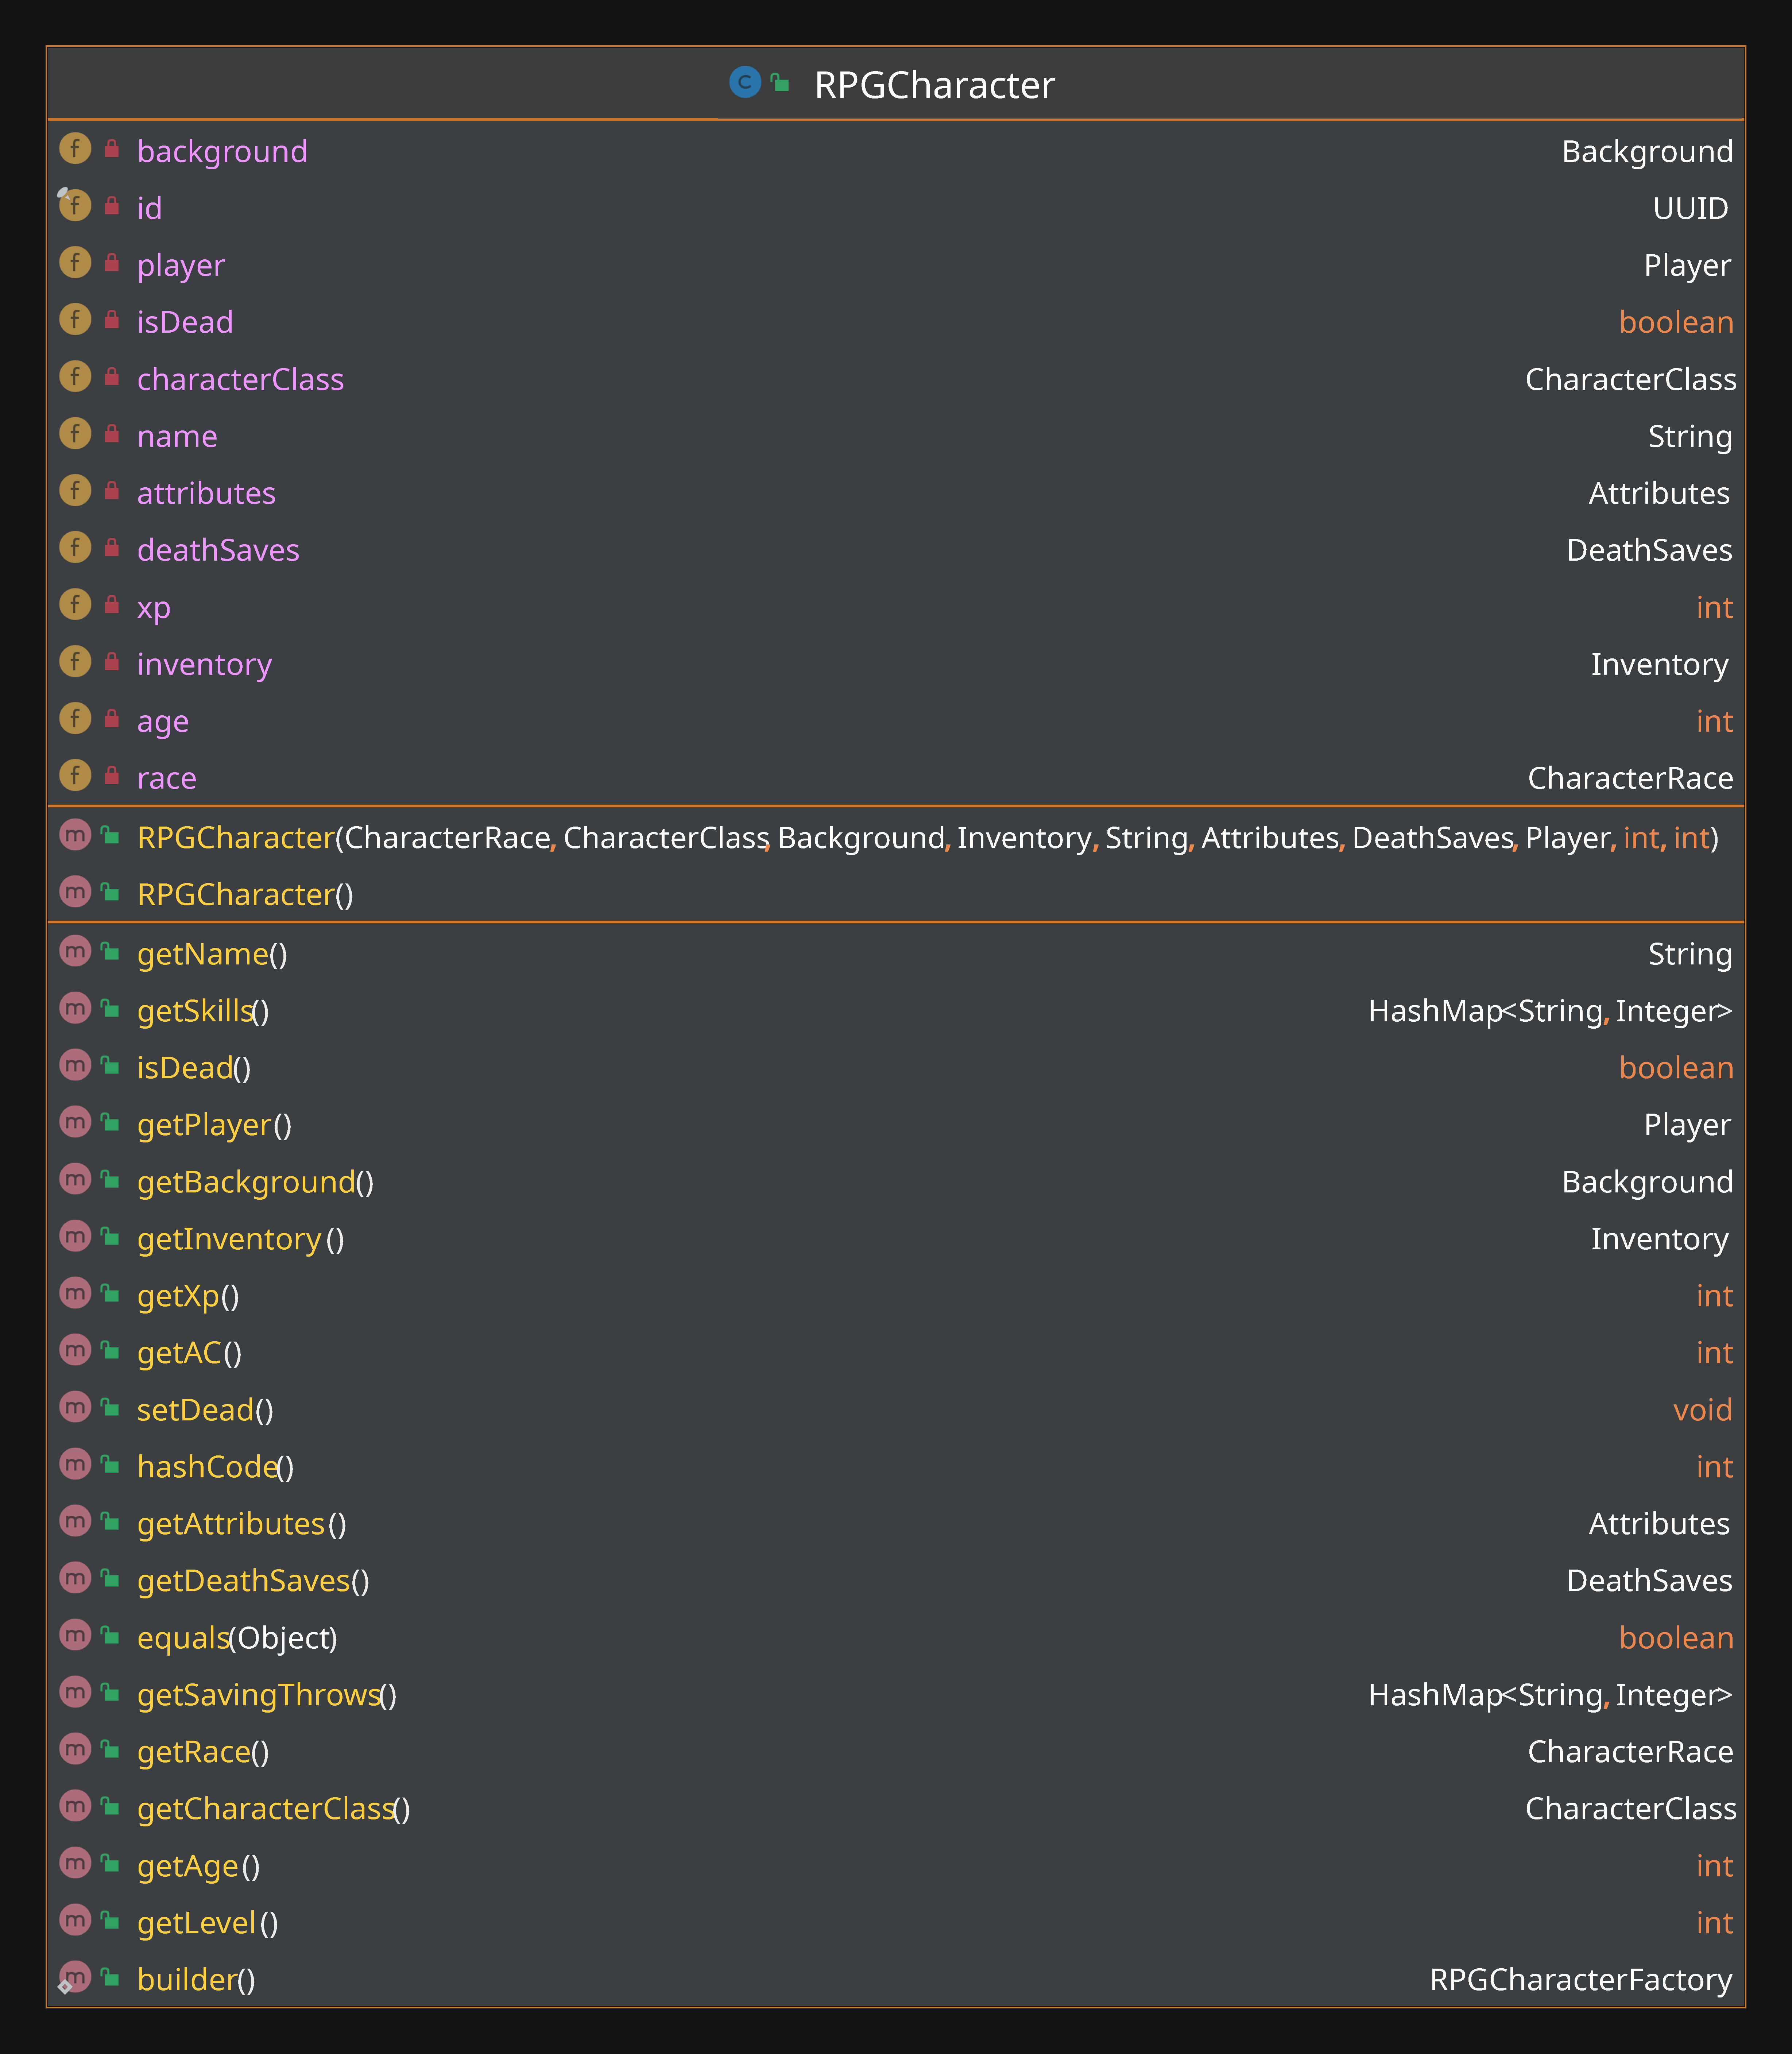
\includegraphics[width=0.4\textwidth]{Bilder/RPGCharacter.pdf}
	\caption{UML der RPGCharacter Klasse}
	\label{fig:RPG-Charadter}
\end{figure}
Die in Abbildung \ref{fig:RPG-Charadter} gezeigte \texttt{RPG-Character} Klasse hält das SRP nicht ein. Sie stellt nicht nur die verschiedenen Datenobjekte und Entitäten die ein Charakter hat zur Verfügung, sondern berechnet auch Status Werte wie z.B.: die ArmorClass (AC).  Daher wäre es sinnvoll diese Berechnung in eine eigene ArmorClass Klasse auszulagern, wie in Abbildung \ref{fig:RPG-CharadterSRP}.
\begin{figure}[H]
	\centering
	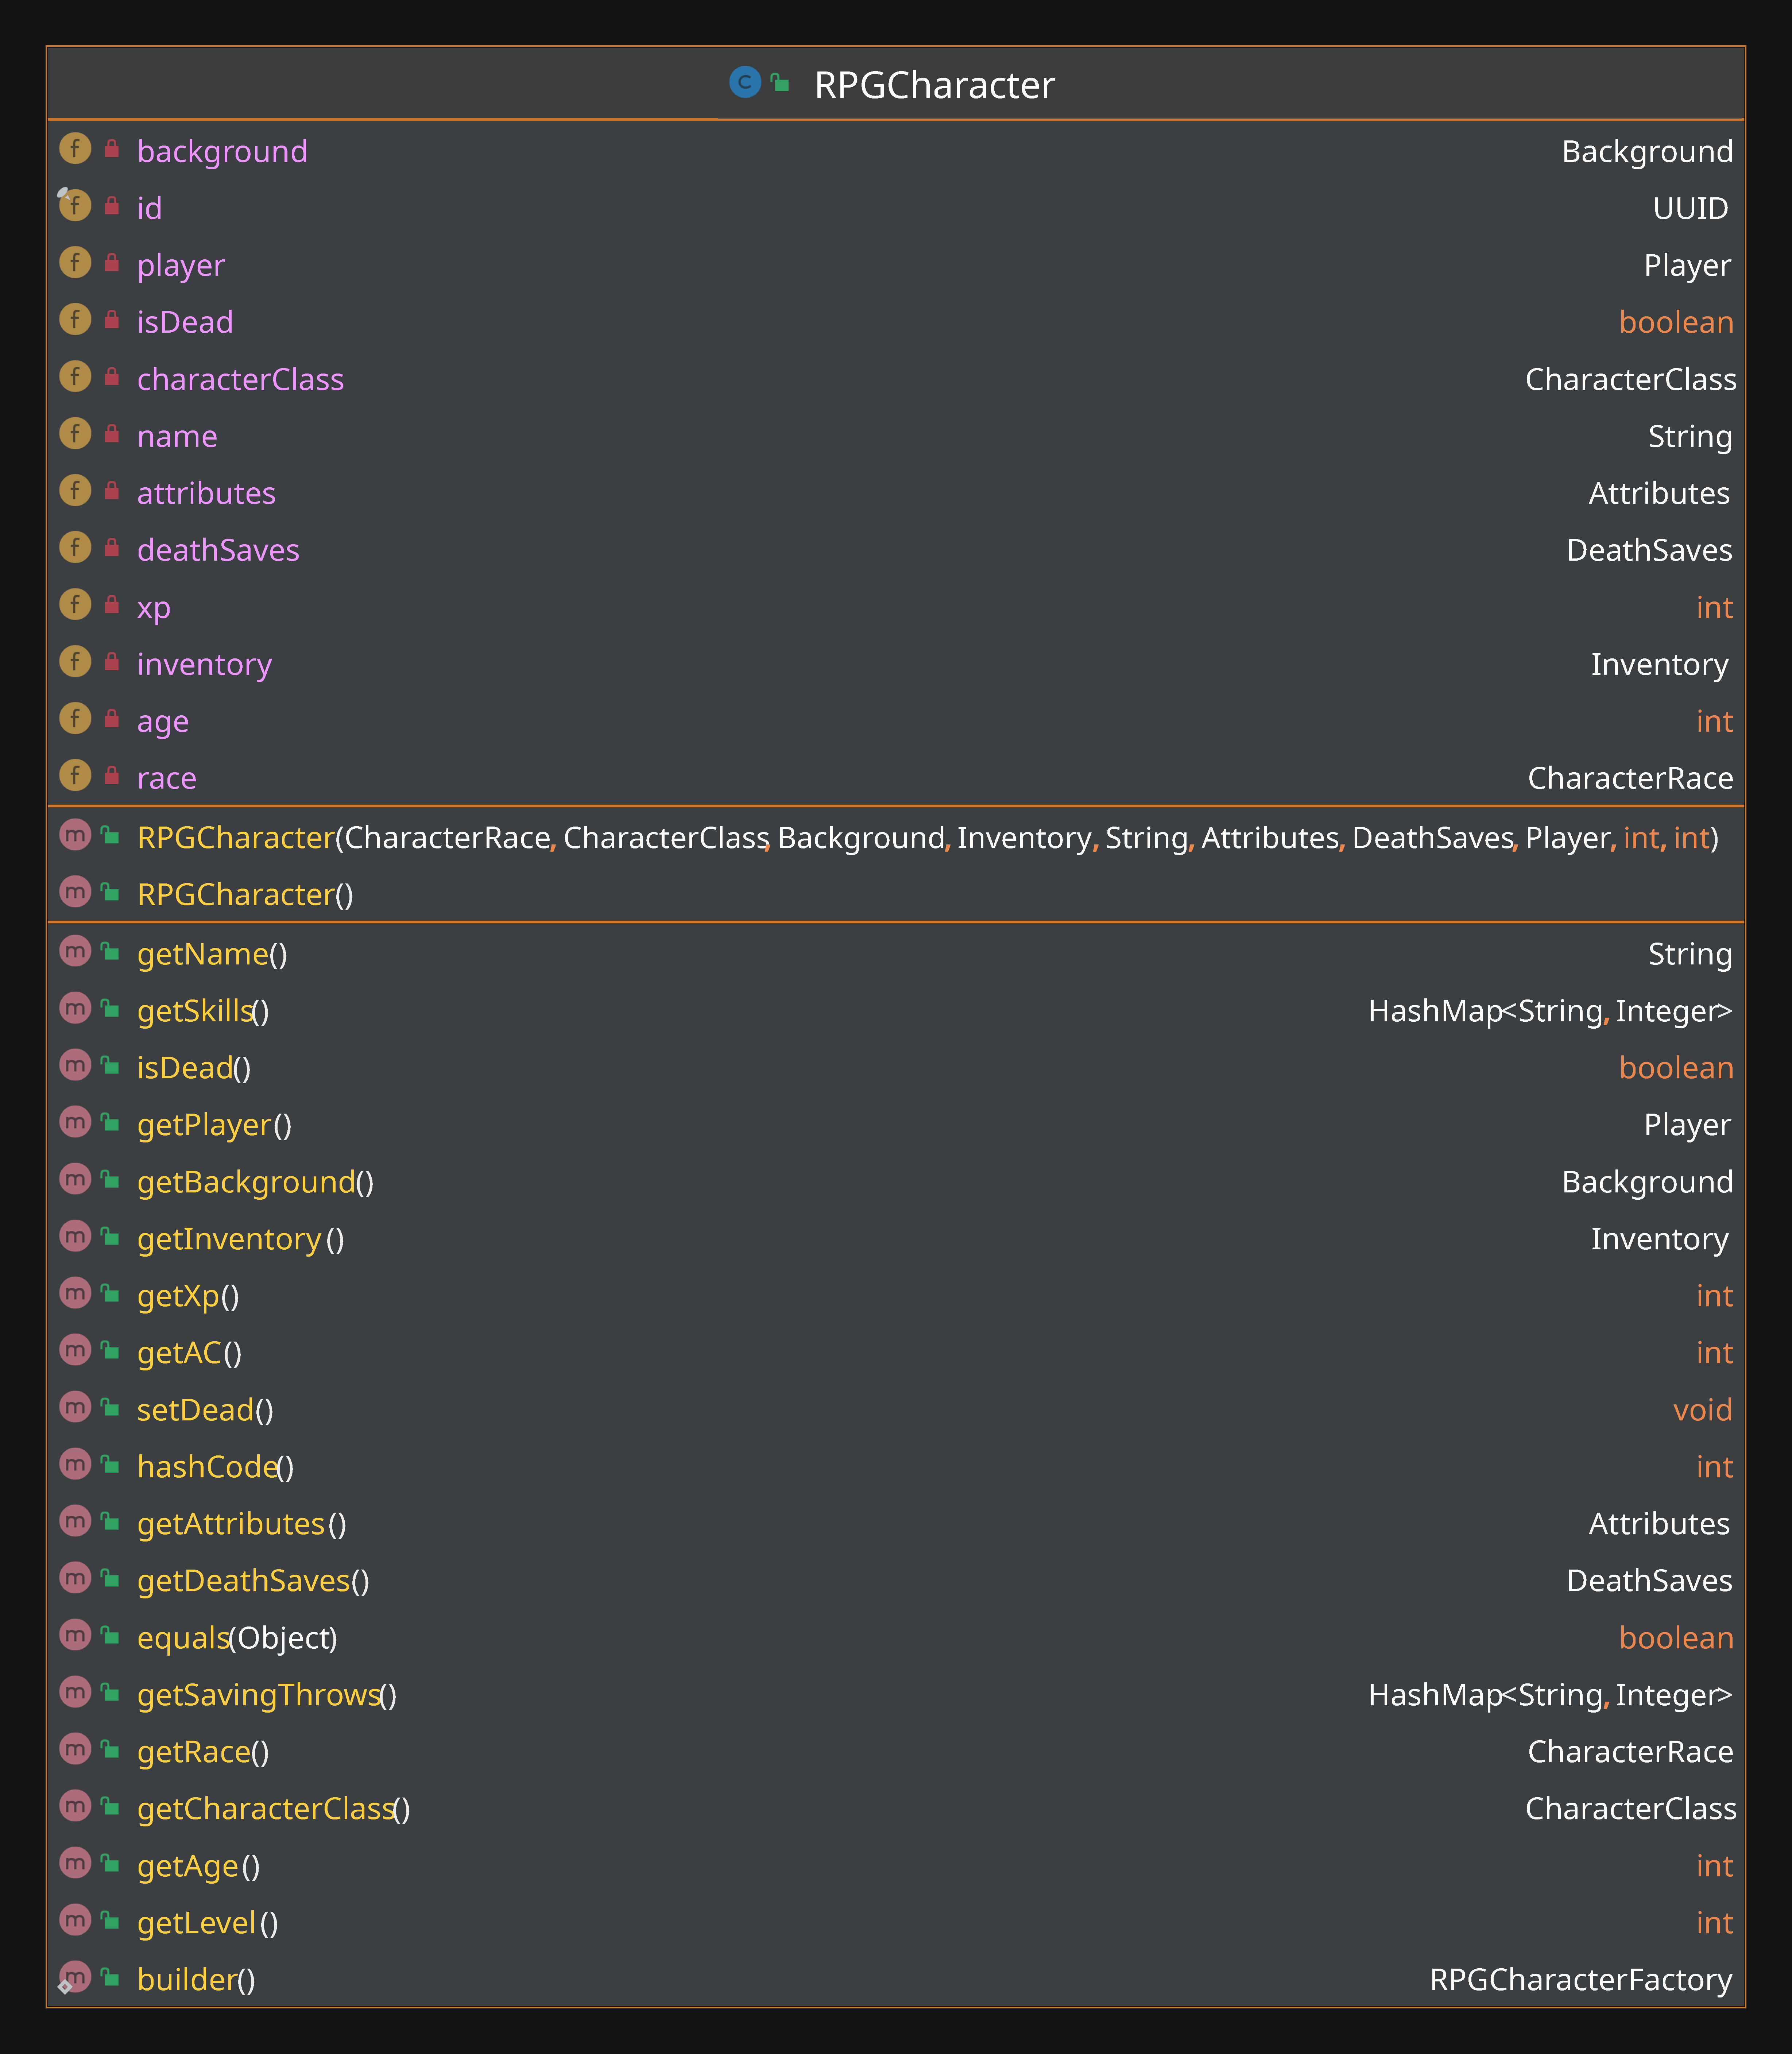
\includegraphics[width=0.4\textwidth]{Bilder/RPGCharacter.pdf}
		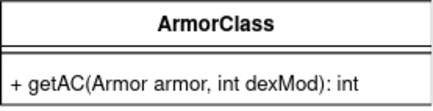
\includegraphics[width=0.4\textwidth]{Bilder/RPGCharacterSRP.drawio.pdf}
	\caption{UML der RPGCharacter Klasse und der theoretischen ArmorClass}
	\label{fig:RPG-CharadterSRP}
\end{figure}

\section{Analyse Open-Closed-Principle (OCP)}
\subsection{Positiv-Beispiel}
\begin{figure}[H]
	\centering
	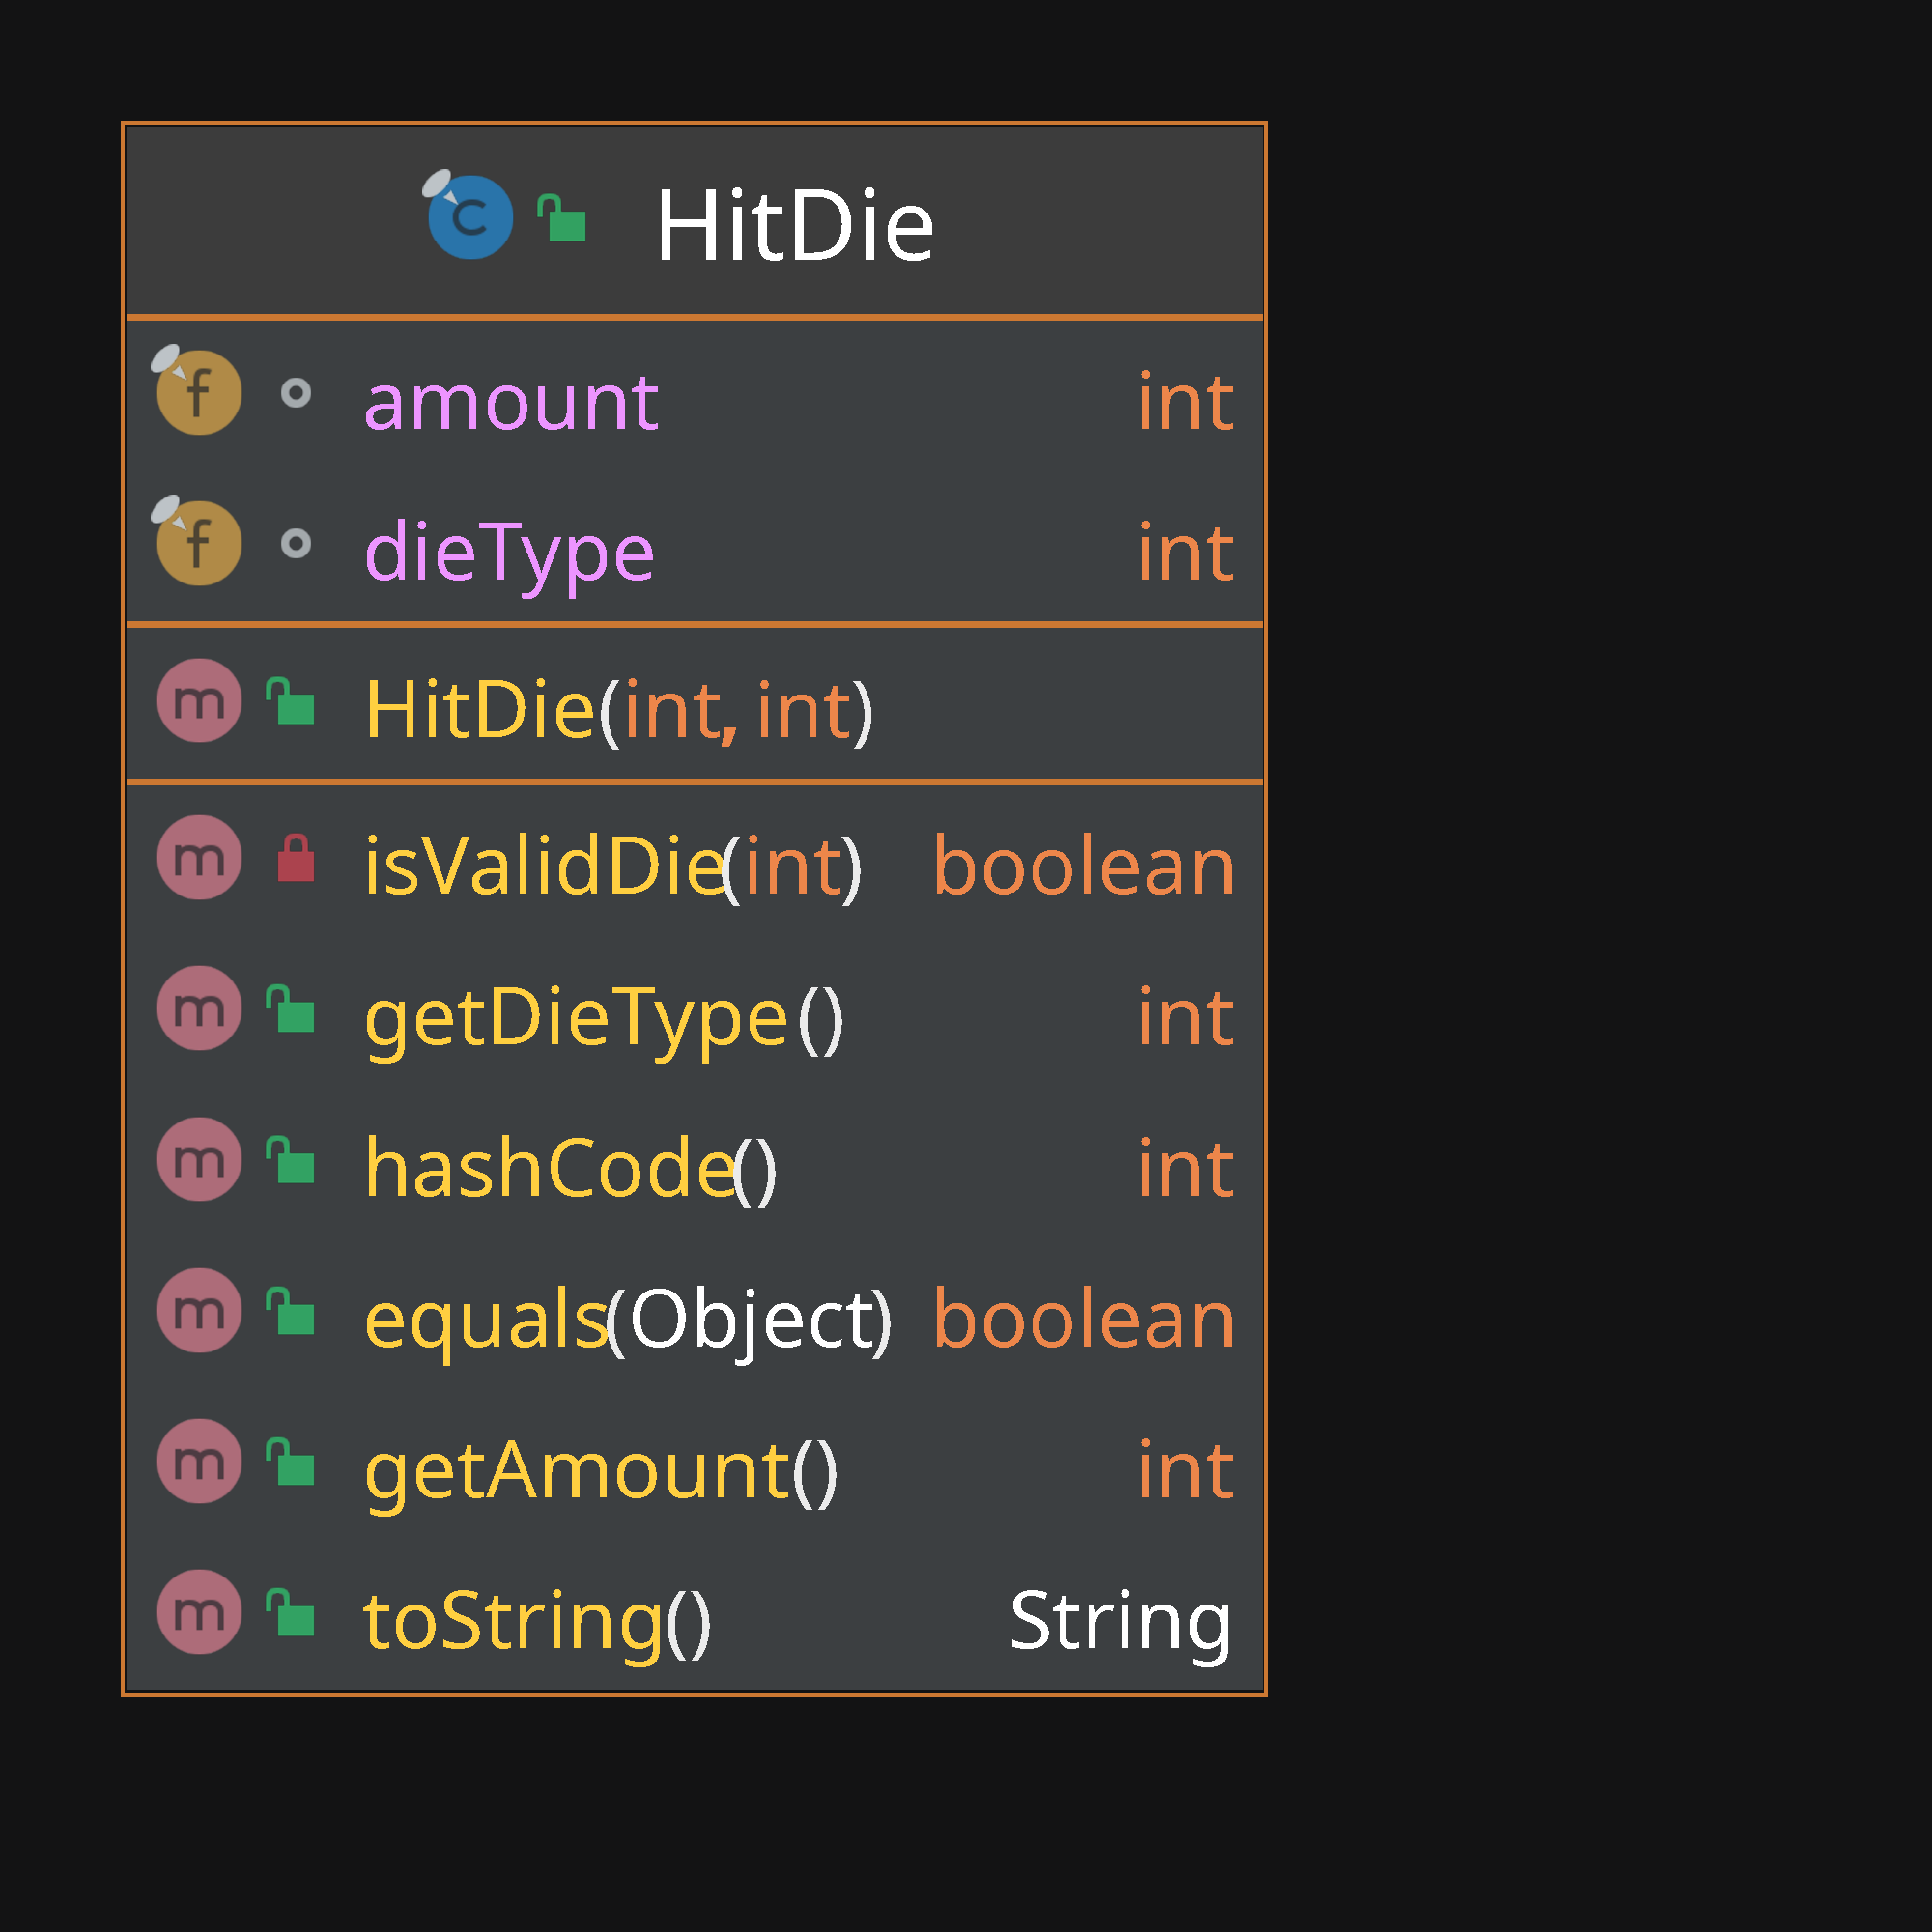
\includegraphics[width=0.4\textwidth]{Bilder/HitDie.pdf}
	\caption{UML der HitDie Klasse}
	\label{fig:HitDie-OCP}
\end{figure}
Die in Abbildung \ref{fig:HitDie-OCP} gezeigte Klasse \texttt{HitDie} hält das OCP ein, da sie alle Funktionen bereitstellt, die ein Würfel benötigt. Möchte man nun einen weiteren gültigen Würfel hinzufügen, muss nur diese Klasse angepasst werden und keine weiteren Änderungen im Projekt vorgenommen werden.
\subsection{Negativ-Beispiel}
Ich lasse an dieser Stelle das UML weg, da es keine Sinnvolle Aussagekraft hat. Die Klasse \texttt{SkillProficiencies} hält das OCP nicht ein, auch wenn sie eine Liste aller verfügbaren Skills enthält, muss man, wenn man einen neuen Skill hinzufügen möchte auch Änderungen in der \texttt{RPGCharacterClass} vornehmen. Da dort eine Hashmap zusammengebaut wird, die die tatsächlichen Werte enthalten. Somit liegt die Funktionalität der SkillProficiencies Klasse auf 2 Klassen aufgeteilt im Projekt und Änderungen und Modifikationen erfordern einen höheren Aufwand. Lösen könnte man dies, in dem man entweder in der Klasse SkillProficiencies eine neue Methode für die oben gennante Funktionalität anlegt, oder eine Klasse für die Skillwerte anlegt, die sich eine statische Liste aller validen Skills mit der SkillProficiencie Klasse teilt.

\section{Analyse Liskov-Substitution- (LSP), Interface-Segreggation- (ISP), Dependency-Inversion-Principle (DIP)}
\subsection{Positiv-Beispiel DIP}
\begin{figure}[H]
	\centering
	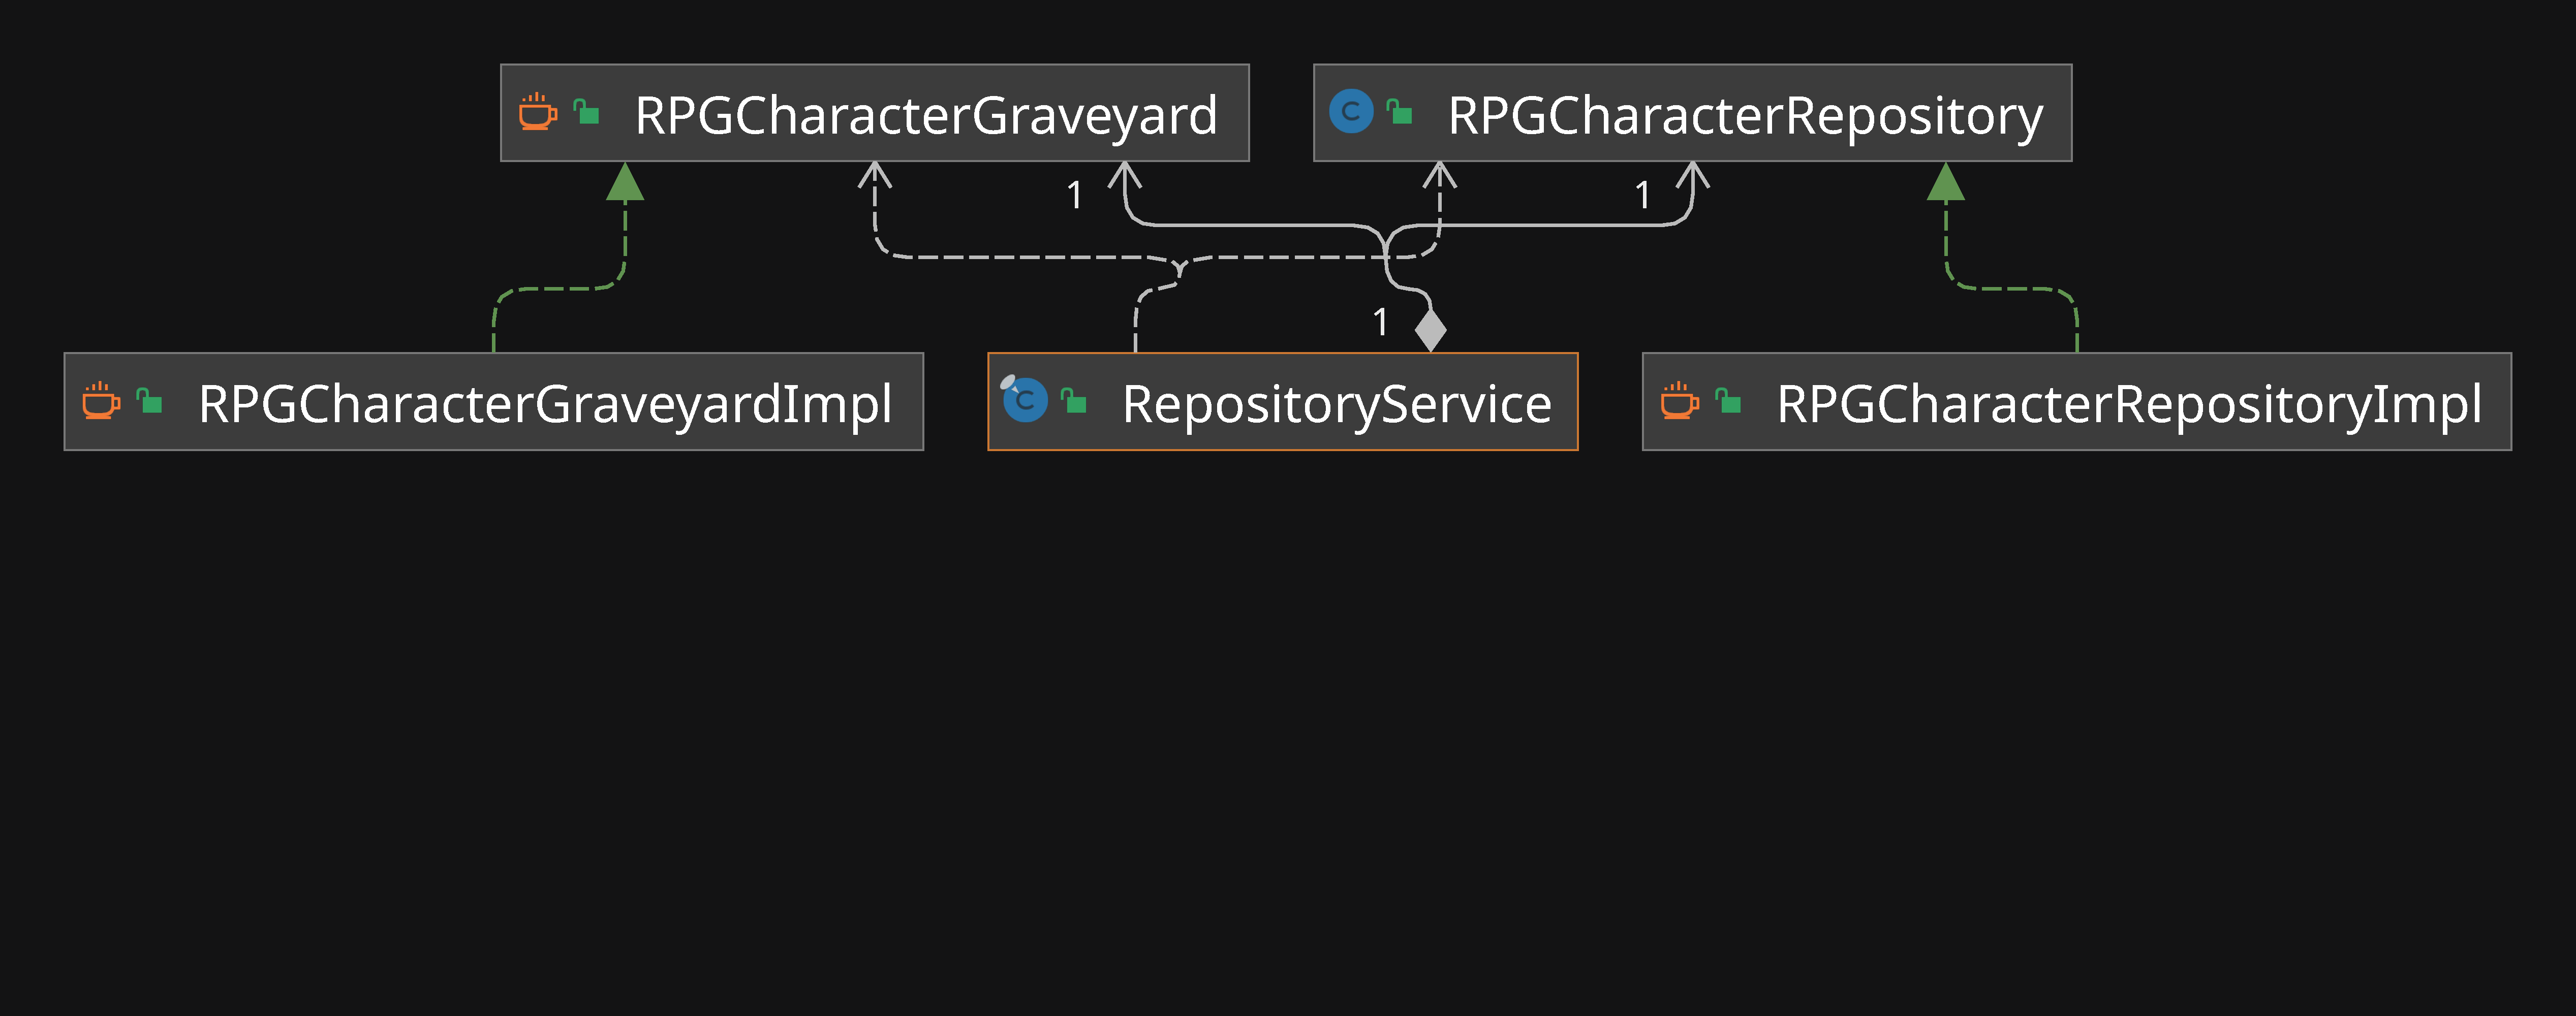
\includegraphics[width=0.6\textwidth]{Bilder/RepositoryService-DIP.pdf}
	\caption{UML der RepositoryService Klasse}
	\label{fig:repservdip}
\end{figure}
Der RepositoryService hält das DIP ein, da er ausschließlich von einer Abstraktion der Repositorys in Form der jeweiligen Interfaces Abhängig ist, nicht aber von der Klasse und der Implementation selbst. Somit kann die Implementation jederzeit geändert werden, ohne das der RepositoryService verändert werden muss. 
- Repositorys
\subsection{Negativ-Beispiel}
\begin{figure}[H]
	\centering
	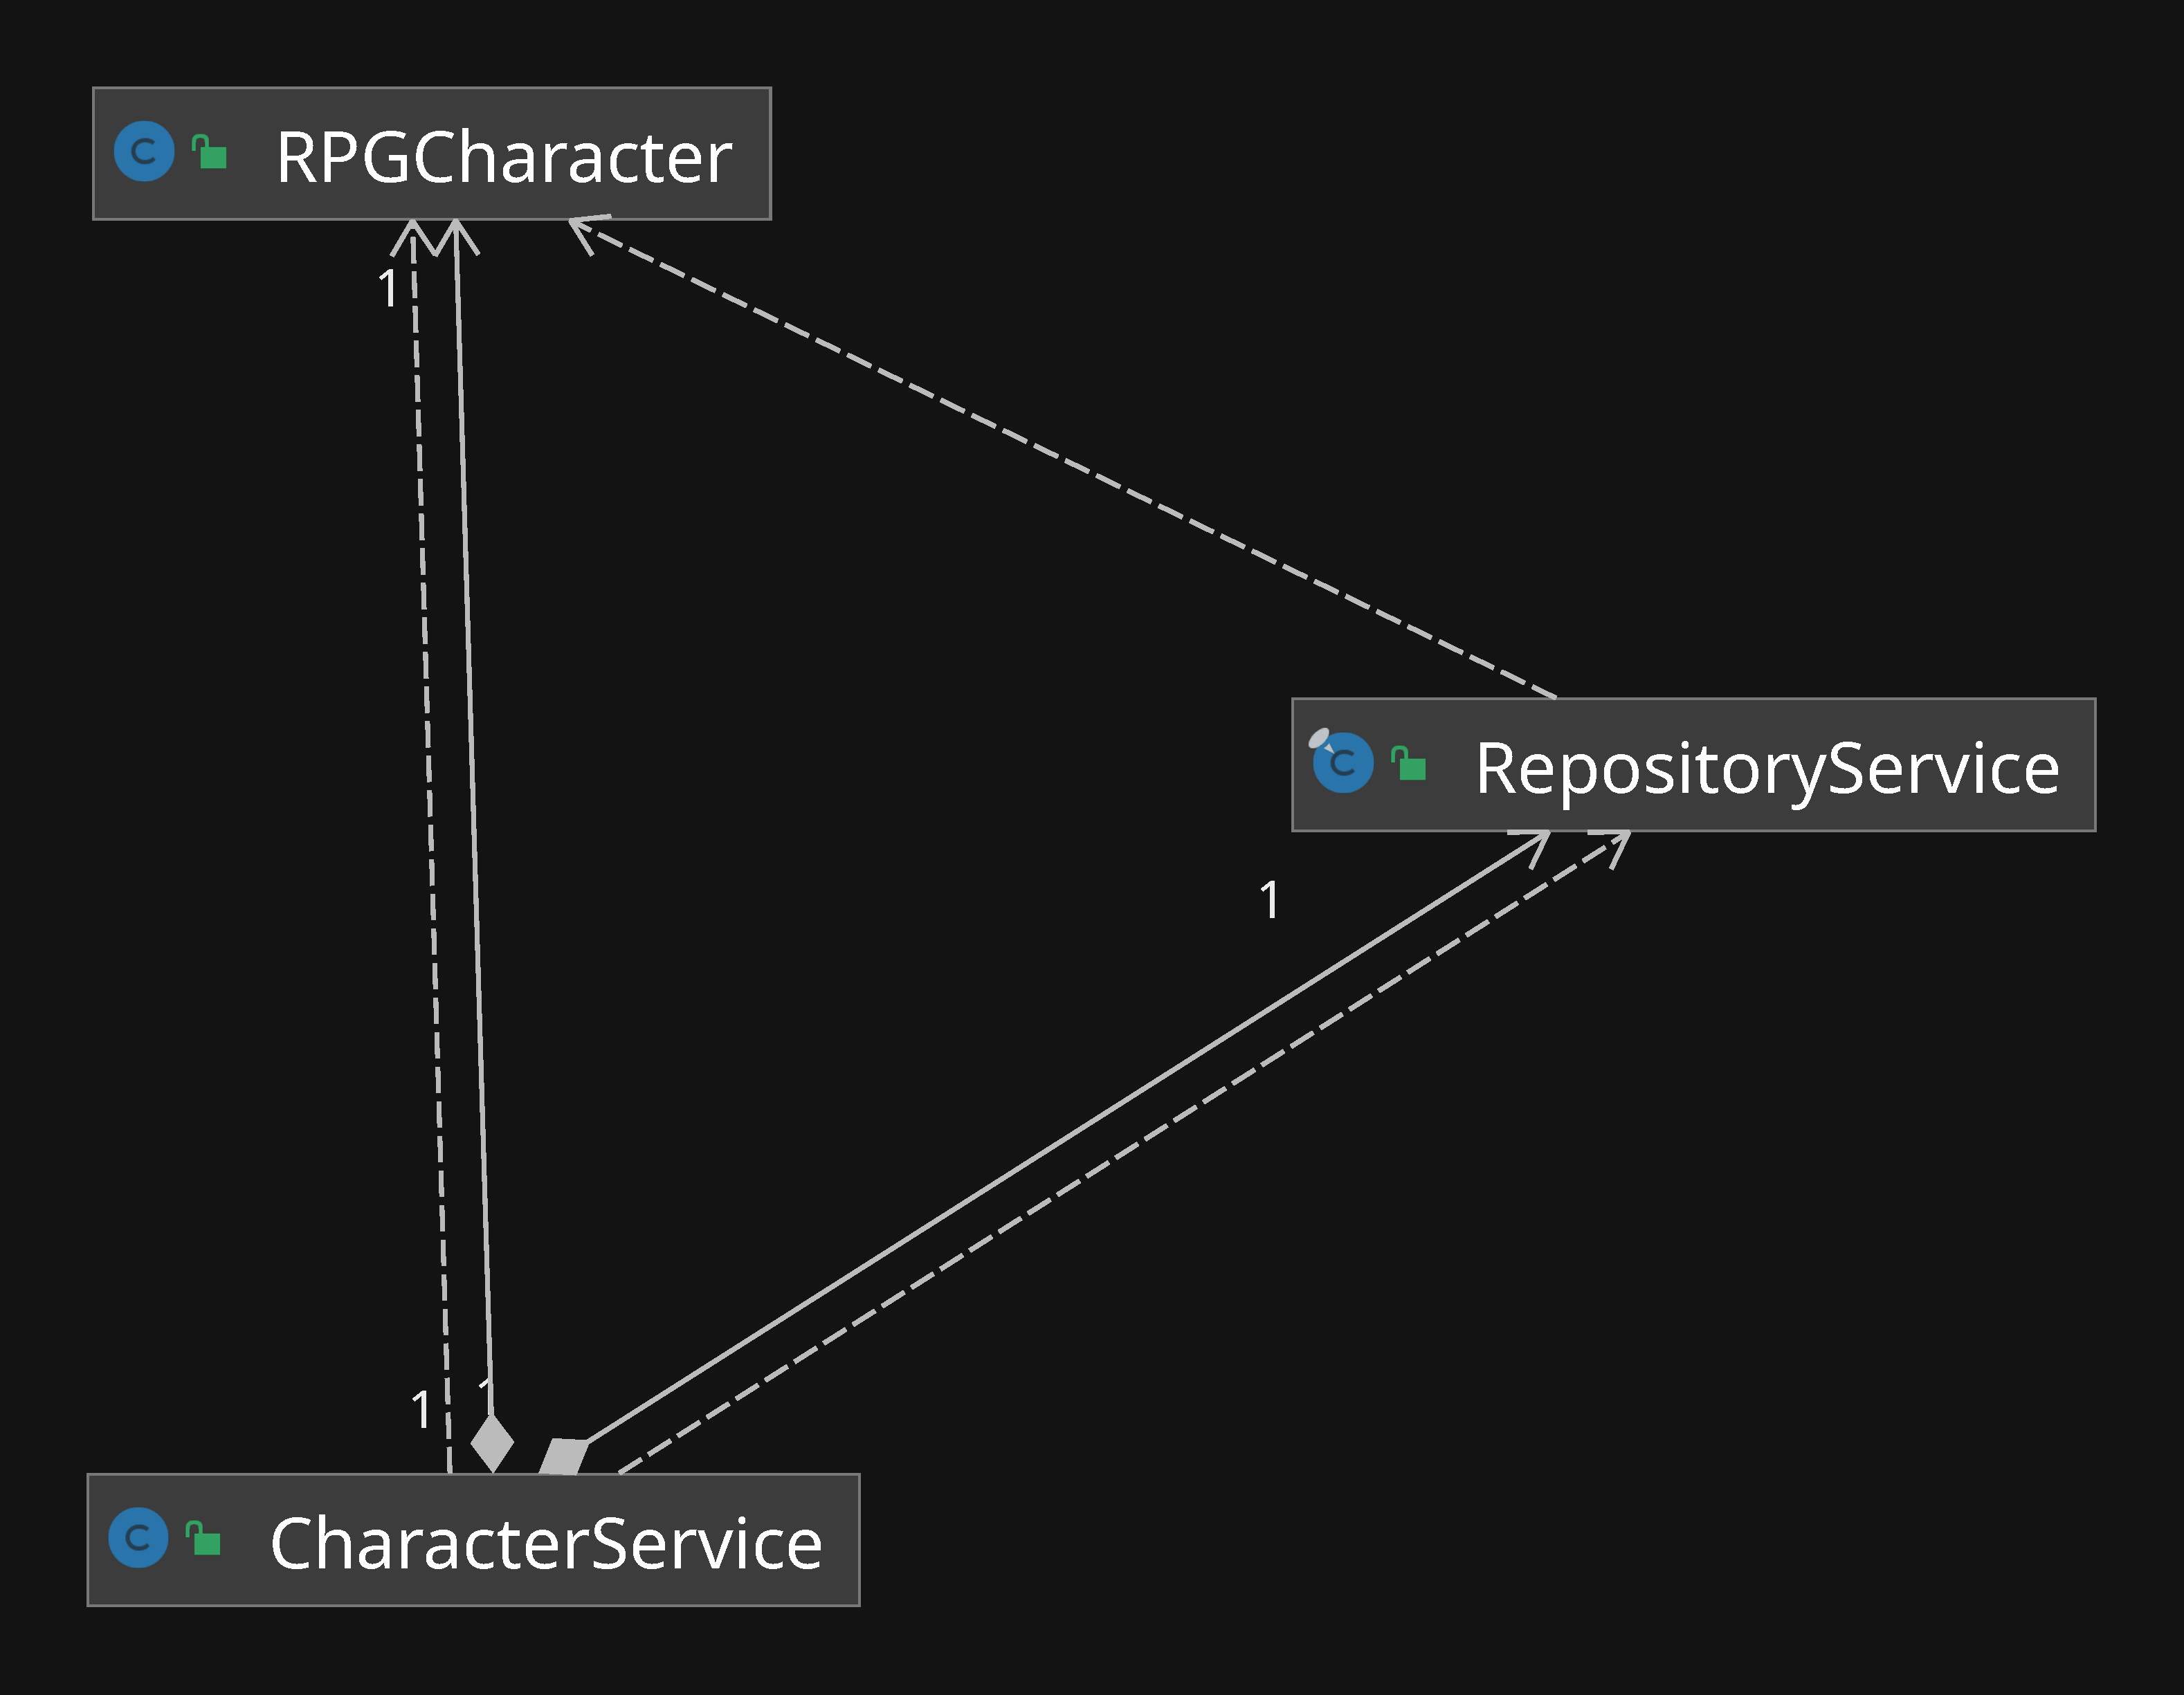
\includegraphics[width=0.6\textwidth]{Bilder/CharacterService-DIP.pdf}
	\caption{UML der CharacterService Klasse}
	\label{fig:characterServDip}
\end{figure}
Die Klasse CharacterService hält DIP wiederum nicht ein. Sie speichert direkt Verweise auf Objekte und ruft in allen Methoden, Methoden der gespeicherten Objekte sofort auf. Somit ist sie direkt Abhängig von den Objekten und nutzt keinerlei Abstraktionen.
\chapter{Weitere Prinzipien}

\section{Analyse GRASP: Geringe Kopplung}
[jeweils eine bis jetzt noch nicht behandelte Klasse als positives und negatives Beispiel geringer Kopplung; jeweils UML Diagramm mit zusammenspielenden Klassen, Aufgabenbeschreibung und Begründung für die Umsetzung der geringen Kopplung bzw. Beschreibung, wie die Kopplung aufgelöst werden kann]
\subsection{Positiv-Beispiel}
Gibt keines, da sich ein Listenerpattern im Projekt nicht angeboten hat.
\subsection{Negativ-Beispiel}
\begin{figure}[H]
	\centering
	\includegraphics[width=0.9\textwidth]{Bilder/RPGCharacter-kopplung.pdf}
	\caption{UML der RPGCharacter KLasse}
	\label{fig:kopplung}
\end{figure}
Die RPGCharacter Klasse enthält viele Referenzen auf andere Instanzen von Klassen, die wiederum für die Klasse wichtige Daten halten. Somit ist sie sehr stark an diese gekoppelt. Änderungen in diesen Klassen haben somit einen hohen Einfluss auf die Resultate der RPGCharacterclass.

\section{Analyse GRASP: Hohe Kohäsion}
\begin{figure}[H]
	\centering
	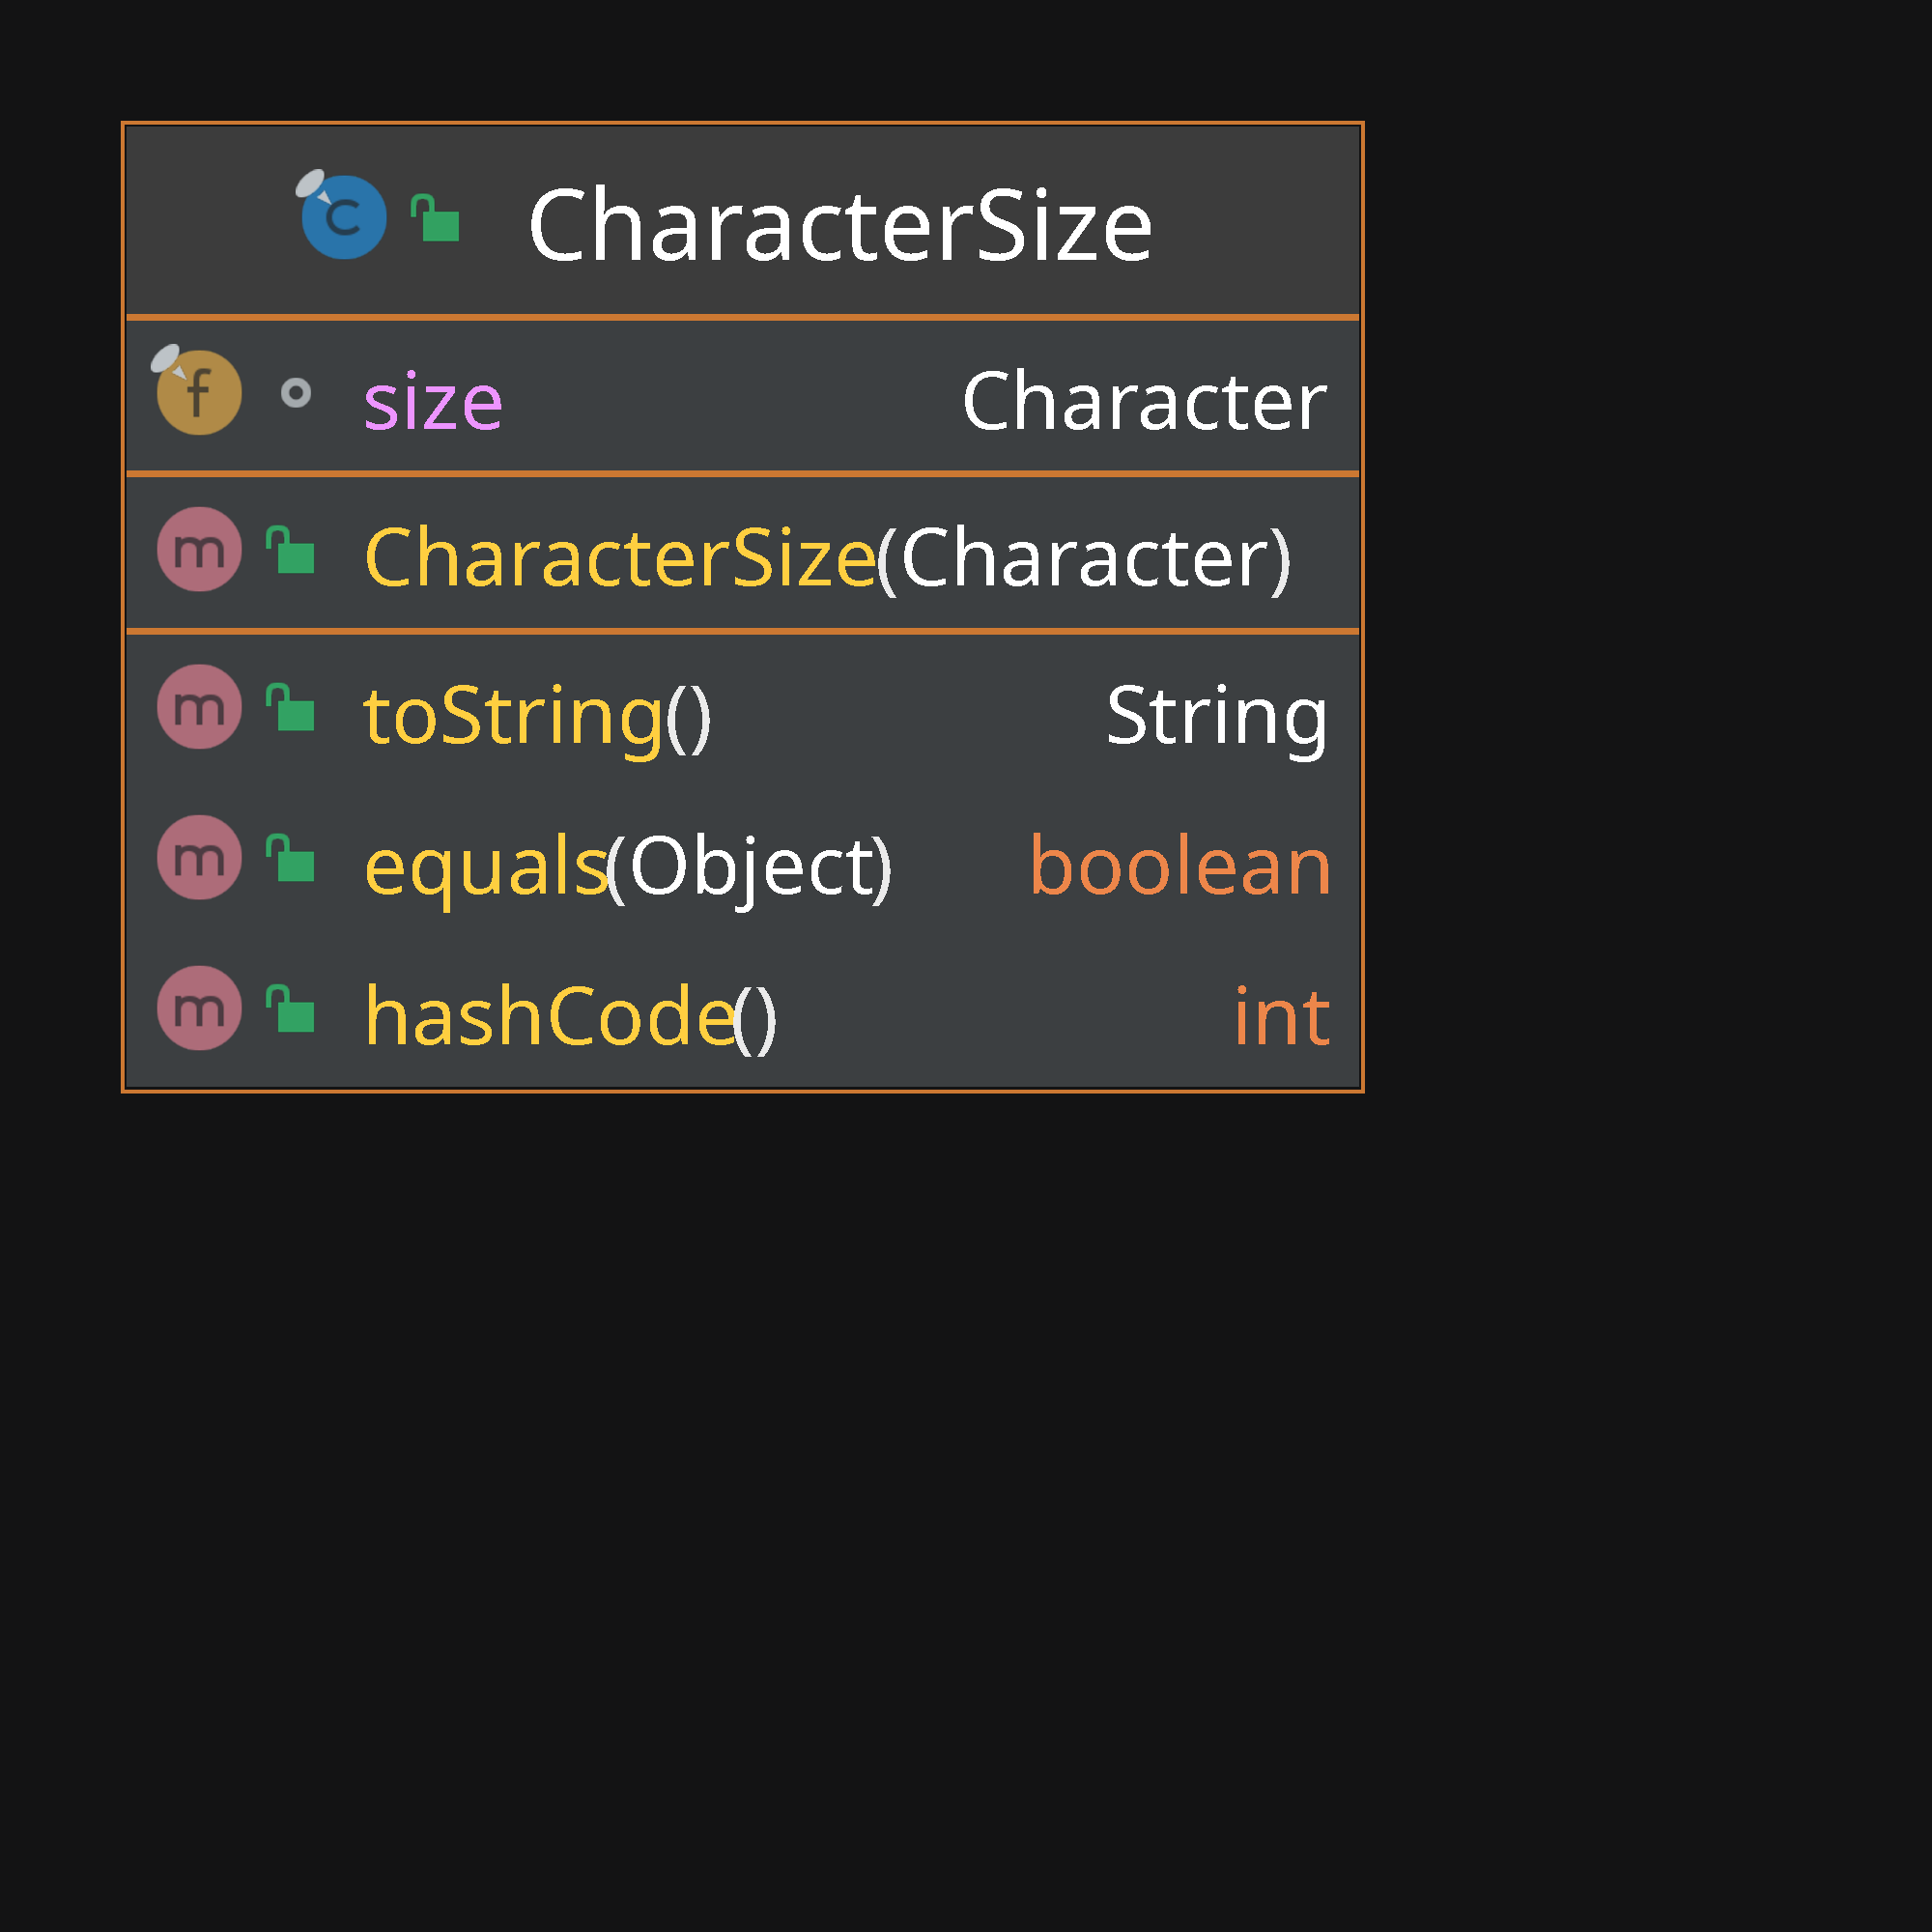
\includegraphics[width=0.4\textwidth]{Bilder/CharacterSize.pdf}
	\caption{UML der CharacterSize Klasse}
	\label{fig:Size}
\end{figure}
In der CharacterSize Klasse ist die Kohäsion hoch, da sie alle Funktionalitäten abdeckt, die die Größe des Charakters betreffen. Somit muss eine Änderung hier ausschließlich in dieser Klasse vorgenommen werden und nirgendwo anders.
\section{Don't Repeat Yourself (DRY)}
Gibt keinen. Ich habe von vornherein versucht duplizierten Code zu vermeiden.
\chapter{Unit Tests}
\section{10 Unit Tests}
Tabelle irgendwo in diesem Kapitel. Latex packt die dahin wo es das für richtig hält
\afterpage{%
	\clearpage% Flush earlier floats (otherwise order might not be correct)
	\thispagestyle{empty}% empty page style (?)
	\begin{landscape}% Landscape page
		\centering % Center table
		\begin{adjustbox}{center,caption={Evaluation der Datensätze},float=table,label={tab:Datasets}}
			\centering
			\label{tab:Datasets}
			\small
			\setlength{\tabcolsep}{3pt}
	\begin{tabular}{l|l}
		Unit Test                                & Beschreibung                                                                       \\ \hline
		RPGCharacterTest\#getAC()                & Es wird geprüft ob die Armor Class (AC) des Charackters korrekt berechnet wird.    \\ \hline
		RPGCharacterTest\#getSavingThrows()      & Es wird geprüft ob die SavingThrows Boni des Charackters korrekt berechnet werden. \\ \hline
		RPGCharacterTest\#getSkills()            & Es wird geprüft ob die Skill Boni des Charackters korrekt berechnet werden.        \\ \hline
		DeathSavesTest\#getFailures()            & Prüft ob die Anzahl an Fehlschlägen korrekt berechnet wird.                        \\ \hline
		DeathSavesTest\#getSuccesses()           & Prüft ob die Anzahl an Erfolgreichen Death Saves korrekt berechnet wird            \\ \hline
		DiceRollServiceTest\#rollInitiative()    & Prüft ob das Ergebnis des Initiative Wurfs korrekt berechnet wird                  \\ \hline
		DiceRollServiceTest\#attack()            & Prüft ob der Damage beim Ausführen einer Attacke korrekt berechnet wird            \\ \hline
		DiceRollServiceTest\#rollSkill()         & Prüft ob das Ergebnis eines Skill Rolls korrekt berechnet wird                     \\ \hline
		DiceRollServicetest\#rollSavingThrow()   & Prüft ob das Ergebnis eines SavingThrows korrekt berechnet wird                    \\ \hline
		CharacterServiceTest\#displayCharacter() & Prüft ob der String eines Charackters korrekt zusammengebaut wird.                
	\end{tabular}
       % \caption{Evaluation der Datensätze}
\end{adjustbox}
% Add 'table' caption
\end{landscape}
\clearpage% Flush page
}
\section{ATRIP: Automatic}
Automatic wurde auf zwei verschiedene Arten und weisen realisiert, einmal wurde die pom.xml des Maven Projektes im Hauptmodul der Applikation so angepasst, das das automatische Ausführen aller Tests Teil des Maven Workflows ist. Somit werden Tests automatisch mit jedem maven package, test und install ausgeführt. Sollte ein Test fehlschlagen, wird der jeweilige maven Workflow nicht erfolgreich abgeschlossen. Desweiteren wurde ein Github workflow zur automatischen Validierung aller Pullrequests und Commits angelegt. Dieser Workflow führt nach jedem Commit in einer isolierten Umgebung den maven package workflow aus. Kommt es während dieses zu einem Test Failure, schlägt der Workflow fehl und die Pullrequest kann nicht gemerged werden, oder es wird explizit am Commit ausgewiesen, dass dieser Commit fehlerhaft ist.

\clearpage
\section{ATRIP: Thorough}
\lstinputlisting[
label={code:diceRollThorough},  % Label; genutzt für Referenzen auf dieses Code-Beispiel
caption={Test der Attack Methode des DiceRollService},
captionpos=b,               % Position, für die Caption:  t(op) oder b(ottom)
language=java,     % Eigener Style der vor dem Dokument festgelegt wurde
firstline=36,                % Zeilennummer im Dokument welche als erste angezeigt wird
lastline=51,                 % Letzte Zeile welche ins LaTeX Dokument übernommen wird
basicstyle=\tiny
]{Quellcode/DiceRollServiceTest.java}
In Listing \ref{code:diceRollThorough}, ist ein Beispiel zu sehen, bei dem alle notwendigen Funktionalitäten der \texttt{attack()} Methode getestet werden. So testet der Unit Test das korrekte berechnen von Werten unter Einbezug aller möglicher Eigenschaften einer Waffe, sowie das auftreten von Exception, in dem absichtlich falsche Eingaben an die Funktion gereicht werden. Somit dekt dieser Test alle Funktionalitäten der Methode vollständig ab und hält damit das Thorough Prinzip ein. Im Vergleich dazu,hält der in Listing \ref{code:diceRollNotThorough} gezeigte Test dieses Prinzip nicht ein. Er überprüft nur eine mögliche valide Eingabe und prüft keine Randfälle und falsch Eingaben. Somit wird nicht kontrolliert, ob nach veränderungen Exceptions noch korrekt geworfen werden oder ob ungewollte Seiteneffekte auftreten. 
\lstinputlisting[
label={code:diceRollNotThorough},  % Label; genutzt für Referenzen auf dieses Code-Beispiel
caption={Test der rollSkill Methode des DiceRollService},
captionpos=b,               % Position, für die Caption:  t(op) oder b(ottom)
language=java,     % Eigener Style der vor dem Dokument festgelegt wurde
firstline=53,                % Zeilennummer im Dokument welche als erste angezeigt wird
lastline=56,                 % Letzte Zeile welche ins LaTeX Dokument übernommen wird
basicstyle=\tiny
]{Quellcode/DiceRollServiceTest.java}

\section{ATRIP: Professional}
\lstinputlisting[
label={code:diceRollProfessional},  % Label; genutzt für Referenzen auf dieses Code-Beispiel
caption={Auszug aus dem Test des DiceRollService, ganzes File: \href{https://github.com/lkno0705/DnD-CharacterManager/blob/main/2-dnd-charactermanager-application/src/test/java/rolls/DiceRollServiceTest.java}{https://github.com/lkno0705/DnD-CharacterManager/blob/main/2-dnd-charactermanager-application/src/test/java/rolls/DiceRollServiceTest.java}},
captionpos=b,               % Position, für die Caption:  t(op) oder b(ottom)
language=java,     % Eigener Style der vor dem Dokument festgelegt wurde
firstline=63,                % Zeilennummer im Dokument welche als erste angezeigt wird
lastline=97,                 % Letzte Zeile welche ins LaTeX Dokument übernommen wird
basicstyle=\tiny
]{Quellcode/DiceRollServiceTest.java}
Listing \ref{code:diceRollProfessional} zeigt ein positives Beispiel des Professional Prinzips. In diesem Beispiel wurde Test Code wie Produktivcode behandelt und es wurde darauf geachtet, den Prozess des Mockings anstatt in einer riesigen Methode in mehrere kleine Untermethoden zu unterteilen. Somit ist der Code gut wartbar und falls eine Änderung gemacht werden muss, kann man sofort zu der jeweiligen Methode springen und muss nicht in einer Wall of Text die entsprechende Stelle raussuchen. Des weiteren kümmert sich jede Methode in diesem Beispiel genau um eine einzige Funktionalität. Somit wird in jeder Methode nur genau ein Mockobjekt generiert.
\lstinputlisting[
label={code:diceRollNotProfessional},  % Label; genutzt für Referenzen auf dieses Code-Beispiel
caption={Auszug aus dem Test des DiceRollService, ganzes File: \href{https://github.com/lkno0705/DnD-CharacterManager/blob/main/2-dnd-charactermanager-application/src/test/java/character/CharacterServiceTest.java}{https://github.com/lkno0705/DnD-CharacterManager/blob/main/2-dnd-charactermanager-application/src/test/java/character/CharacterServiceTest.java}},
captionpos=b,               % Position, für die Caption:  t(op) oder b(ottom)
language=java,     % Eigener Style der vor dem Dokument festgelegt wurde
firstline=118,                % Zeilennummer im Dokument welche als erste angezeigt wird
lastline=136,                 % Letzte Zeile welche ins LaTeX Dokument übernommen wird
basicstyle=\tiny
]{Quellcode/CharacterServiceTest.java}
Wie in Listing \ref{code:diceRollNotProfessional} kommt das Mocking von \texttt{HitDice}, \texttt{Weapons} etc. in anderen Tests auch zum Einsatz. Trotz dessen das auch in diesen Tests darauf geachtet wurde, den Mocking Prozess in kleine Methoden aufzuspalten und somit die Wartbarkeit und lesbarkeit zu erhöhen, stellt dies doch auch gleichzeitig ein negativ Beispiel dar. Da nun in jedem Test der ein Entsprechendes Objekt mockt, eine Änderung gemacht werden muss, wenn etwas an den jeweiligen Domain Objekten geändert wurde. Somit währe es hier sinnvoll gewesen, den Mocking Prozess in eine Utility Class auszulagern. Dies würde nicht nur die Wartbarkeit und lesbarkeit des Tests verbessern, sondern auch gleichzeitig die komplexität der Tests verringern.

\section{Code Coverage}
\begin{figure}[H]
	\centering
	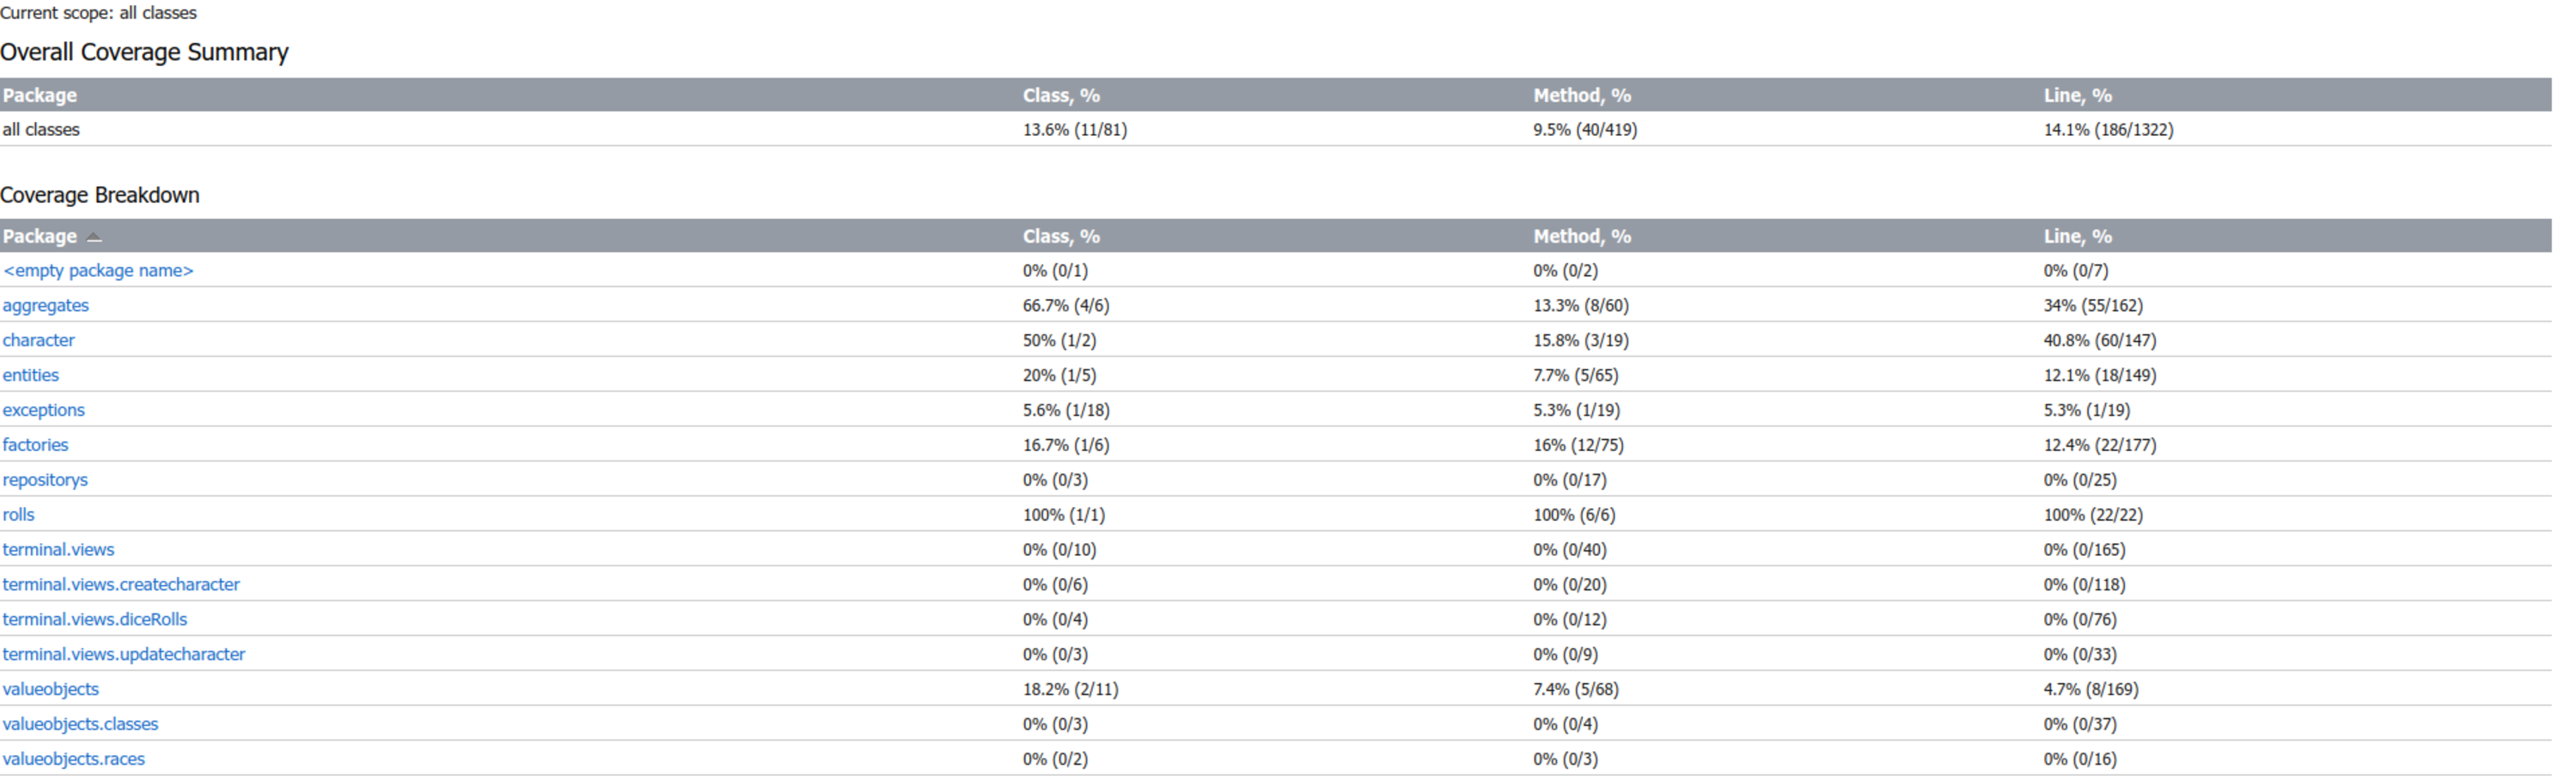
\includegraphics[width=\textwidth]{Bilder/CodeCoverage.pdf}
	\caption{Code Coverage Report generiert von IntelliJ}
	\label{fig:CodeCoverage}
\end{figure}
Abbildung \ref{fig:CodeCoverage} zeigt den Code Coverage report der Tests über das gesamte Projekt. Die generelle Coverage ist mit einer Line Coverage von 14.1\%, einer Class Coverage von 13.6\% und einer Method Coverage von 9.5\% recht gering. Dies liegt daran das der größte Teil des Projektes ausschließlich aus der Modellierung von Domänenobjekten besteht, die ausschließlich Setter und Getter enthalten und nicht sehr viel Logik mit sich bringen. Diese Objekte werden in den jeweiligen Unit Tests durch mocks ersetzt und somit nicht durchlaufen. Daher entstehen sehr geringe Coverage Prozent zahlen. In Packages wie dem \texttt{rolls} Package ist das anders. Dieses Package enthält die UseCases des \texttt{DiceRollService}, die jeweils für den Nutzer wichtige Ergebnisse berechnen. Diese lassen sich sinnvoll und gut testen. Somit erreicht die Code Coverage in diesem Package auch einen Wert von 100\% in allen 3 Coverage Kategorien. Um die Code Coverage zu verbessern wären in diesem Projekt Integration Tests sinnvoll. Da sie neben der reinen Funktionalität einzelner Methoden, auch das zusammenspiel der einzelnen Klassen und Objekte prüfen und somit auch prüfen können ob Dinge richtig gesetzt und gelesen werden und ob die Semantik der Prozesse korrekt ist.

\section{Fakes und Mocks}
\begin{figure}[H]
	\centering
	\includegraphics[width=\textwidth]{Bilder/CharacterServiceTest.pdf}
	\caption{Abhängigkeiten der CharacterService Klasse}
	\label{fig:Mocks}
\end{figure}
Wie Abbildung \ref{fig:Mocks} zu entnehmen ist, hängt die Klasse \texttt{CharacterService} von allen Klassen der Domain Schicht ab und hat somit sehr viele Abhängigkeiten. Ein Unit Test soll jedoch möglichst wenige bis gar keine Abhängigkeiten besitzen, um den Test und die auftretenden Effekte auf einen Ort zu isolieren und zu beschränken. Um dies zu ermöglichen und die Abhängigkeiten der Klassen zu reduzieren, wurde jedes einzelne Objekt, von dem der \texttt{CharacterService} abhängig ist durch einen Mock / einen Fake ersetzt. Dementsprechend wurden folgende Klassen ersetzt:
\begin{itemize}
	\item \texttt{HitDie}
	\item \texttt{Weapon}
	\item \texttt{RepositoryService}
	\item \texttt{Player}
	\item \texttt{CharacterClass}
	\item \texttt{Personality}
	\item \texttt{Background}
	\item \texttt{CharacterRace}
	\item \texttt{DeathSaves}
	\item \texttt{Attributes}
	\item \texttt{Currencys}
	\item \texttt{Armor}
	\item \texttt{Inventory}
	\item \texttt{RPGCharacter}
\end{itemize}
Wären diese Objekte nicht durch Fakes ersetzt worden, hätte dieser Test praktisch das gesamte Projekt getestet. Ein ähnlicher Fall stellt auch der \texttt{DiceRollServiceTest} dar, auch wenn dieser weniger Abhängigkeiten besitzt.
\chapter{Domain Driven Design}
\section{Ubiquitous Language}
[4 Beispiele für die Ubiquitous Language; jeweils Bezeichung, Bedeutung und kurze Begründung, warum es zur Ubiquitous Language gehört]
\begin{table}[!ht]
\centering
\begin{tabular}{lll}
\textbf{Bezeichnung} & \textbf{Bedeutung} & \textbf{Begründung} \\
Klasse               & tbw                & tbw                 \\
Rasse                & tbw                & tbw                 \\
Equipment            & tbw                & tbw                 \\
Spell                & tbw                & tbw                
\end{tabular}
\end{table}

\FloatBarrier
\section{Entities}
[UML, Beschreibung und Begründung des Einsatzes einer Entity; falls keine Entity vorhanden: ausführliche Begründung, warum es keines geben kann/hier nicht sinnvoll ist]

\section{Value Objects}
[UML, Beschreibung und Begründung des Einsatzes eines Value Objects; falls kein Value Object vorhanden: ausführliche Begründung, warum es keines geben kann/hier nicht sinnvoll ist]

\section{Repositories}
[UML, Beschreibung und Begründung des Einsatzes eines Repositories; falls kein Repository vorhanden: ausführliche Begründung, warum es keines geben kann/hier nicht sinnvoll ist]

\section{Aggregates}
[UML, Beschreibung und Begründung des Einsatzes eines Aggregates; falls kein Aggregate vorhanden: ausführliche Begründung, warum es keines geben kann/hier nicht sinnvoll ist]
\chapter{Refactoring}

\section{Code Smells}
\begin{lstlisting}[
	captionpos=b,
	caption={Beschreibung eines in einem Bild enthaltenen Objektes mittels des Yolo Datei Formats},
	label={code:LongParameterList},
	language=java,
	escapeinside={@}{@}]
	public RPGCharacter(CharacterRace race, CharacterClass characterClass, Background background, Inventory inventory, String name, Attributes attributes, DeathSaves deathSaves, Player player, int xp, int age) throws RPGCharacterException
\end{lstlisting}
Listing \ref{code:LongParameterList} zeigt den Konstruktor der Klasse \texttt{RPGCharakter}. Dieser stellt den CodeSmell Long Parameter List dar. Um diesen zu lösen, müsste man mehrere der bereits zusammengefassten Objekte in weitere Objekte zusammenfassen. So wäre es z.B. möglich die Parameter \texttt{race}, \texttt{characterClass}, \texttt{Background}, \texttt{Attributes} in ein neues Objekt namens \texttt{CharacterProperties} zusammen zu fassen.

Die gesamte Klasse \texttt{InventoryService} besteht aus dead code. Sie wurde im Vorfeld angelegt um Änderungen im Inventory vornehmen zu können. Später wurde der Scope des Projektes jedoch verändert und der Code wird nicht mehr benötigt, wurde aber nicht gelöscht. Dementsprächend wäre es sinnvoll diesen Code nun zu löschen.

\section{2 Refactorings}
\subsection{Rename Method}
\begin{figure}[H]
	\centering
	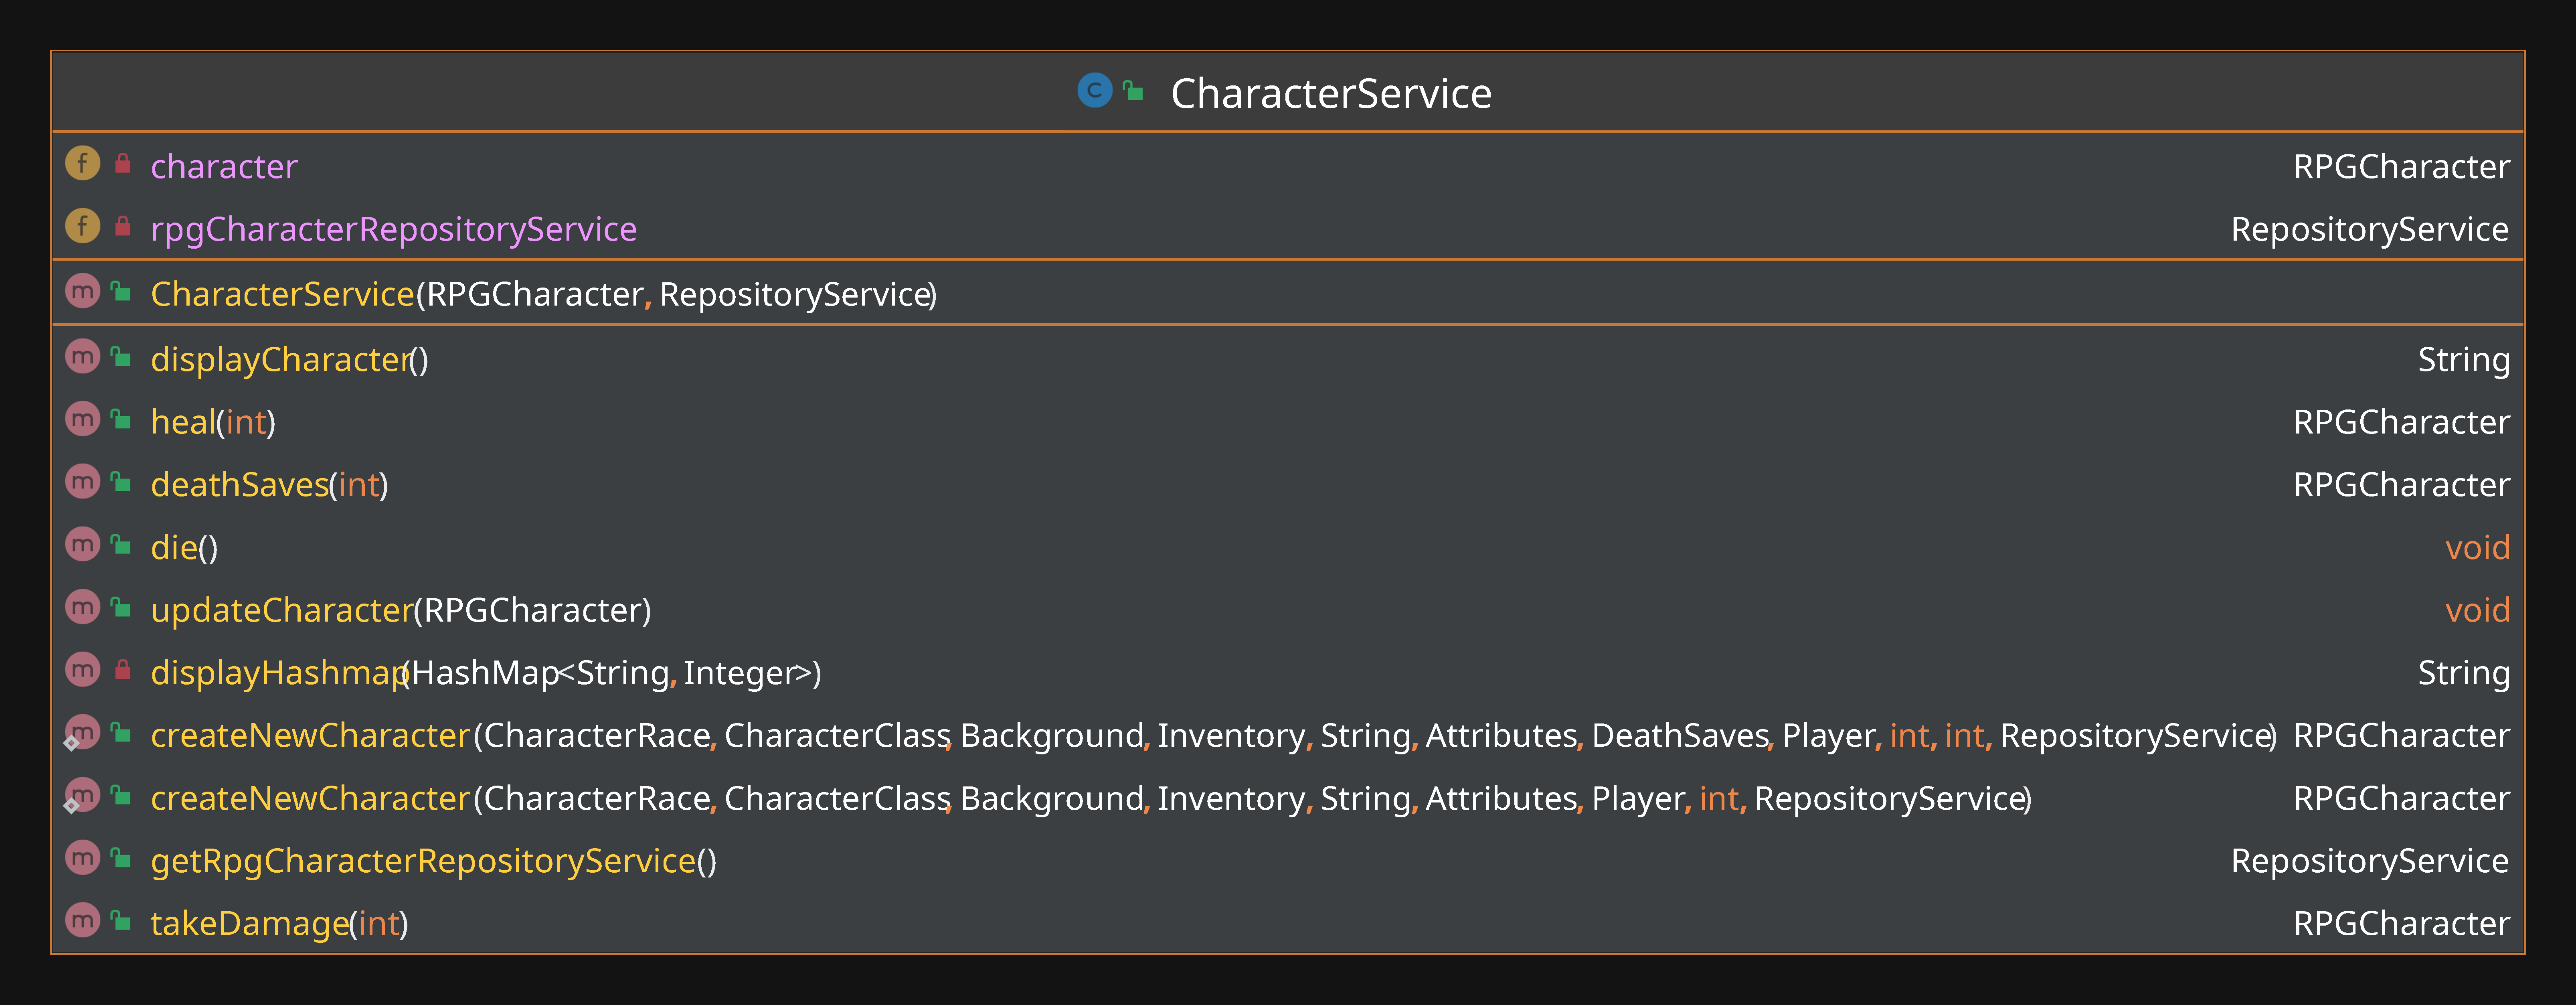
\includegraphics[width=0.49\textwidth]{Bilder/CharacterService-old.pdf}
	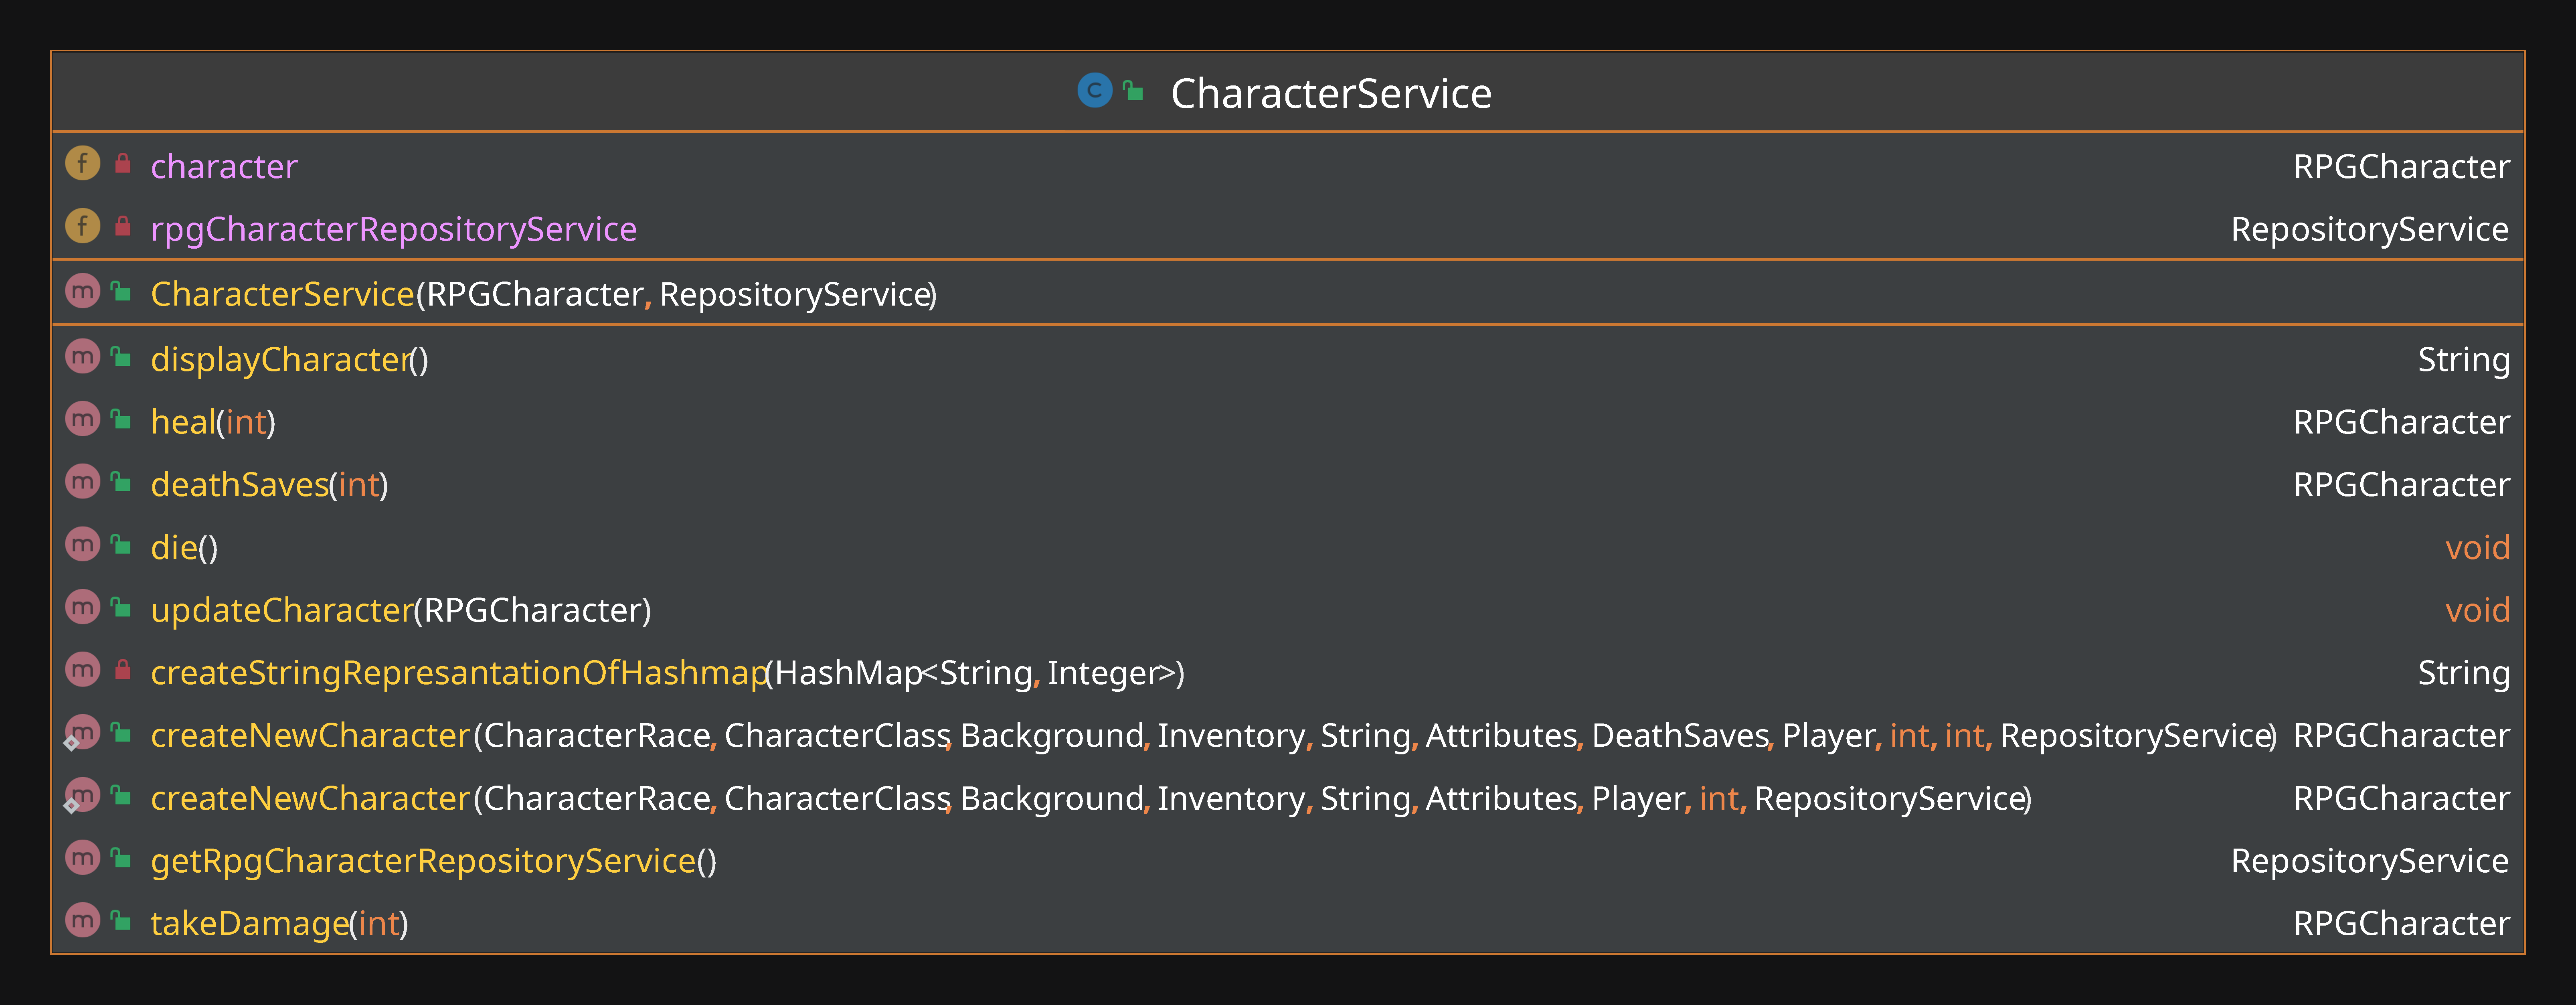
\includegraphics[width=0.49\textwidth]{Bilder/CharacterService.pdf}
	\caption{UML Diagramm des Character Service vor und nach dem Refactoring}
	\label{fig:rename}
\end{figure}
Die Methode \texttt{displayHashmap} wurde in \texttt{createStringRepresantationOfHashmap} umbennant, da die Methode keine Hashmap darstellt, sondern eine Stringrepräsentation einer übergebenen Hashmap baut und zurück gibt. Die UML Diagramme sind in Abbildung \ref{fig:rename} dargestellt. Alter commit: \href{https://github.com/lkno0705/DnD-CharacterManager/blob/497c202ebeea385178f9d1bca4aeb3401d92619c/2-dnd-charactermanager-application/src/main/java/character/CharacterService.java}{https://github.com/lkno0705/DnD-CharacterManager/blob/497c202ebeea385178f9d1bca4aeb3401d92619c/2-dnd-charactermanager-application/src/main/java/character/CharacterService.java}. Neuer commit: \href{https://github.com/lkno0705/DnD-CharacterManager/blob/main/2-dnd-charactermanager-application/src/main/java/character/CharacterService.java}{https://github.com/lkno0705/DnD-CharacterManager/blob/main/2-dnd-charactermanager-application/src/main/java/character/CharacterService.java}

\subsection{Extract Method}
\begin{figure}[H]
	\centering
	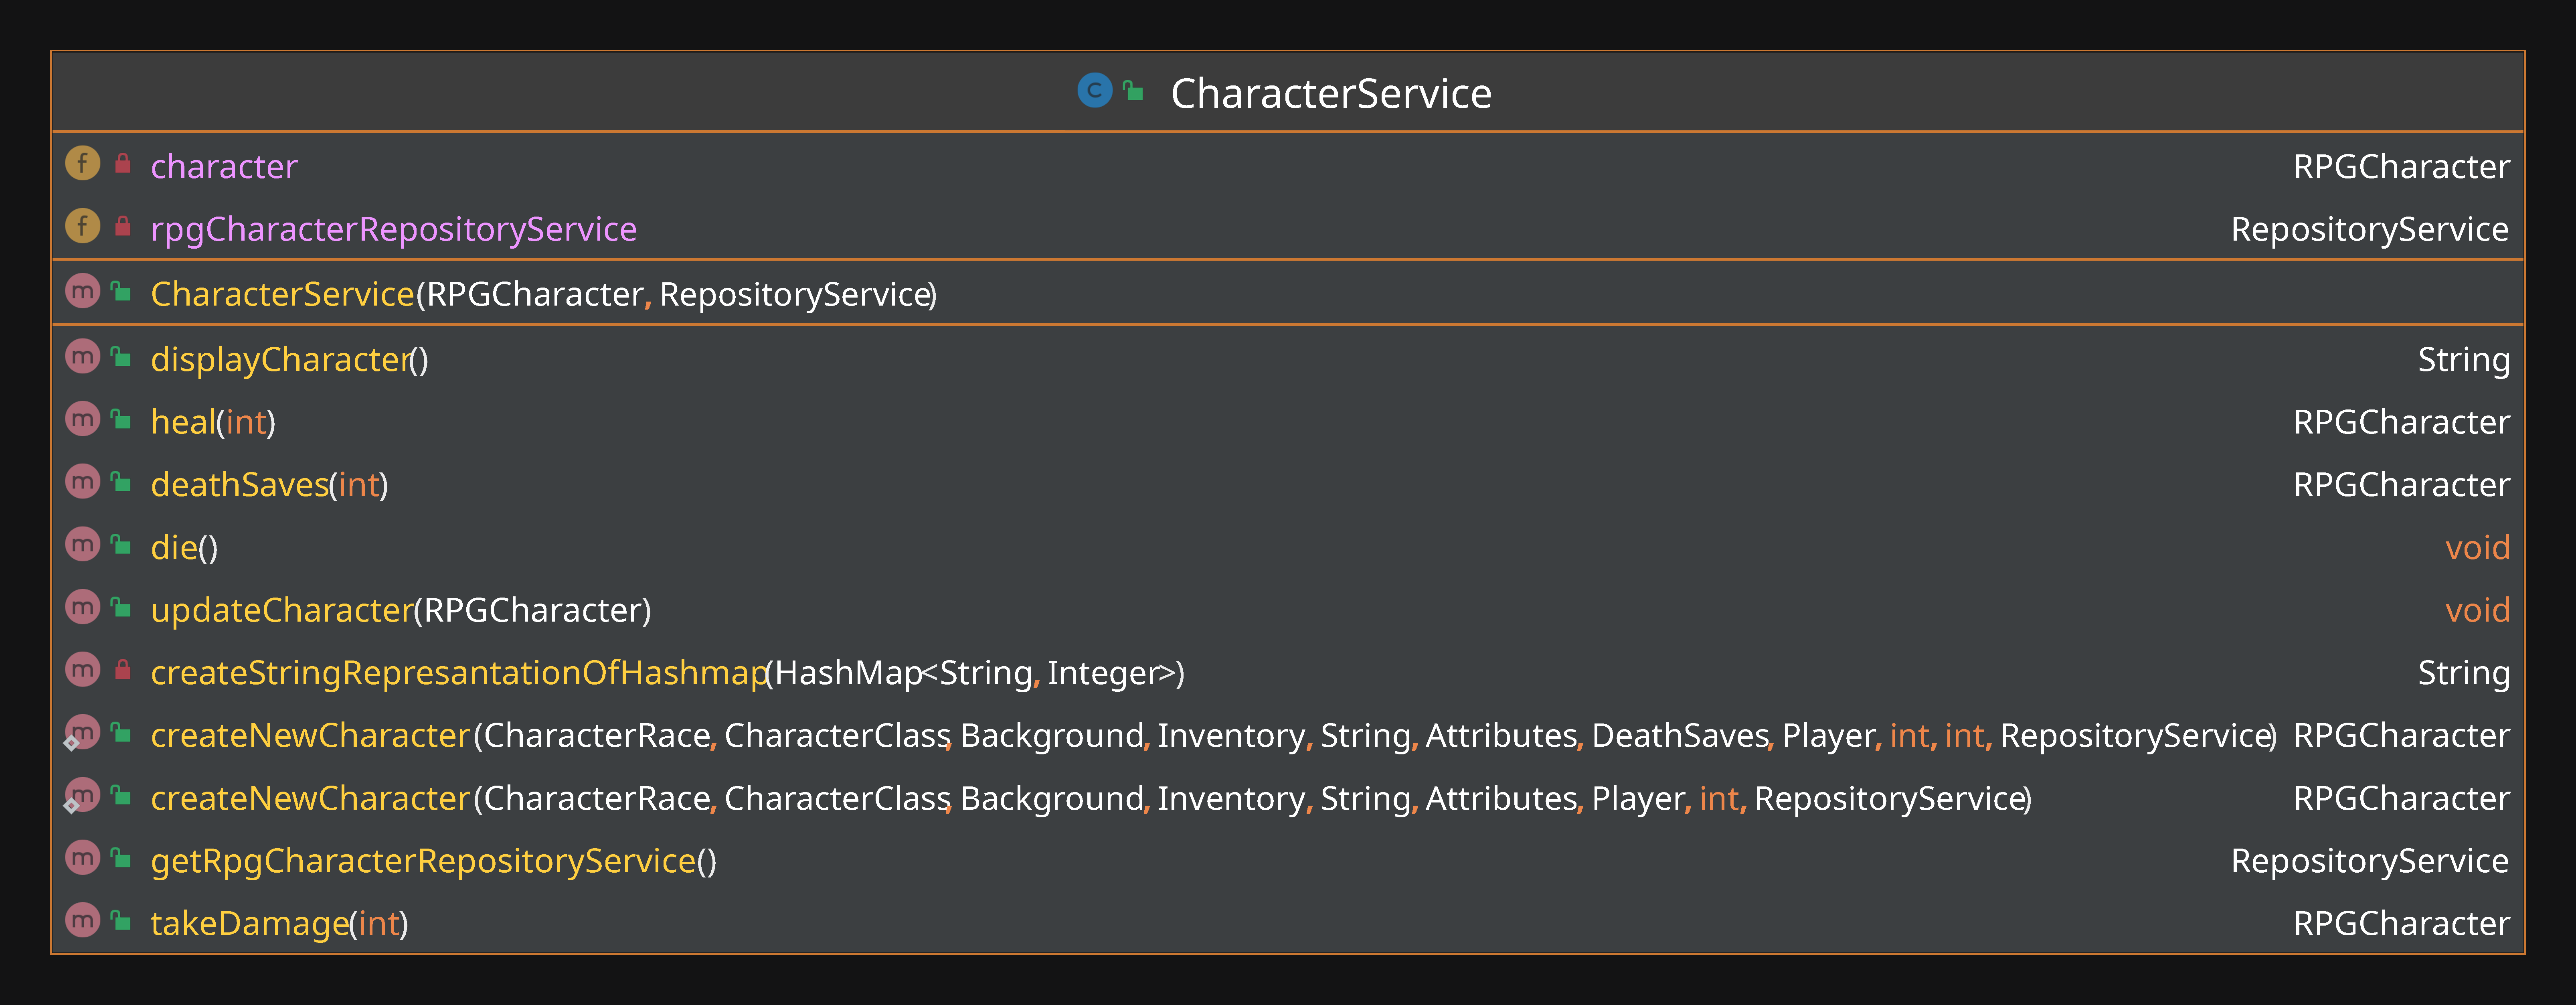
\includegraphics[width=0.49\textwidth]{Bilder/CharacterService.pdf}
	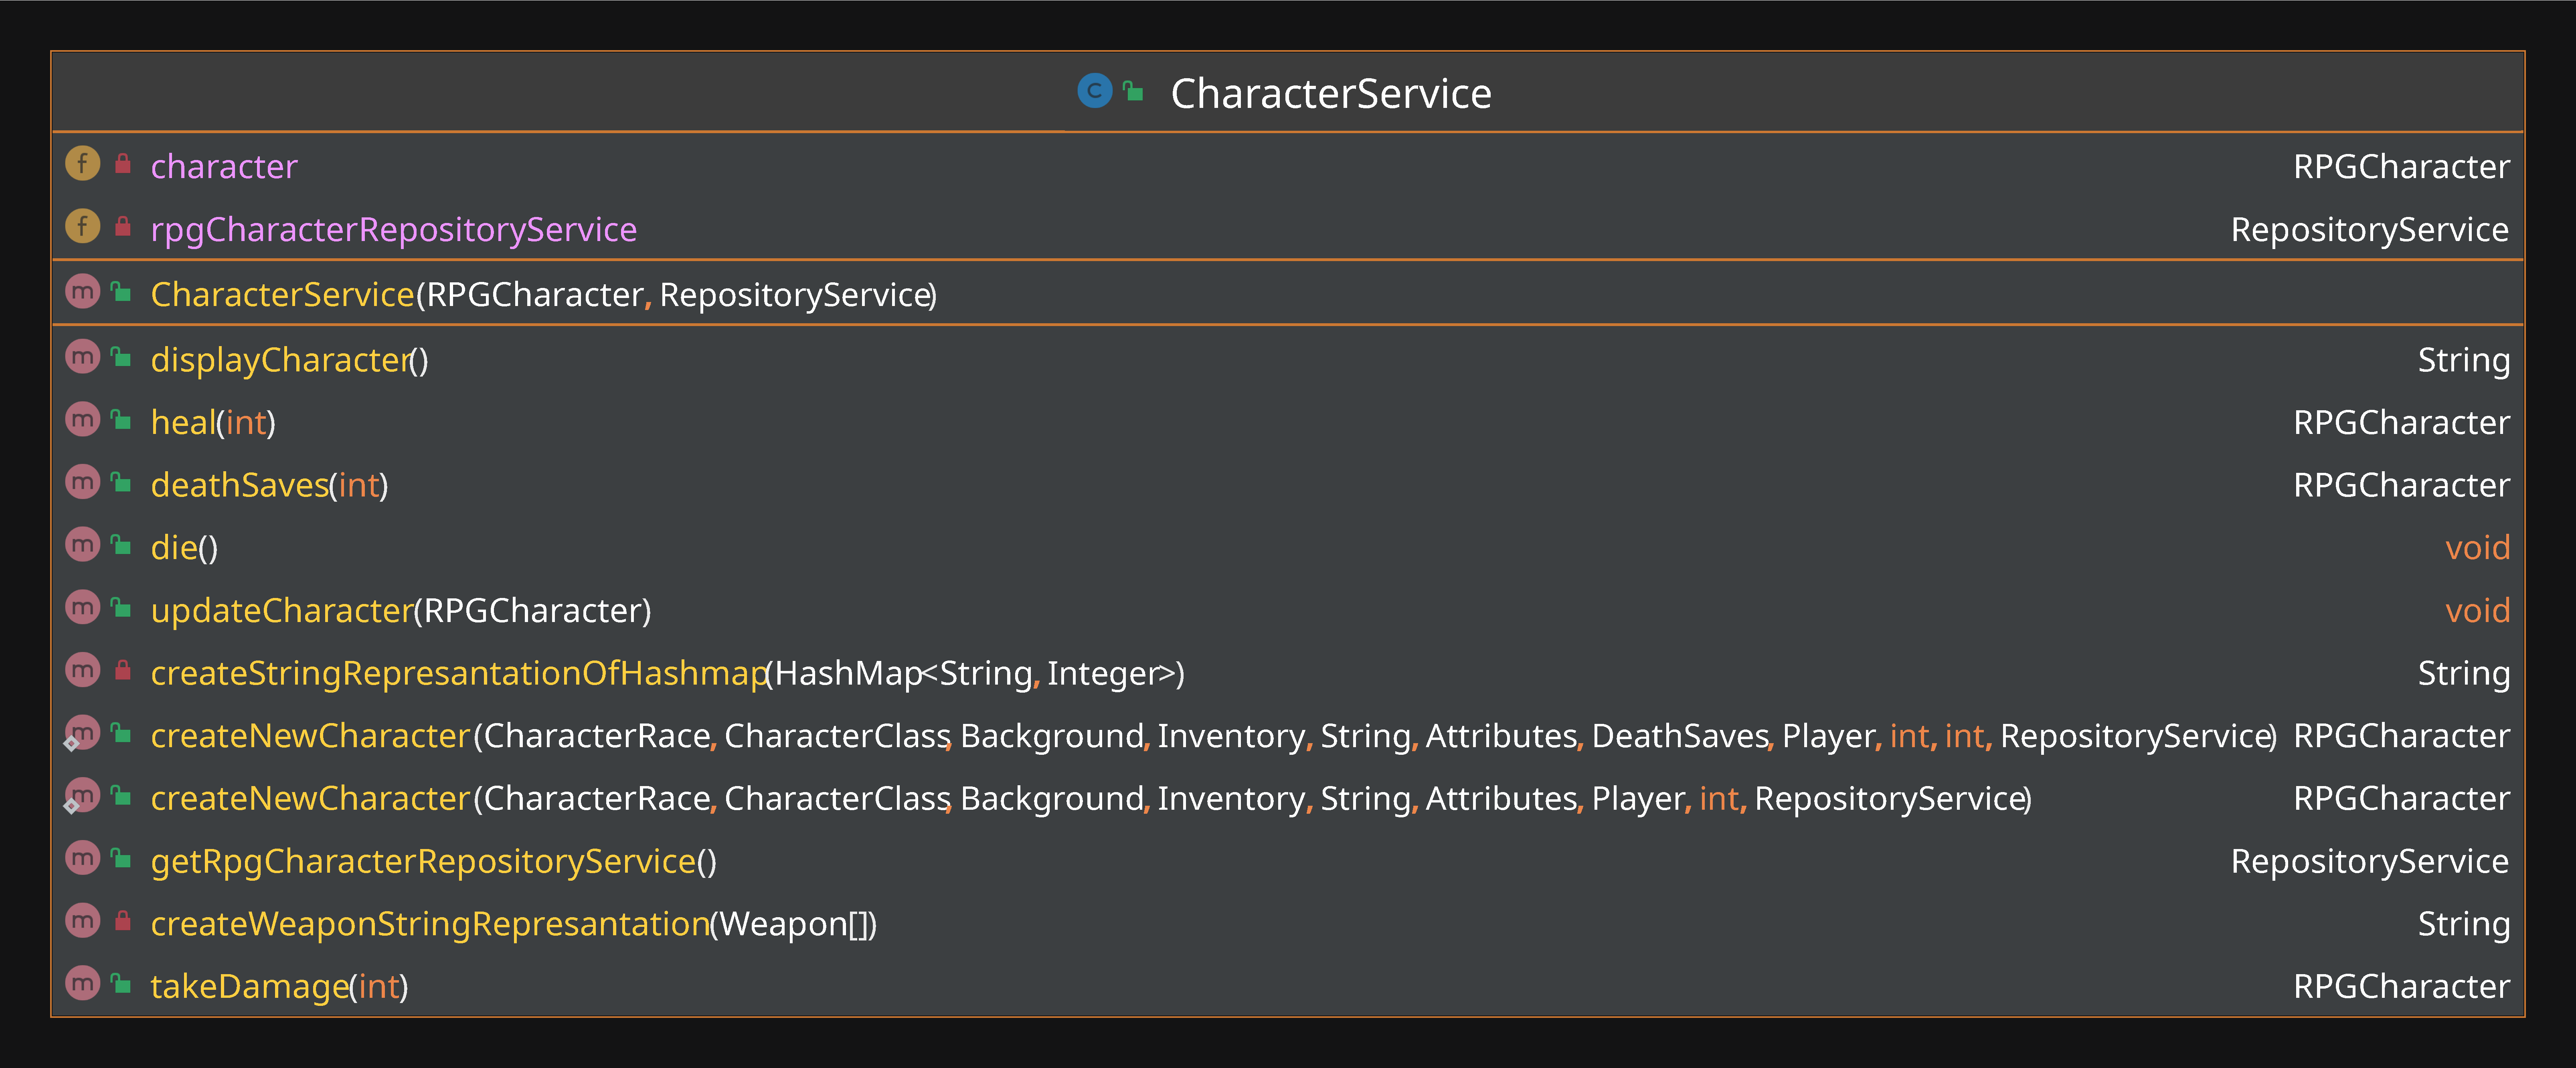
\includegraphics[width=0.49\textwidth]{Bilder/CharacterService-extracted.pdf}
	\caption{UML Diagramm des Character Service vor und nach dem Refactoring}
	\label{fig:extract}
\end{figure}
In der Methode \texttt{displayCharacter}, wurde eine \texttt{for-Schleife} extrahiert, die eine String Repräsentation des Waffen arrays des Inventorys aufgebaut hat. Dies dient dazu die recht lange Methode \texttt{displayCharacter} weiter zu verkürzen und so ihre lesbarkeit zu erhöhen.
Alter commit: \href{https://github.com/lkno0705/DnD-CharacterManager/blob/main/2-dnd-charactermanager-application/src/main/java/character/CharacterService.java}{https://github.com/lkno0705/DnD-CharacterManager/blob/main/2-dnd-charactermanager-application/src/main/java/character/CharacterService.java}. Neuer commit: \href{https://github.com/lkno0705/DnD-CharacterManager/blob/1469ce1aef5b10f2685ddd448b7028230aa0ba46/2-dnd-charactermanager-application/src/main/java/character/CharacterService.java}{https://github.com/lkno0705/DnD-CharacterManager/blob/1469ce1aef5b10f2685ddd448b7028230aa0ba46/2-dnd-charactermanager-application/src/main/java/character/CharacterService.java}

\chapter{Entwurfsmuster}

\section{Entwurfsmuster:  Erbauer}
\begin{figure}[H]
	\centering
	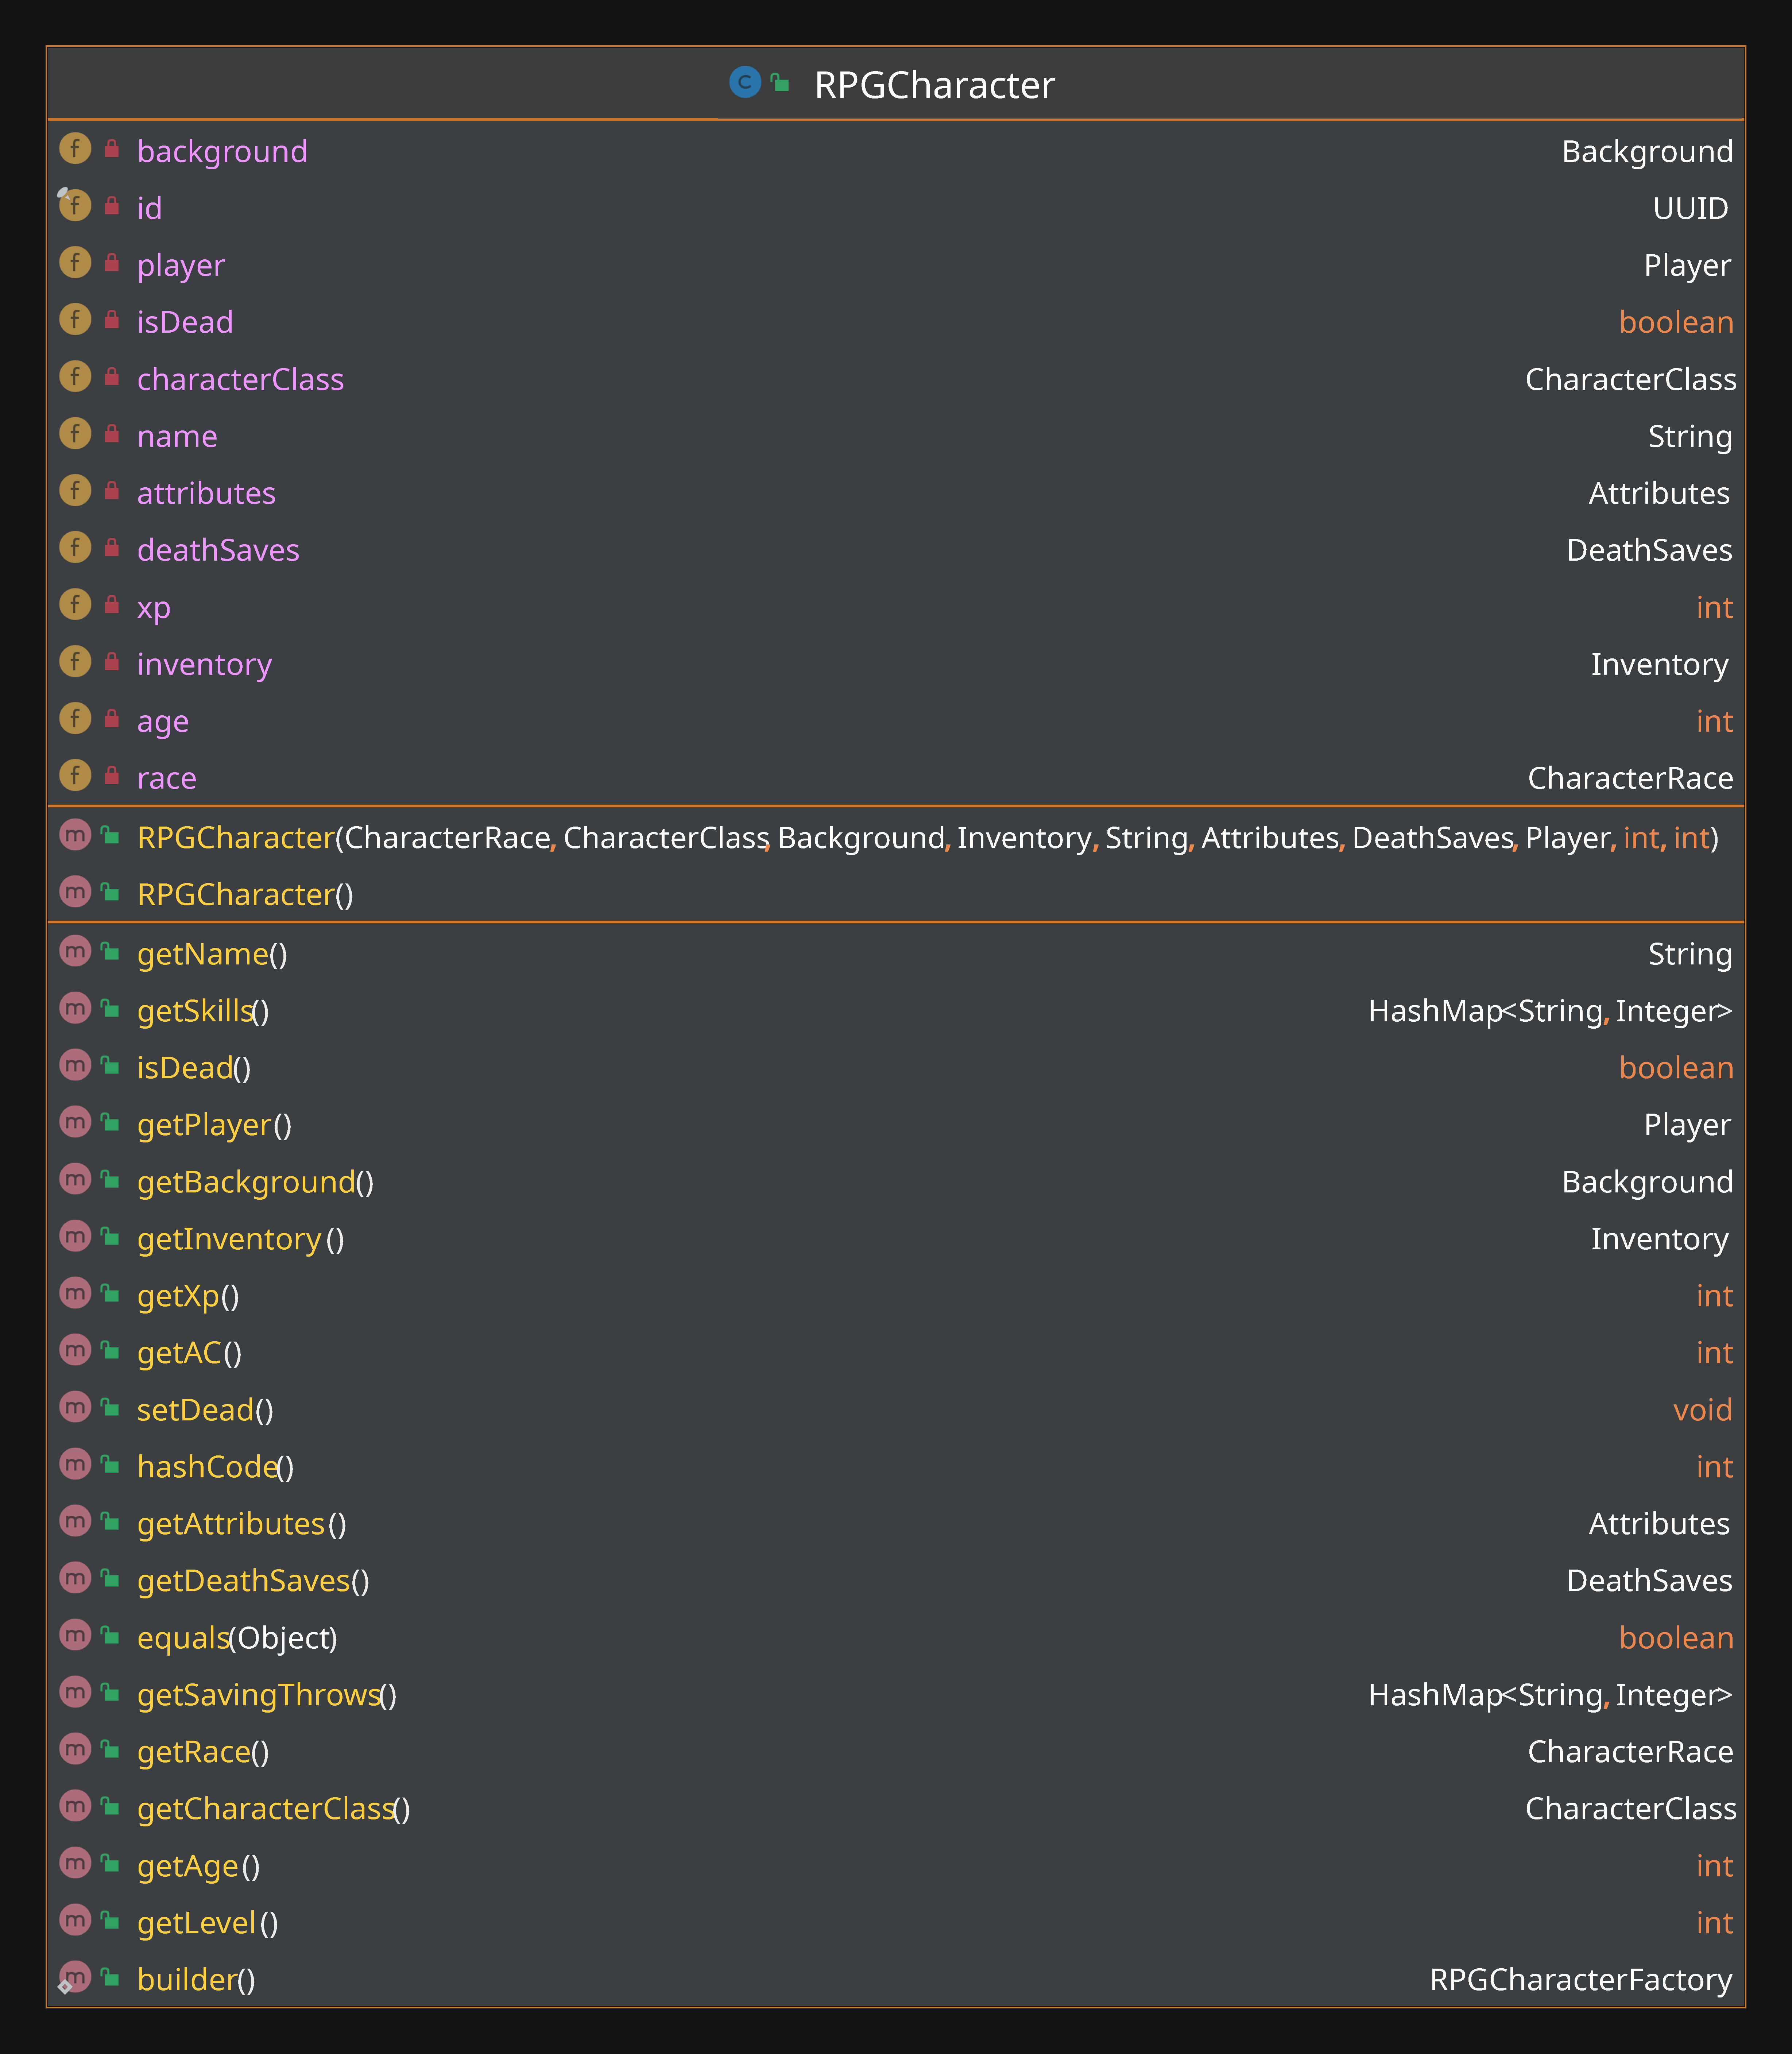
\includegraphics[width=0.4\textwidth]{Bilder/RPGCharacter.pdf}
		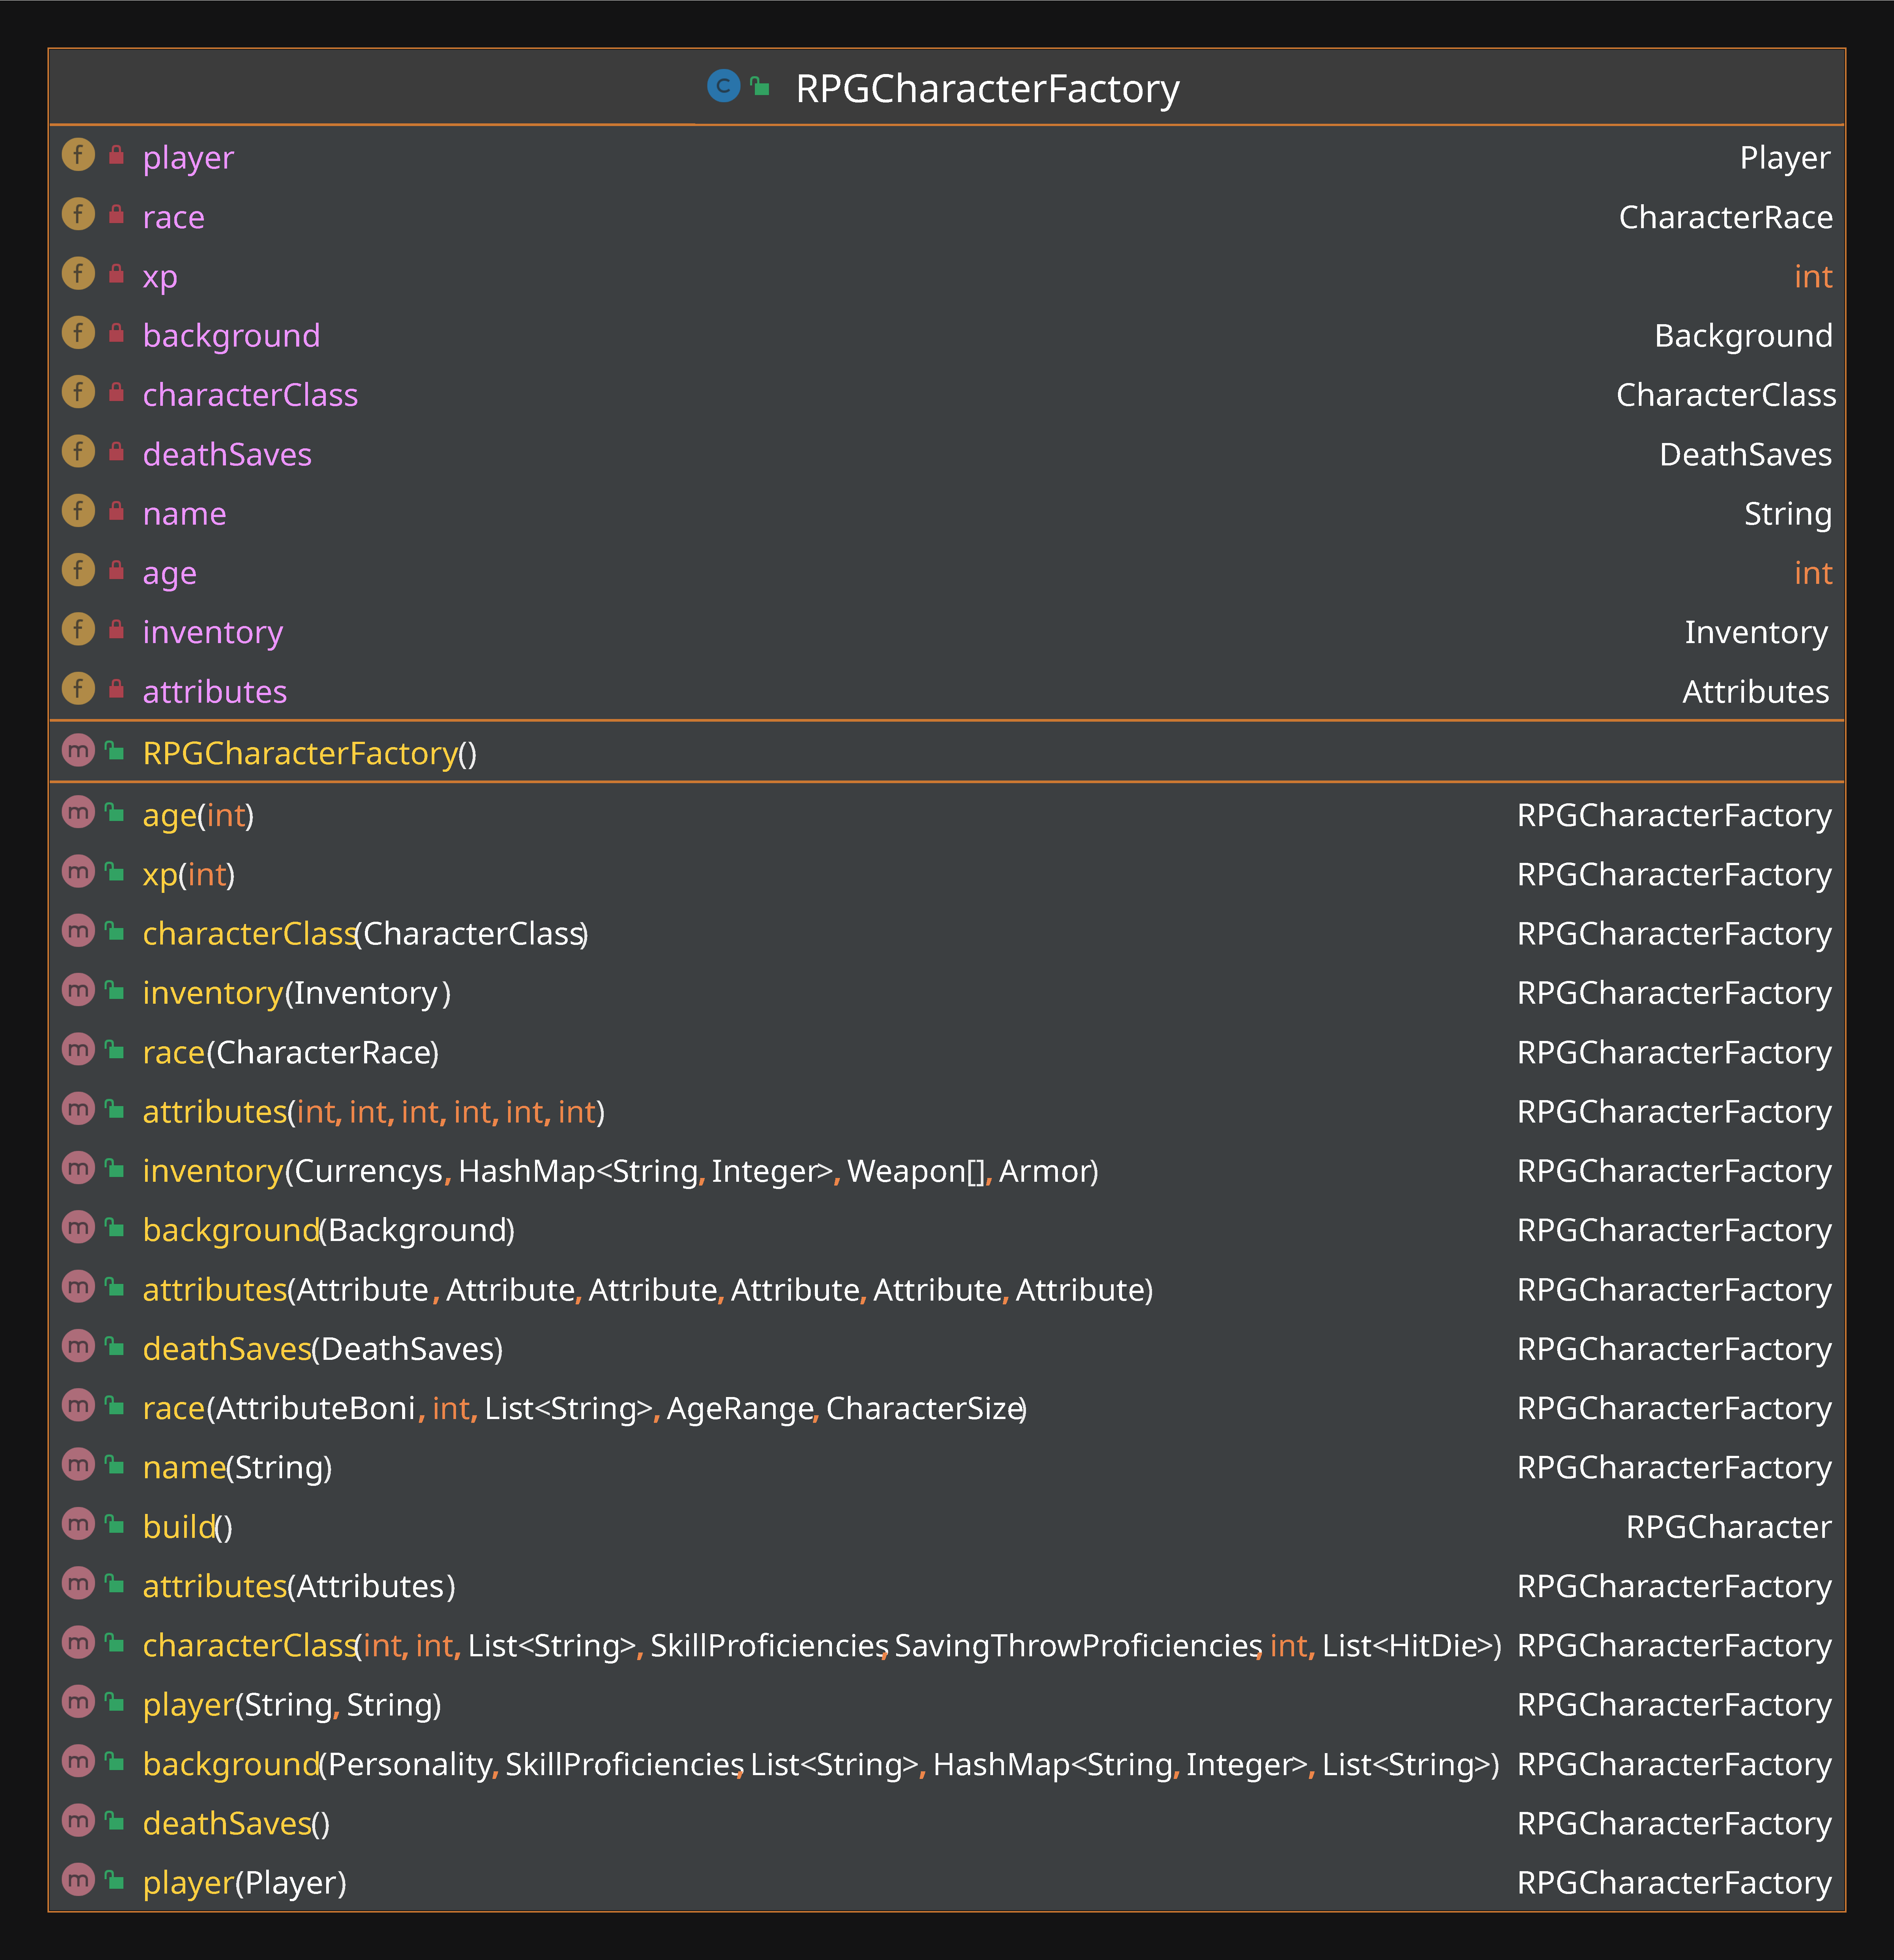
\includegraphics[width=0.4\textwidth]{Bilder/RPGCharacterFactory.pdf}
	\caption{UML der RPGChracter und der RPGCharacterFactory Klasse}
	\label{fig:factory}
\end{figure}
Um komplexe Objekte, wie z.B.: den \texttt{RPGCharacter} zu erzeugen, wurde das Erbauer Entwurfsmuster eingesetzt. Dieses ermöglicht es die Objekte Schritt für Schritt auf verschiedene Art und weisen zu Erzeugen und stellt gleichzeitig noch die Korrektheit der Objekte sicher. Abbildung \ref{fig:factory} zeigt die UML Diagramme der \texttt{RPGCharacter} Klasse und des dazugehörigen Erbauers. Dies verhindert das sehr lange Konstruktoren und Parameter auf einmal zur Objekterzeugung verwendet werden müssen und ermöglicht eine einfachere Handhabung der Objekterstellung in höheren Schichten.

\section{Entwurfsmuster:  Stellvertreterle}
\begin{figure}[H]
	\centering
	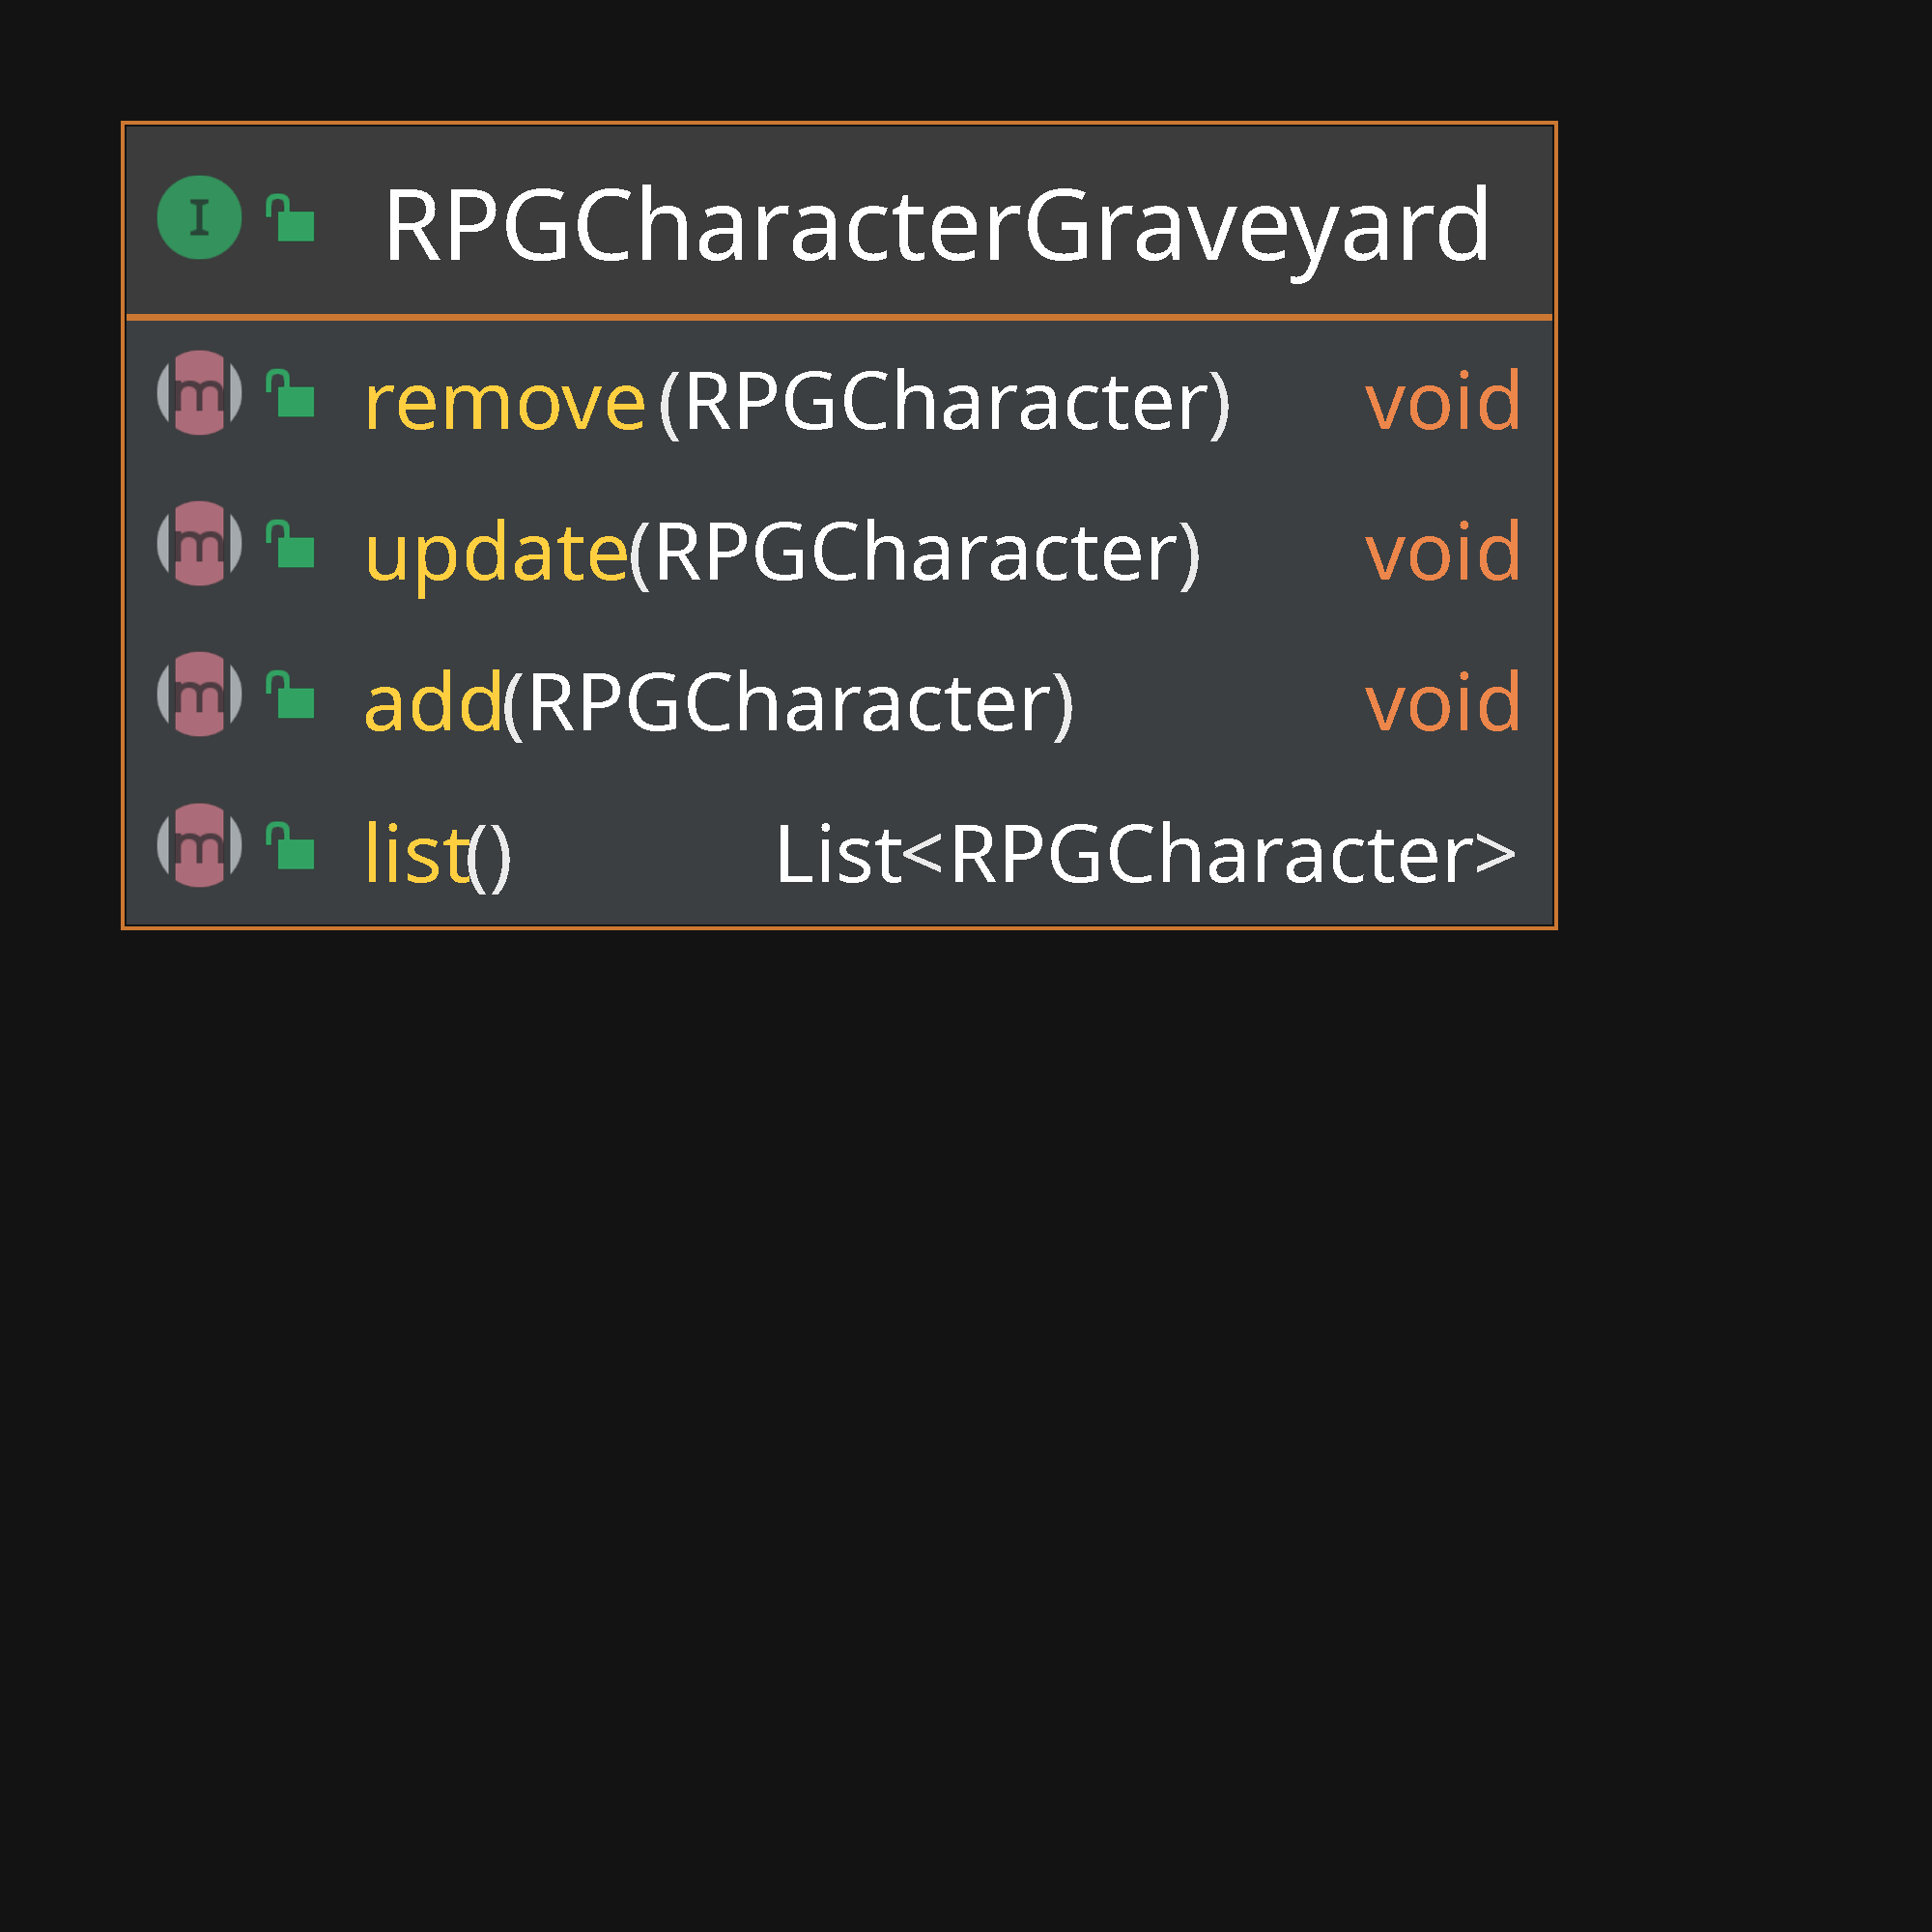
\includegraphics[width=0.4\textwidth]{Bilder/RPGCharacterGraveyard.pdf}
	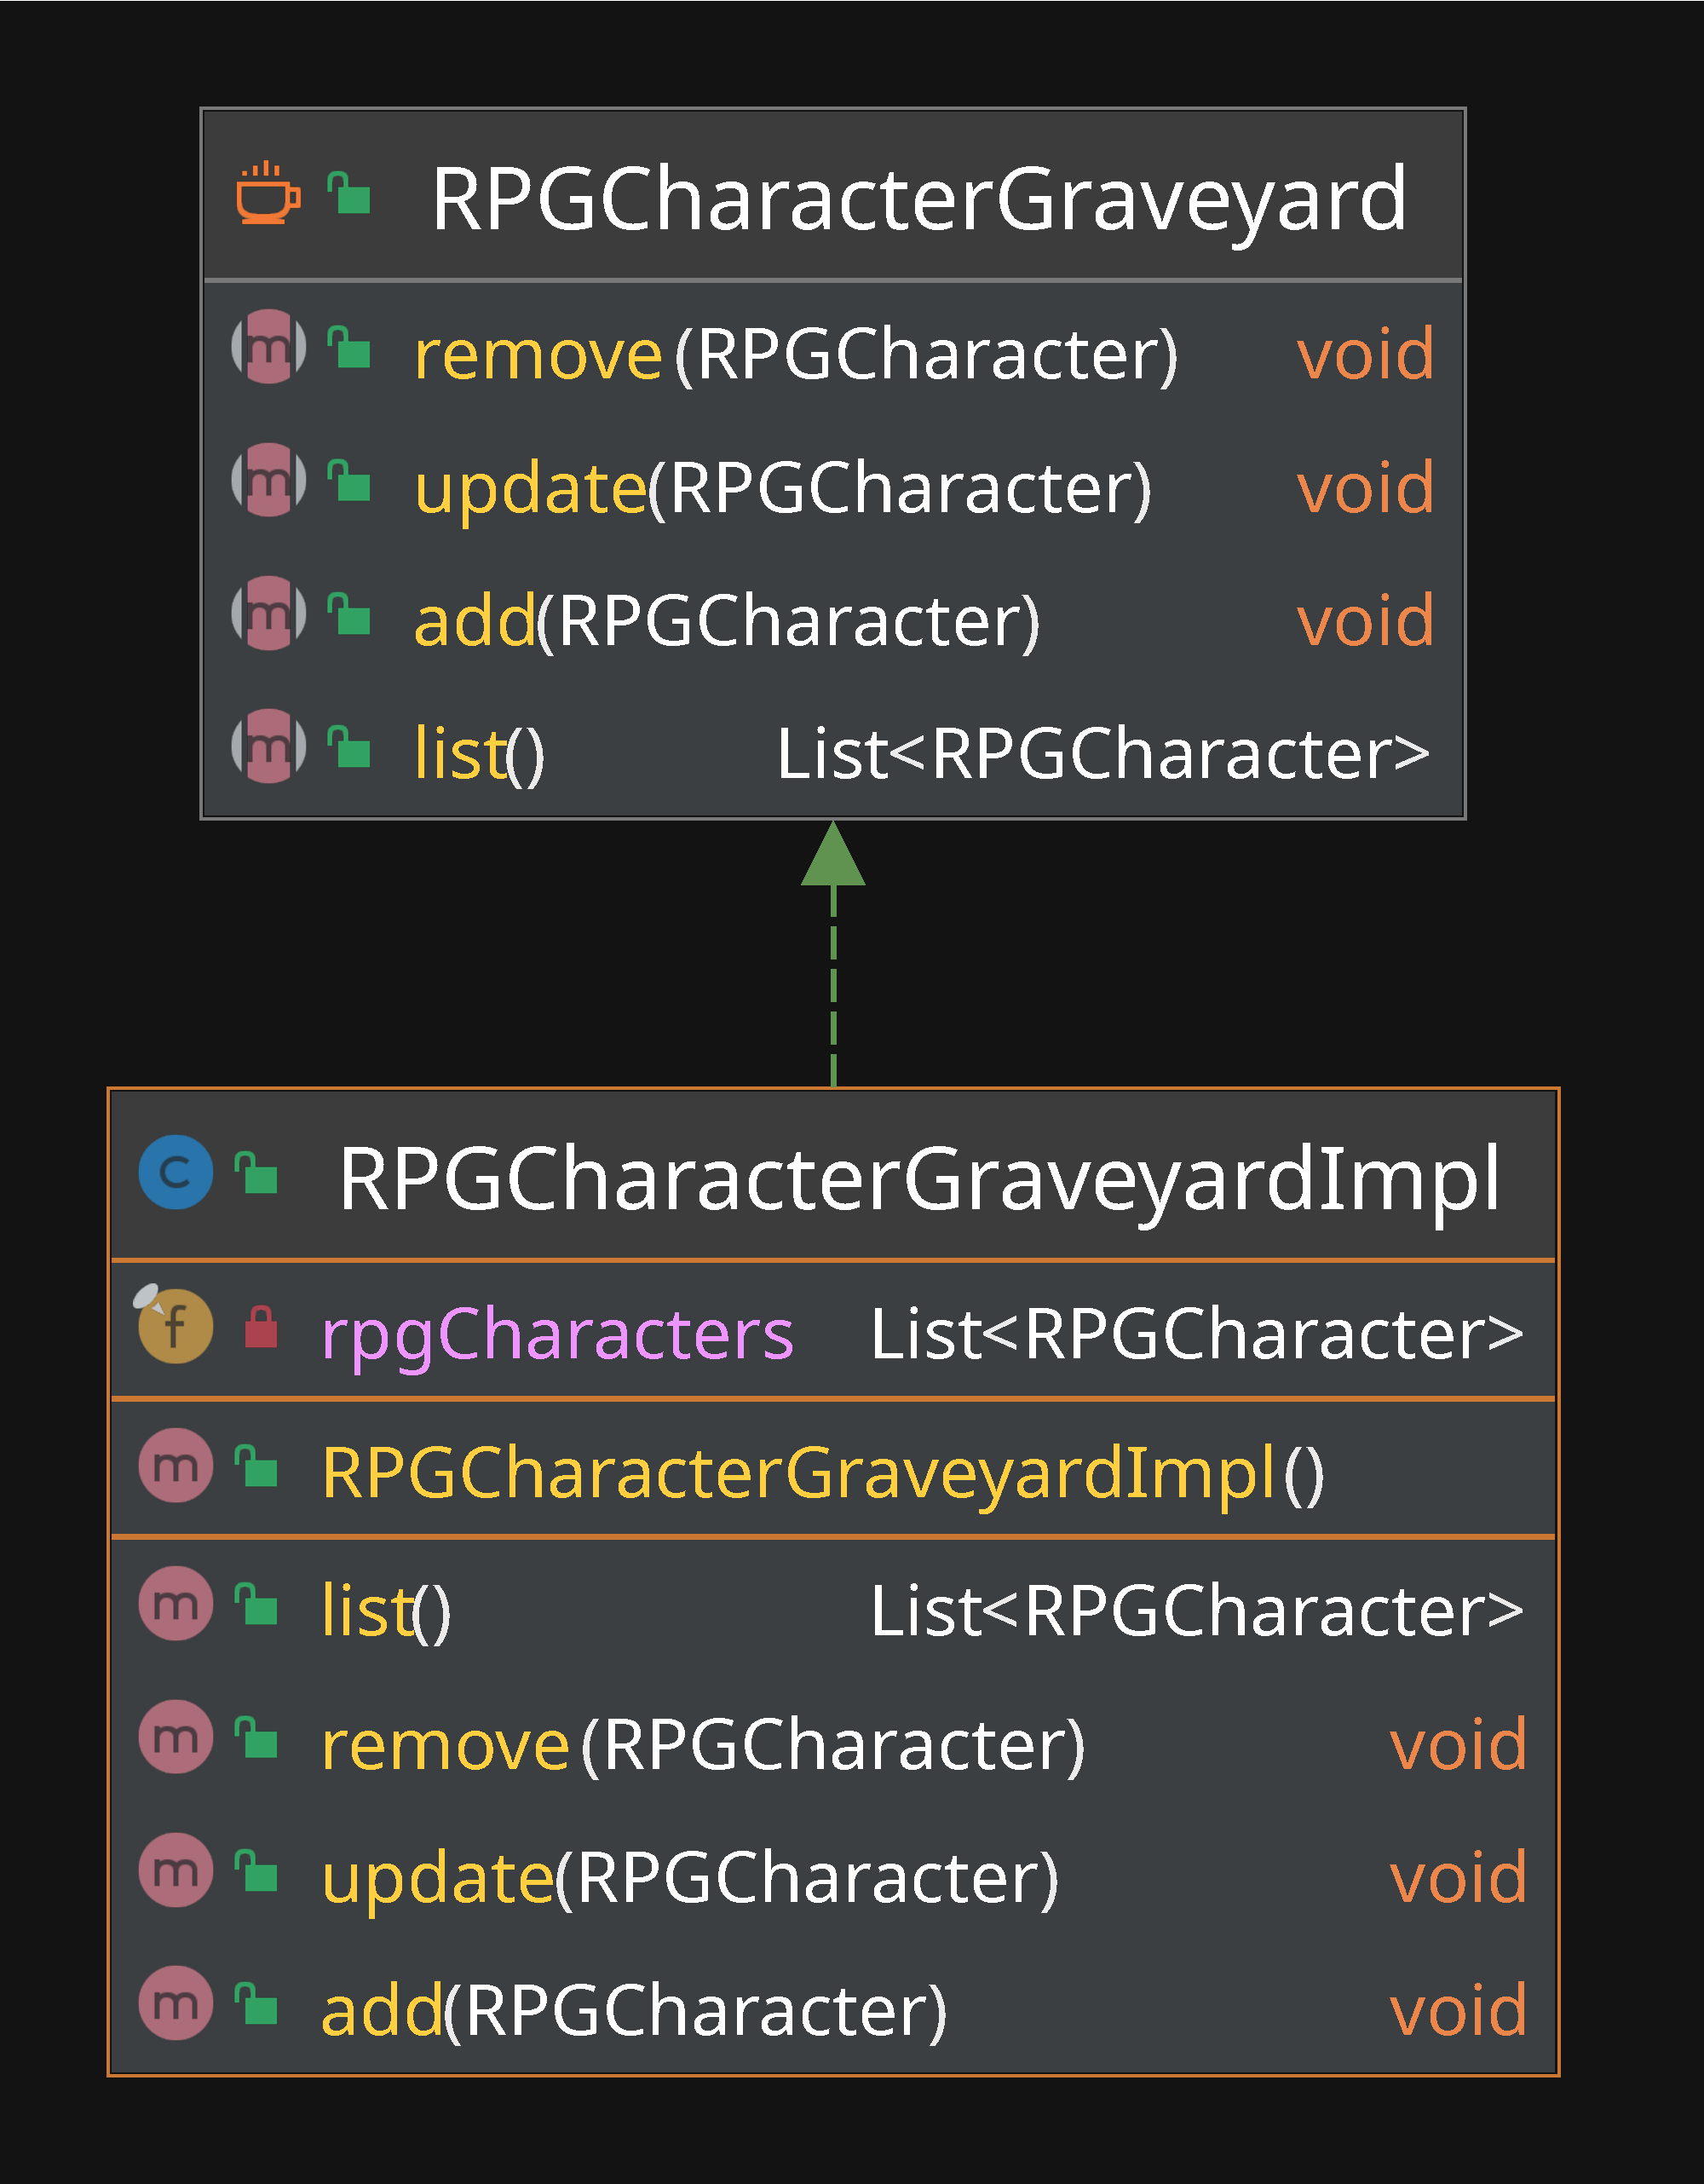
\includegraphics[width=0.4\textwidth]{Bilder/RPGCharacterGraveyardImpl.pdf}
	\caption{UML der RPGChracter und der RPGCharacterFactory Klasse}
	\label{fig:Stellvertreter}
\end{figure}
Zur Realisierung der Repositorys wurde das Entwurfsmuster des Stellvertreters verwendet. Abbildung \ref{fig:Stellvertreter} zeigt die UML Diagramme des \texttt{RPGCCharacterGraveyards} und deren Implementation. Da die Implementation der Repositorys Gerät bzw. Implementationsabhängig ist, wird in den unteren Schichten ausschließlich mit den Interfaces als Stellvertreter für die tatsächliche Implementation gearbeitet. In den äußeren Schichten kann so die tatsächliche Persistierung mittels des Interfaces implementiert werden, die unteren Schichten kennen allerdings nur das Interface und somit ausschließlich den Stellvertreter. Wie die Funktionalität genau realisiert wird ist in den unteren Schichten nicht von relevanz.


% ---- Literaturverzeichnis
%\cleardoublepage
%\renewcommand*{\chapterpagestyle}{plain}
%\pagestyle{plain}
%\pagenumbering{Roman}                   % Römische Seitenzahlen
%\setcounter{page}{\numexpr\value{savepage}+1}
%\printbibliography[title=Literaturverzeichnis]

% ---- Anhang
\appendix
%\clearpage
%\pagenumbering{Roman}  % römische Seitenzahlen für Anhang

\newpage
\end{document}
